%
%
\documentclass[12pt]{report}
% \includeonly{}
%
%			PREAMBOLO
%
\usepackage[a4paper]{geometry}
\usepackage{amssymb,amsmath,amsthm}
\usepackage{graphicx}
\usepackage{url}
\usepackage{hyperref}
\usepackage{epsfig}
\usepackage[italian]{babel}
\usepackage{tesi}
\usepackage{float} % per le immagini
\usepackage{enumitem} % per gli elenchi
\usepackage[T1]{fontenc}
\usepackage[utf8]{inputenc}
\usepackage{hyperref}
\usepackage{verbatim} %commenti
\usepackage{framed}
\usepackage{setspace}
%


\newtheorem{myteor}{Teorema}[section]
%
\newenvironment{teor}{\begin{myteor}\sl}{\end{myteor}}
%
%
%			TITOLO
%
\begin{document}
\begin{center}
	
\includegraphics[height=3.0cm]{logo_unimi.png}
\end{center}


\title {\textbf{Sviluppare il pensiero \\[1mm]computazionale con i quesiti Bebras: \\[1mm]approcci e strumenti per l'uso nella \\[1mm]pratica scolastica\\[1mm]}} 
\author{Annalisa CALCAGNI}
\dept{Corso di Laurea Magistrale in Informatica } 
\anno{2016-2017}
\matricola{865610}
\relatore{Prof. Violetta LONATI}
\correlatore{Prof. Mattia MONGA}
%
%			DEDICA
%

\beforepreface

%        {\hfill \Large {\sl a nonna Maria}}

% 
\afterpreface
\doublespacing
%			PREFAZIONE: Introduzione
%
\prefacesection{Introduzione}

\begin{comment} PER INTRODUZIONE
Il ``Bebras dell'Informatica'' è un concorso internazionale che offre agli studenti delle scuole primarie e secondarie la possibilità di avvicinarsi al mondo dell'informatica in modo divertente attraverso una gara non competitiva.
\end{comment}

Il lavoro descritto in questa tesi ha come obiettivo principale quello di analizzare la situazione attuale nella scuola primaria e secondaria di primo grado della didattica dell'informatica e proporre uno strumento per l'insegnamento di questa disciplina.
Infatti l'insegnamento dell'informatica riveste un ruolo importante per i seguenti motivi \cite{InformaticaScuola}:
\begin{itemize}
	\item \textit{incrementa la creatività} grazie ai numerosi metodi che offre per affrontare e risolvere un problema;
	\item \textit{sviluppa la costruttività} grazie alla progettazione di algoritmi;
	\item \textit{aiuta a padroneggiare la complessità}, infatti affrontare problemi informatici aiuta a risolvere questioni più complesse riguardanti altre aree;
	\item \textit{potenzia il ragionamento accurato} attraverso la scrittura di programmi in cui è necessaria l'esattezza in ogni minimo dettaglio.
\end{itemize}
Il ruolo dell'informatica, come quello della matematica, nella scuola primaria e secondaria è duplice: \textit{pratico} perché qualsiasi lavoro svolgeranno in futuro gli studenti la componente digitale sarà importante, e contemporaneamente \textit{formativo} perché l'informatica è un valido strumento intellettuale per sviluppare abilità concettuali essenziali qualunque sia lo sviluppo professionale degli alunni.


L'aspetto scientifico dell'informatica aiuta a sviluppare competenze logiche e capacità di risoluzione dei problemi cioè il pensiero computazionale: una risorsa per promuoverlo fin dai primi anni di scuola sono i quesiti Bebras. Questi sono problemi proposti nelle gare Bebras: un concorso internazionale organizzato annualmente per gli studenti delle scuole primarie e secondarie il cui scopo è la divulgazione scientifica dell'informatica.

In questo lavoro di tesi ci si concentra sulla situazione nella scuola italiana primaria e secondaria di primo grado, in cui l'informatica è insegnata come utilizzo del computer piuttosto che come disciplina scientifica.
\`{E} stata fatta un'analisi delle Indicazioni Nazionali per il curricolo del primo ciclo d'istruzione fornite dal Ministero dell'Istruzione e sono stati trovati dei collegamenti ``nascosti'' all'informatica.
Successivamente è stato fatto un lavoro di analisi e corrispondenza tra i quesiti della gara Bebras e le Indicazioni Nazionali per verificare come questi quesiti possano essere utilizzati all'interno del curricolo scolastico.
Dopo aver evidenziato i legami tra i quesiti Bebras e gli obiettivi didattici indicati dal Ministero dell'Istruzione, è nata l'esigenza di permettere ai docenti di reperire questo materiale. \`{E} stata quindi proposta una classificazione dei quesiti tramite la lente di lettura della definizione operazionale del pensiero computazionale che evidenzia gli aspetti educativi e le potenzialità didattiche di ogni quesito.
Infine è stata sviluppata un'applicazione web il cui scopo è rendere accessibili a tutti i docenti i quesiti Bebras proponendo per ognuno di essi la relativa soluzione, spiegazione e corrispondenze sia con le Indicazioni Nazionali che con lil pensiero computazionale.
\\

La tesi ha la struttura seguente. Il capitolo \ref{cap1} presenta le gare Bebras e i quesiti contenuti in questo concorso, quindi viene esposto un excursus sulle classificazioni dei quesiti proposte fino ad ora.
Il capitolo \ref{cap2} riporta la situazione attuale nella scuola italiana dell'insegnamento dell'Informatica nella primaria e secondaria di primo grado e viene evidenziata la corrispondenza tra le Indicazioni Nazionali proposte dal Ministero dell'Istruzione e i quesiti Bebras.
Il capitolo \ref{cap3} richiama il concetto di pensiero computazionale e la sua definizione operazionale che viene utilizzata come lente di lettura per una classificazione dei quesiti Bebras, quindi riporta le osservazioni ottenute dalle interviste fatte ai docenti sull'uso e la comprensione della suddetta classificazione.
Infine l'appendice presenta l'applicazione web sviluppata per rendere usufruibile ai docenti i quesiti Bebras.
%
%
% 
% 
%			CAPITOLO 1: Bebras
\chapter{I giochi Bebras dell'Informatica}
\label{cap1}
% nell'introduzione si definisce cos'è il bebras
I giochi Bebras dell'Informatica nascono in Lituania da un'idea di Valentina Dagiene, docente presso l'Università di Vilnius, che vuole trovare uno strumento divertente per avvicinare i ragazzi alla disciplina informatica. Per fare ciò Dagiene sceglie di organizzare dei giochi sotto la forma di gara: la competizione infatti risulta essere un metodo didattico vincente per attirare l'attenzione degli studenti e suscitare il loro interesse. Nel panorama internazionale, da prima della nascita del Bebras dell'informatica, sono già presenti gare informatiche: una delle più famose sono le ``Olimpiadi internazionali dell'informatica'' il cui scopo è selezionare studenti particolarmente talentuosi in questa disciplina. Le gare Bebras, invece, pongono l'attenzione sulla divulgazione dell'informatica come disciplina scientifica, si tratta infatti di una gara non competitiva.

Il nome ``Bebras'', in lituano \textit{castoro}, é stato scelto perché le caratteristiche dell'animale stesso quali la laboriosità, la creatività, la tenacità e la vivacità siano stimolate nei partecipanti a queste gare.

La prima edizione dei giochi Bebras si svolge nel 2004 solo in Lituania ma pochi anni dopo queste gare diventano una realtà internazionale: nel 2006 vengono organizzate anche in Estonia, Germania, Olanda e Polonia e nel 2016 sono 50 i Paesi coinvolti.
Per ogni Paese partecipante alle gare Bebras esiste un gruppo locale che si occupa di tutto ciò che riguarda l'organizzazione della competizione nella propria nazione, come la scelta e la traduzione dei quesiti e la gestione della tecnologia utilizzata per lo svolgimento delle gare.

Le gare Bebras si svolgono ogni anno indicativamente nella stessa settimana di novembre in tutti i Paesi partecipanti, esclusi quelli dell'emisfero sud. 
Questa gare sono rivolte a studenti di varie età: ogni Paese decide come suddividere in categorie i propri partecipanti in base all'età e quali quesiti associare ad ogni categoria.

In Italia i partecipanti alle gare Bebras sono divisi in categorie in relazione alla classe frequentata:
\begin{itemize}
	\item \textbf{KiloBebras}: alunni delle Scuole Primarie [8-10 anni circa]
	\item \textbf{MegaBebras}: alunni delle classi prima e seconda delle Scuole Secondarie di primo grado [10-12 anni circa]
	\item \textbf{GigaBebras}: alunni delle classi terze delle Scuole Secondarie di primo grado [12-13 anni circa]
	\item \textbf{TeraBebras}: alunni del biennio delle Scuole Secondarie di secondo grado [13-15 anni circa]
	\item \textbf{PetaBebras}: alunni del triennio delle Scuole Secondarie di secondo grado [15-18 anni circa]
\end{itemize}
Nell'edizione italiana dei giochi Bebras si partecipa a squadre: lo scopo è di enfatizzare l'importanza del lavoro di gruppo che è fondamentale nella disciplina informatica. 

Lo svolgimento delle gare avviene attraverso la registrazione via web di un insegnante referente che si occupa di iscrivere le squadre e di sorvegliare lo svolgimento nel proprio Istituto. Il giorno della gara ciascuna squadra, formata da 4 studenti, si collega usando un computer alla piattaforma Bebras \cite{PiattaformaBebras} tramite un browser.  
Nelle settimane successive alla gara le squadre partecipanti possono vedere sul sito Bebras tutti i quesiti svolti con l'indicazione dei punteggi ottenuti e delle risposte corrette con le relative spiegazioni. \`{E} auspicabile che i docenti delle classi partecipanti ai giochi Bebras discutano con gli studenti le correzioni dei quesiti, creando così un'occasione per approfondire o chiarire gli argomenti trattati.

L'organizzazione italiana Bebras pone grande attenzione sulla scelta e formulazione dei quesiti da proporre nella gara perché, come si vedrà nel successivo capitolo, questi possono essere uno strumento didattico da utilizzare anche al di fuori del contesto competitivo.
\bigskip

Una questione molto sentita all'interno della comunità, già dalle prime edizioni delle gare, è quali tematiche informatiche trattare e quindi come presentare l'informatica.
Infatti non esistono dei sillabi universalmente riconosciuti per questa disciplina, non vi è quindi una linea comune su ciò che dovrebbe essere incluso in una competizione informatica.
Nelle prime edizioni delle gare la comunità Bebras prende spunto dalle raccomandazioni dell'UNESCO (Organizzazione delle Nazioni Unite per l'Educazione, la Scienza e la Cultura) e dal sillabo dell'ECDL (patente europea per l'uso del computer). Nelle prime gare infatti oltre a problemi riguardanti il pensiero algoritmico, la programmazione e altri temi tipicamente informatici sono presenti numerosi problemi sull'uso di sistemi informatici e su aspetti sociali ed etici.
Questi temi trattati all'interno delle gare rispecchiano pienamente il titolo dei giochi Bebras fino al 2015: ``\textit{Bebras International Contest on Informatics and Computer Literacy}'' dove per \textit{Computer Literacy} si intende l'alfabetizzazione digitale e quindi l'uso degli strumenti informatici.
Gradualmente la scelta dei temi da trattare subisce importanti modifiche e di anno in anno nella gara diminuiscono sempre più i problemi legati all'applicazione dell'informatica mentre sono sempre più numerosi i problemi riguardanti gli aspetti scientifici di tale disciplina. All'interno della comunità Bebras si fa sempre più chiara la volontà di presentare l'informatica come scienza e non come uso di applicazioni. Nel 2015 il titolo delle gare diventa ``Bebras International Challenge on Informatics and Computational Thinking'': questo cambio denota ufficialmente che non sono più proposti problemi sulla digitalizzazione bensì si pone l'attenzione sullo sviluppo del pensiero computazionale.

Le gare Bebras sono composte da un insieme di quesiti: giochi e rompicapi ispirati a reali problemi di natura informatica. I quesiti possono essere affrontati senza alcuna conoscenza specifica e diventare lo stimolo per successivi approfondimenti.
Annualmente è organizzato un workshop internazionale in cui si riuniscono i delegati dei Paesi partecipanti, con lo scopo di proporre e correggere i quesiti di cui è composta la gara. 
Ogni Paese partecipante è invitato a fornire almeno un mese prima del workshop un insieme di proposte di quesiti, che sono disponibili all'interno della comunità per essere visionati e commentati. Durante i tre giorni del workshop i partecipanti vengono divisi in gruppi, ad ognuno dei quali viene assegnato un insieme di quesiti su cui lavorare. Al termine del lavoro ogni gruppo proporrà una serie di quesiti candidati ad essere quelli maggiormente consigliati ma diverranno tali solo dopo la votazione finale di ogni partecipante.
A conclusione del workshop quindi si ottiene un insieme consistente di quesiti dal quale verranno scelti quelli da proporre nelle gare locali.

%
%
\section{I quesiti Bebras}

I quesiti Bebras, come detto nella sezione precedente, sono i problemi che compongono una gara.
Di seguito si riportano alcuni esempi dell'edizione italiana delle gare; si può notare che non vengono richieste conoscenze pregresse, ma lo scopo è che gli studenti scoprano i concetti informatici attraverso divertenti problemi.

\begin{figure}[H]
	\centering
	\fbox{\includegraphics[height=10.0cm]{"./immagini/01_Cap1/2016-HU-02Testo"}}
	\caption{ ``\textit{La ricetta segreta}'' quesito Bebras dell'edizione italiana del 2016 proposto ai partecipanti tra 8-10 anni}\label{fig:ricetta}
\end{figure}

Il quesito ``La ricetta segreta'' (Figura \ref{fig:ricetta}) è stato proposto nella gara italiana svolta nel 2016 da studenti tra gli otto e i dieci anni.
La lista degli ingredienti è un esempio della struttura dati chiamata lista. Il foglio che indica l'ingrediente successivo costituisce il puntatore all'elemento successivo della lista. Per accedere alla lista occorre avere il puntatore al primo elemento della lista.

\begin{figure}[H]
	\centering
	\fbox{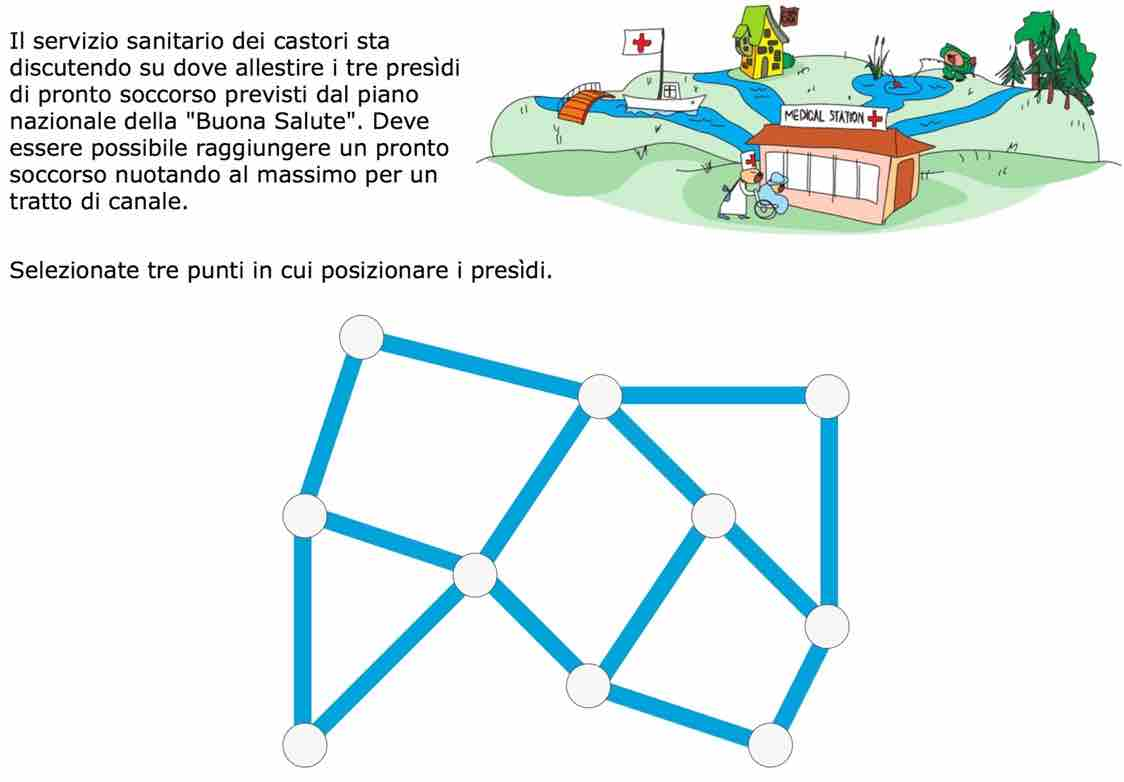
\includegraphics[height=10.0cm]{./immagini/01_Cap1/2016-CH-03Testo}}
	\caption{``\textit{Pronto soccorso}'' quesito Bebras dell'edizione italiana 2016 proposto ai partecipanti tra 10-15 anni}\label{fig:prontosoccorso}
\end{figure}

Il quesito ``Pronto soccorso'' (Figura \ref{fig:prontosoccorso}) è stato incluso nell'edizione italiana della gara svolta nel novembre 2016 da studenti tra i dieci e i quindici anni.
La rete di canali raffigurata può essere rappresentata da un grafo, in cui i tratti di canale sono gli archi (non orientati, cioè percorribili in entrambi i sensi) e i punti dove essi si incontrano sono i nodi. Il quesito proposto è un esempio del problema dell'insieme dominante nella versione in cui si tratta di decidere se un insieme dominante esiste. 

I quesiti sono interessanti, accattivanti e fanno riferimento a situazioni reali per attirare l'attenzione dei partecipanti. La comunità Bebras lavora sui quesiti in modo da renderli il più comprensibile possibile, per questo motivo spesso il testo è arricchito con figure esplicative, così che lo studente si concentri su come affrontare il problema piuttosto che sulla comprensione della richiesta. Inoltre la comunità pone una particolare attenzione sulla lunghezza dei quesiti: questi devono essere abbastanza corti da essere visibili per intero su un'unica schermata del computer. Ogni quesito ha il compito di avvicinare il partecipante all'apprendimento di un concetto informatico a cui spesso non si fa riferimento in maniera esplicita, inoltre il tema trattato è indipendente dal curriculum scolastico, che è differente per ogni Paese.

I quesiti comprendono la scelta tra risposte multiple, lo spostamento di blocchi o oggetti, la selezione di uno o più oggetti, associazioni che si realizzano cliccando sulla casella di partenza e poi su quella di arrivo o risposte aperte dove il partecipante deve inserire delle righe di codice.
Inoltre sono presenti anche quesiti interattivi in cui lo studente ha un feedback immediato della sua azione: ad esempio la selezione dei passi da far effettuare ad un robot che si muove in risposta agli input del partecipante.


Un aspetto molto importante e discusso dalle prime edizioni delle gare è la qualità dei quesiti: nel 2008 Dagiene e Futschek \cite{DagieneISEEP2008} individuano un elenco di requisiti che dovrebbe soddisfare un ``buon quesito''. Molte caratteristiche citate in questo elenco sono diventate standard e sono state ufficializzate nello statuto della comunità. Alcune criticità riguardanti l'elenco proposto sono evidenziate da Pohl e Hein \cite{PohlQuality}  nel 2015: gli autori osservano che non è possibile imporre un vincolo temporale di 3 minuti per la risoluzione di ogni quesito, infatti i quesiti più difficili potrebbero richiedere maggior tempo rispetto a quelli più facili e viceversa; per quanto riguarda il divieto di usare foglio e matita come aiuto allo svolgimento del problema, Pohl \textit{et al.} affermano invece che questo è un metodo importante nella disciplina informatica per ragionare e affrontare un problema complicato; infine sul vincolo della lunghezza di un quesito obiettano che non è possibile misurarla facendo riferimento alla grandezza dello schermo di un computer in quanto è un parametro variabile in base all'hardware utilizzato.

Un altro aspetto fondamentale molto sentito all'interno della comunità Bebras è l'assegnazione della corretta difficoltà ai quesiti. Il rischio infatti è di lasciare ai partecipanti la percezione che la gara risulti essere o troppo semplice o troppo difficile e quindi poco accattivante.
L'unico modo per stimare il livello di difficoltà di un quesito è quello di basarsi sull'esperienza e sull'intuito degli organizzatori: non vi è infatti una tecnica scientifica da poter applicare se non l'analisi delle gare svolte nei precedenti anni e i relativi risultati. A tal riguardo nel 2015 Bellettini \textit{et al.} \cite{BellettiniITICSE2015} analizzano i risultati dell'edizione italiana del 2014 delle gare Bebras attraverso un modello statistico per verificare se la difficoltà percepita dagli studenti è sostanzialmente diversa da quella stimata dagli organizzatori ottenendo come risultato che solo in un terzo dei casi i quesiti sono mal stimati. Oltre alle analisi delle gare a posteriori, nel 2013 Wilem van der Vegt \cite{WilemDifficulty} stila un questionario da proporre agli organizzatori, prima dell'assegnazione del livello di difficoltà dei quesiti, per far emergere eventuali elementi che possano essere cause di difficoltà per i partecipanti alle gare.

Un ulteriore tema affrontato nella comunità Bebras è relativo alla classificazione dei quesiti che verrà approfondito nella Sezione 2.

%
%
%	
\section{Classificazione dei quesiti Bebras}\label{Classificazione}
Durante il workshop annuale, come visto nella sezione precedente, viene creato un insieme di quesiti Bebras dal quale le delegazioni locali selezionano quelli da proporre nella gara del proprio Paese. Quindi all'interno della comunità nasce l'esigenza di associare i quesiti a categorie riguardanti temi informatici così da facilitare la selezione locale dei quesiti e poter presentare questa disciplina nel modo più completo possibile.

Una prima proposta di classificazione è stata messa a punto nel 2008 da Dagiene e Futschek \cite{DagieneISEEP2008}, ed è stata utilizzata come riferimento per la preparazione delle gare fino al 2016, una seconda nel 2009 da Kalas e Tomcsanyiova [12]. Si tratta in entrambi i casi di elenchi di argomenti informatici proposti e non di vere e proprie classificazioni. Inoltre gli articoli non illustrano come associare quesiti e categorie, né forniscono esempi a riguardo.
L'elenco di argomenti informatici proposto è il seguente:

\begin{enumerate}
	\item \textbf{concetto informatico di informazione} (INF): rappresentazione (simbolica, numerica, visiva), codifica e crittografia
	
	\item \textbf{pensiero algoritmico} (ALG) inclusi gli aspetti relativi alla programmazione
	
	\item \textbf{uso di sistemi informatici} (USE) ad esempio l'utilizzo di motori di ricerca, e-mail, fogli di calcolo con un accento sui principi generali senza riferimento ad uno specifico sistema
	
	\item \textbf{strutture, pattern e disposizioni} (STRUCT) con riferimento a problemi di calcolo combinatorio e strutture dati come i grafi
	
	\item \textbf{puzzle} (PUZ): puzzle e giochi logici
	
	\item \textbf{impatto dell'informatica sulla società} (SOC) dal punto di vista etico, culturale, legale e sociale
\end{enumerate}

Nel 2009 Kalas e Tomcsanyiova \cite{KalasIFIP2009} propongono una rivisitazione delle categorie proposte in \cite{DagieneISEEP2008}: l'uso dei sistemi informatici e l'impatto sulla società (3 e 6) vengono accorpati in ``Alfabetizzazione digitale''; gli argomenti riguardanti l'informazione e le strutture (1 e 4) sono unificate sotto il titolo ``Gestione dei dati''; in ``Problem solving''  è incluso l'ambito dei puzzle (5) insieme al ragionamento logico, la giustificazione, l'argomentazione, le strategie per la risoluzione dei problemi; infine all'interno di ``Programmazione'' vengono inseriti il tema del pensiero algoritmico (2), la descrizione formale di una soluzione, di un processo, di un comportamento, la comprensione, l'analisi, l'interpretazione e la composizione di tali descrizioni. 
 
Entrambe le proposte contengono categorie riguardanti l'utilizzo del computer e questioni sociali: le gare Bebras, come detto nella sezione precedente, nei primi anni presentano alcuni quesiti focalizzati sull'alfabetizzazione digitale. Negli anni successivi i quesiti di questa tipologia si riducono sempre di più fino a scomparire e gradualmente l'obiettivo delle gare Bebras diventa quello di presentare l'informatica intesa come disciplina scientifica e di sviluppare il pensiero computazionale. 
Il cambio di obiettivo fa sentire la necessità di nuove classificazioni in cui si prendano in considerazione i cambiamenti avvenuti. A tal riguardo sono state proposte la classificazione di Pohl e Westmeyer \cite{PohlLNCS2015} nel 2015, basata esclusivamente su argomenti informatici, e quella di Dagiene \textit{et al.} \cite{DagieneINFORMATICA2017} in cui sono considerate sia le aree informatiche che il pensiero computazionale.

Pohl e Westmeyer \cite{PohlLNCS2015} vogliono ottenere una struttura che permetta una classificazione a grana fine, che sia organizzata gerarchicamente per permettere la categorizzazione su diversi livelli di dettaglio ed infine che permetta la categorizzazione su concetti sia generali che specifici.
Essi considerano tre possibili modi per caratterizzare aspetti e concetti essenziali dell'informatica: il vocabolario del pensiero computazionale, le aree definite nell'istruzione scolastica tedesca e le \textit{idee fondamentali dell'informatica} esposte da Schwill \cite{SchwillEATCS1994}.

Queste ultime sono le aree informatiche individuate da Andreas Schwill nel 1994 \cite{SchwillEATCS1994}: egli vuole indicare e formalizzare, ai fini dell'insegnamento, i concetti alla base dell'informatica che non variano con l'evoluzione delle tecnologie.
Schwill analizza le fasi dello sviluppo software e raggruppa gli argomenti emersi dall'analisi in tre strutture gerarchiche, le cui radici sono: l'algoritmizzazione, che si espande in concetti di programmazione, valutazione della complessità, verifica della correttezza, processi concorrenti; l'organizzazione strutturale, i cui nodi figli sono la modularizzazione e gerarchizzazione; infine il linguaggio, che comprende sintassi e semantica.


Pohl e Westmeyer sostengono che tra i modi ipotizzati per la classificazione solo utilizzando la gerarchia presentata da Schwill si possa ottenere una struttura gerarchica.
Essi propongono quindi una classificazione composta da quattro alberi: quelli con radice ``Formalizzazione'' (Figura 4), ``Algoritmizzazione'' (Figura 5) e ``Organizzazione strutturale'' (Figura 6) sono una rielaborazione delle tre \textit{idee di Schwill}, mentre il quarto albero è ideato dagli autori stessi (Figura 3) e la sua radice è denominata ``Informazione''.

\begin{figure}[H]
	\centering
	\fbox{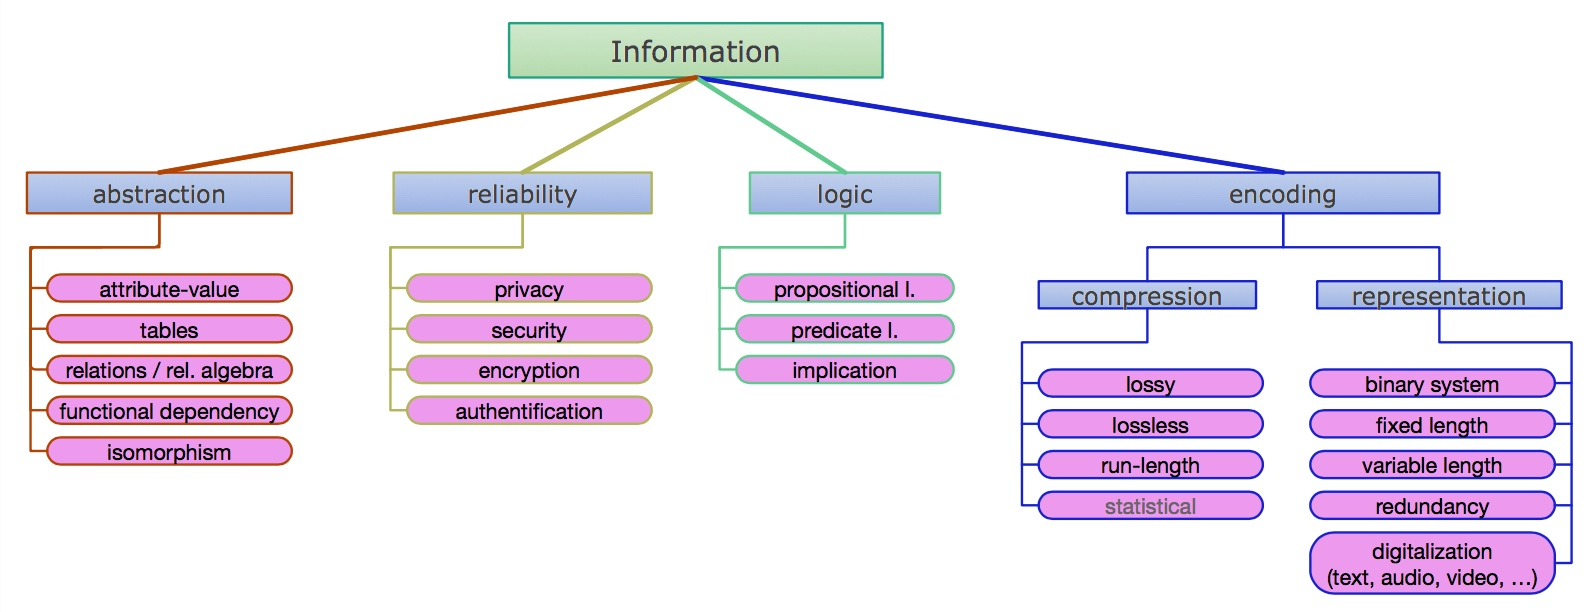
\includegraphics[width=15.0cm]{./immagini/01_Cap1/ClassificazionePohl_01}} \label{Informazione}
	\caption{Albero relativo a ``Informazione'' \cite{PohlLNCS2015}}
\end{figure}

\begin{figure}[H]
	\centering
	\fbox{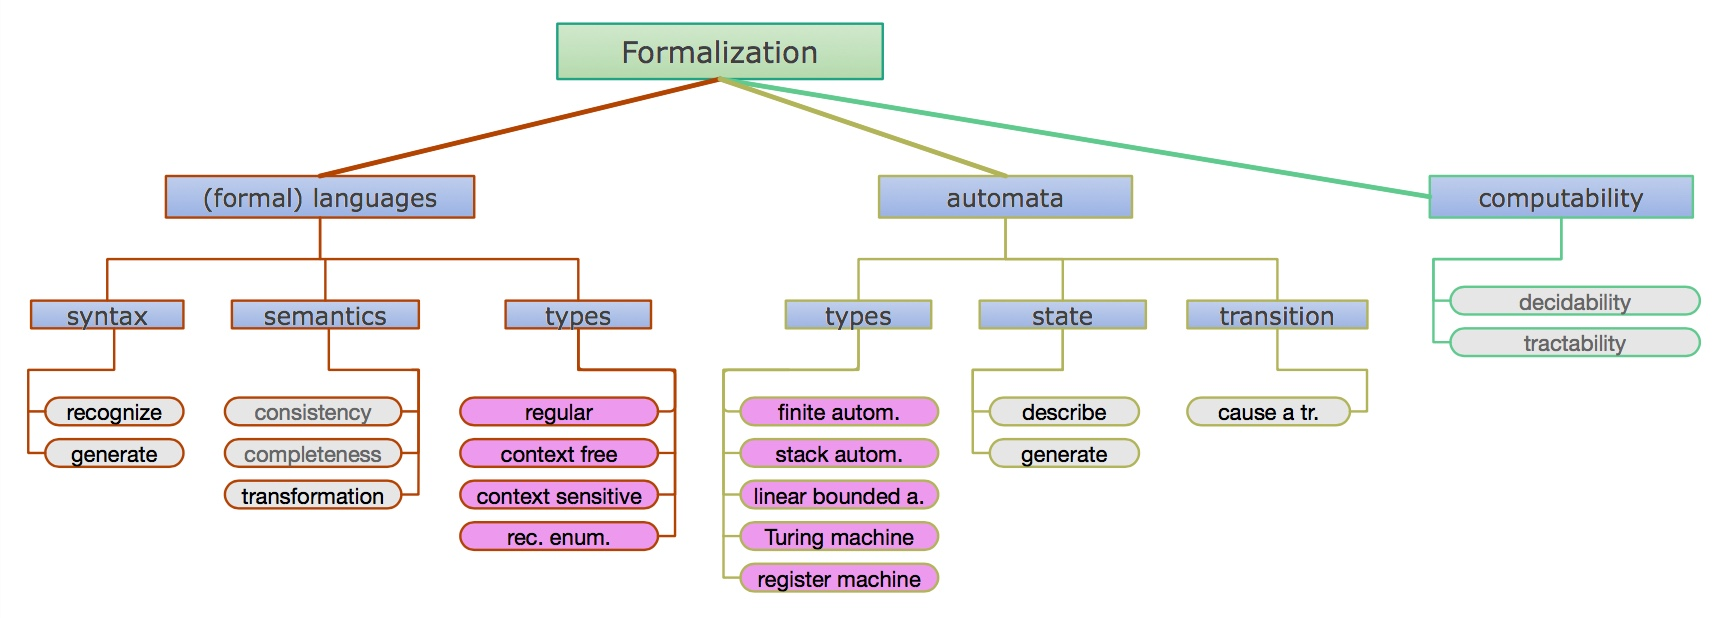
\includegraphics[width=15.0cm]{./immagini/01_Cap1/ClassificazionePohl_02}} \label{Formalizzazione}
	\caption{Albero relativo a ``Formalizzazione'' \cite{PohlLNCS2015}}
\end{figure}

\begin{figure}[H]
	\centering
	\fbox{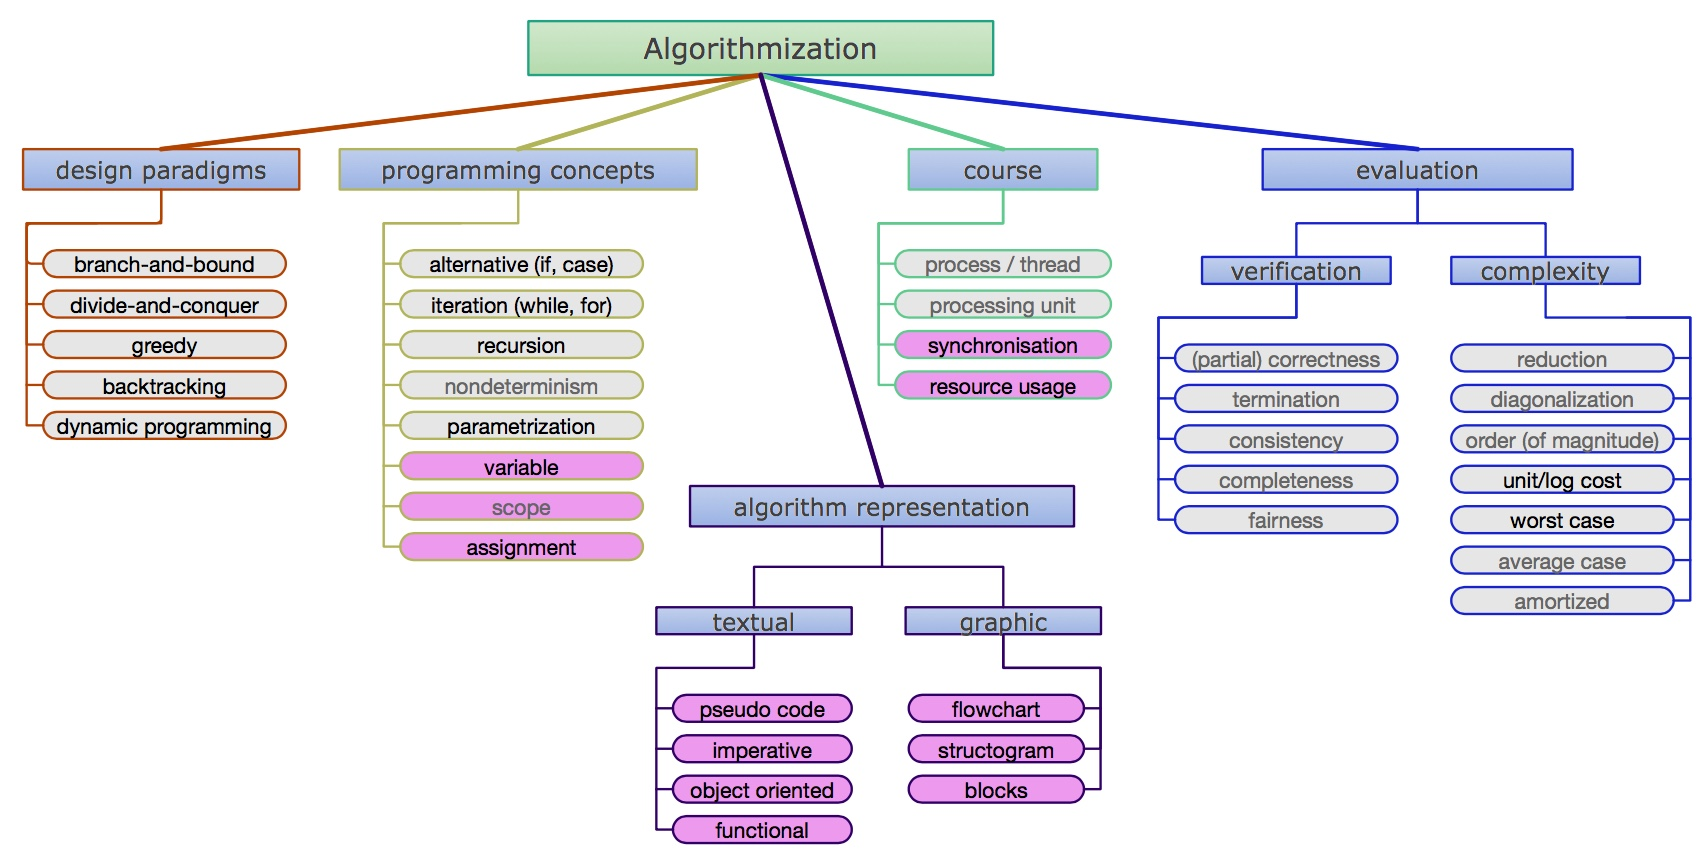
\includegraphics[width=15.0cm]{./immagini/01_Cap1/ClassificazionePohl_03}} \label{Algoritmizzazione}
	\caption{Albero relativo a ``Algoritmizzazione'' \cite{PohlLNCS2015}}
\end{figure}

\begin{figure}[H]
	\centering
	\fbox{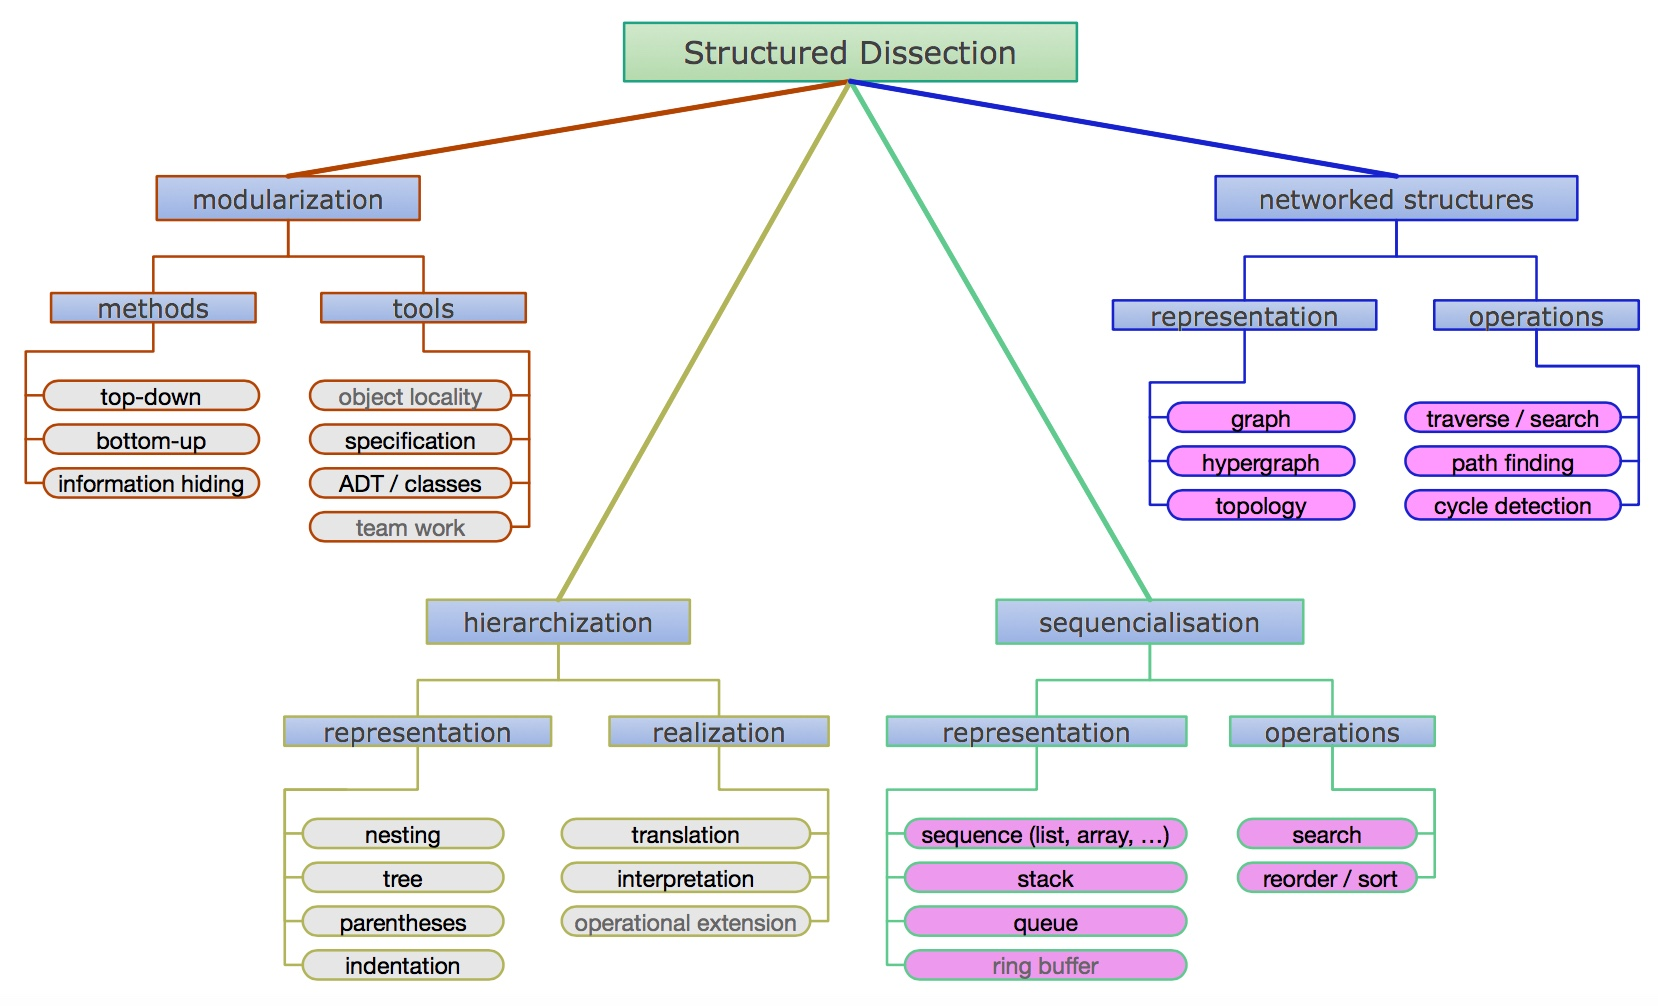
\includegraphics[width=15.0cm]{./immagini/01_Cap1/ClassificazionePohl_04}} \label{Organizzazione strutturale}
	\caption{Albero relativo a ``Organizzazione strutturale'' \cite{PohlLNCS2015}}
\end{figure}



La proposta di Pohl \textit{et al.} \cite{PohlLNCS2015} è stata pubblicata come poster, quindi senza esempi o spiegazioni su come applicare questa classificazione sui quesiti Bebras.

All'interno del contesto di cambiamento di obiettivo delle gare Bebras, nel 2017 Dagiene, Sentance e Stupuriene \cite{DagieneINFORMATICA2017} propongono una nuova classificazione bidimensionale basata su due aspetti: gli argomenti informatici indicati nei riferimenti curricolari per le scuole e le abilità del pensiero computazionale.
Questa proposta è mirata non solo all'utilizzo all'interno della comunità Bebras come sistema di riferimento per la classificazione dei quesiti, bensì anche per permettere ai docenti di cercare e scegliere i quesiti che possono essere utili ad attività didattiche da proporre in classe.


Gli argomenti informatici sono suddivisi in cinque aree:
\begin{enumerate}
	\item Algoritmi e programmazione
	\item Dati, strutture dati e rappresentazioni
	\item Processi informatici e hardware
	\item Comunicazioni e reti
	\item Interazione uomo-computer, sistemi e società
\end{enumerate}

Dagiene \textit{et al.}, per facilitare l'assegnazione dei quesiti a queste aree informatiche, forniscono un elenco di parole chiave (Figura \ref{parole-chiave}) che descrive ogni categoria.
 
Questa dimensione è stata adottata come riferimento per le gare Bebras del 2017.

\begin{figure}[H]
	\centering
	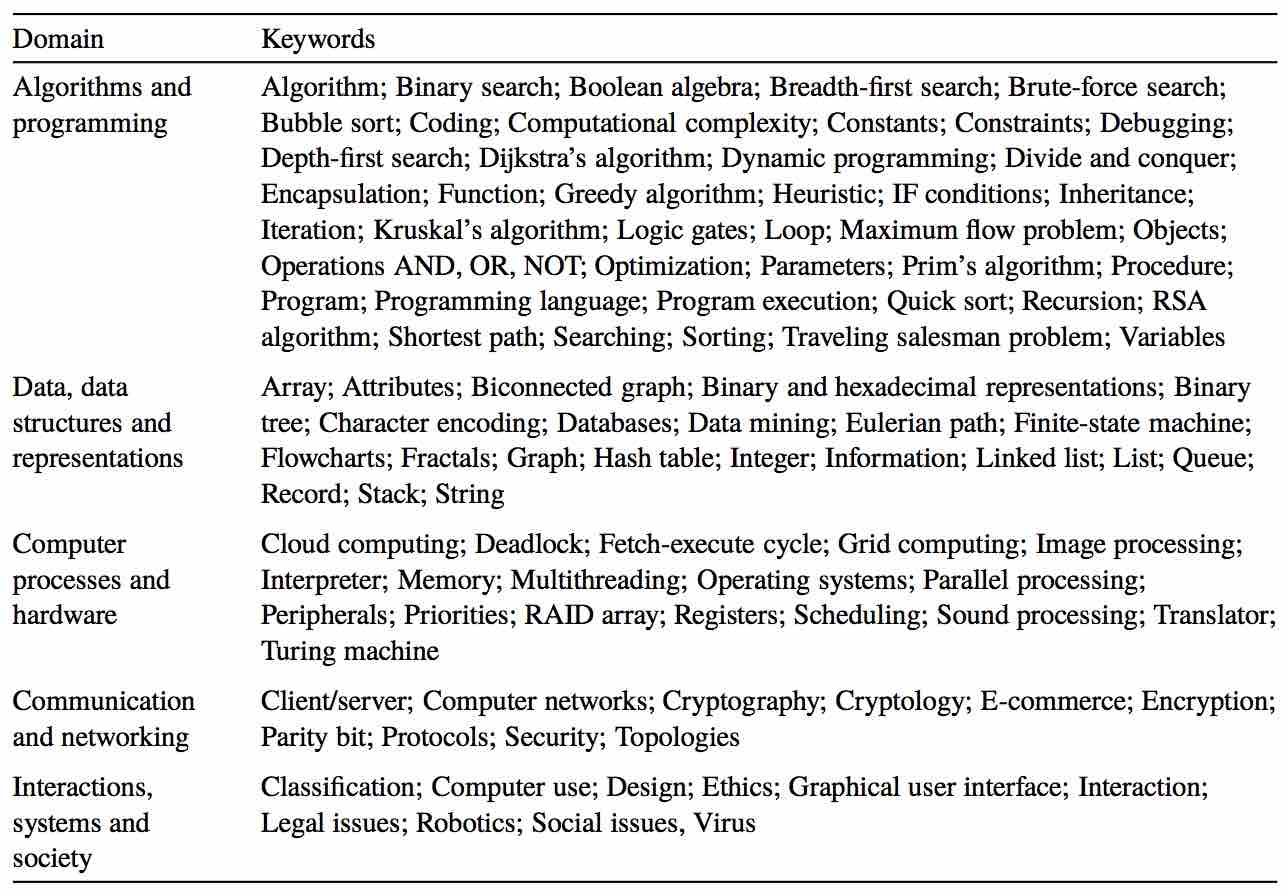
\includegraphics[height=11.3cm]{./immagini/01_Cap1/informaticContentDagiene}
	\caption{Parole chiave per ogni area informatica \cite{DagieneINFORMATICA2017}}\label{parole-chiave}
\end{figure}

La seconda dimensione riguarda le abilità del pensiero computazionale, in particolare la categorizzazione adottata nelle scuole inglesi, che è composta dalle seguenti aree:
\begin{enumerate}
	\item Astrazione;
	\item Pensiero algoritmico;
	\item Scomposizione;
	\item Valutazione;
	\item Generalizzazione.
\end{enumerate}

Per ogni area viene fornito un elenco di operazioni (Figura \ref{CTDagiene}).
Un quesito può appartenere contemporaneamente a più di un'area di questa dimensione, infatti per raggiungere la soluzione di un quesito Bebras si possono intraprendere diverse strategie risolutive, e quindi sviluppare differenti abilità. 
Gli autori suggeriscono comunque un limite massimo di tre aree da associare ad ogni quesito.

\begin{figure}[H]
	\centering
	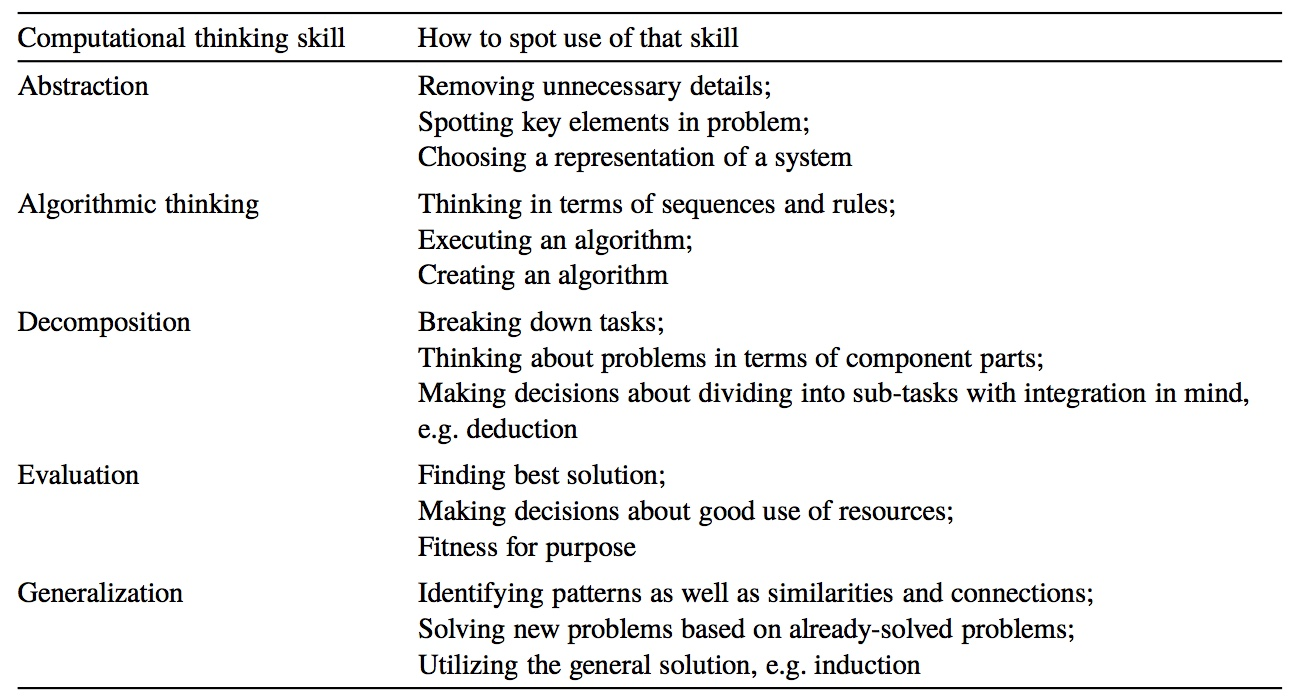
\includegraphics[height=9cm]{./immagini/01_Cap1/CTDagiene}
	\caption{Abilità del pensiero computazionale \cite{DagieneINFORMATICA2017}}\label{CTDagiene}
\end{figure}

A partire da queste due dimensioni si ottiene una matrice bidimensionale, in cui ogni quesito può essere posto in una sola categoria di concetti informatici ma in più categorie rappresentanti le abilità del pensiero computazionale (Figura \ref{TwoDimension}).
\begin{figure}[H]
	\centering
	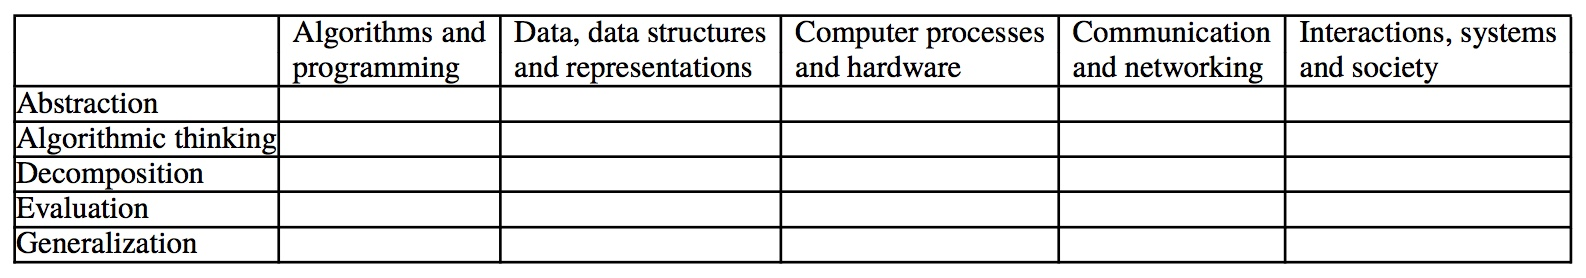
\includegraphics[height=2.7cm]{./immagini/01_Cap1/two-dimensional_classification}
	\caption{Classificazione a due dimensioni \cite{DagieneINFORMATICA2017}}\label{TwoDimension}
\end{figure}

Per quanto riguarda la dimensione degli argomenti informatici, si può osservare che la classificazione contiene un'area ``Interazione uomo-computer, sistemi e società'', con temi come uso del computer, design, e-commerce, aspetti legali e sociali, argomenti che di fatto non vengono più trattati nei quesiti Bebras. Per quanto riguarda l'effettiva applicazione della classificazione ai quesiti Bebras secondo le due dimensioni, nell'articolo non sono riportati esempi che la illustrino.

Un'altra prospettiva per classificare i quesiti Bebras è far emergere le abilità che vengono promosse in un dato quesito: in tale contesto si inserisce la proposta di Dagiene e Stupuriene del 2015 \cite{DagieneKEYCIT2015} basata sulla tassonomia di Bloom revisionata da Anderson \cite{Anderson}.

La tassonomia di Bloom è un metodo per classificare gli obiettivi di apprendimento in livelli di complessità negli ambiti cognitivo, affettivo e sensoriale. 
Il lavoro di Bloom e del suo team \cite{Bloom}, pubblicato nel 1956, è stato quello di raccogliere e analizzare migliaia di giudizi formulati da operatori scolastici e commissioni esaminatrici.
A partire dal materiale raccolto gli autori hanno cercato di derivare le categorie più frequentemente utilizzate nella valutazione e le hanno ordinate secondo un sistema gerarchico costituito da livelli disposti in ordine crescente di complessità: conoscenza, comprensione, applicazione, analisi, sintesi, valutazione.
La tassonomia di Bloom spesso è rappresentata da una piramide la cui base è l'attività più semplice da compiere e il vertice la più complessa.


Nel 2001 Anderson \textit{et al.} \cite{Anderson} propongono una versione rivista della tassonomia di Bloom per adeguarla alle mutate esigenze di docenti e studenti del XXI secolo.
Le modifiche apportate alla tassonomia originale sono le seguenti: i verbi sostituiscono i sostantivi utilizzati nella versione originale, la \textit{conoscenza} è sostituita con la \textit{memorizzazione}, la \textit{valutazione} dalla sommità della piramide passa al secondo posto ed infine alla \textit{sintesi} viene sostituita la \textit{creazione} che è posta al primo posto.
Anche questa versione rivisitata è rappresentata attraverso una piramide (Figura 10) e il metodo per interpretarla è lo stesso dell'originale: comprendere un concetto è più difficile di ricordarlo, analizzare un oggetto è più difficile di comprenderlo, creare qualcosa è più difficile di analizzarlo.

\begin{figure}[H]
	\centering
	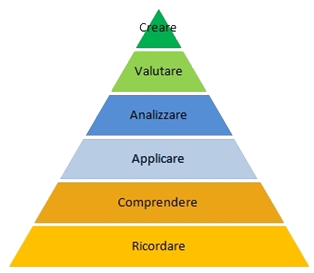
\includegraphics[height=5.4cm]{./immagini/01_Cap1/TassonomiaBloom}
	\caption{Piramide di Bloom revisionata da Anderson}
\end{figure}


Dagiene \textit{et al.} \cite{DagieneKEYCIT2015} declinano la tassonomia di Bloom rivista da Anderson nell'ambito dei quesiti Bebras proponendo il seguente elenco:
\begin{itemize}
	\item \textbf{Ricordare} 
	\begin{itemize}
		\item ricordare fatti generali, concetti di base
	\end{itemize}
	\item \textbf{Comprendere} 
	\begin{itemize}
		\item comprendere (livello facile) un dato linguaggio e il significato di comandi dati
		\item comprendere (livello complesso) la descrizione di processi, di regole di comportamento e di metodi
	\end{itemize}
	\item \textbf{Applicare} 
	\begin{itemize}
		\item applicare regole generative o metodi ad uno stato iniziale, a un input o una situazione
		\item interpretare istruzioni o programmi dati
	\end{itemize}
	\item \textbf{Analizzare}
	\begin{itemize}
		\item analizzare situazioni e processi
		\item abbinare descrizioni con i relativi comportamenti
	\end{itemize}
	\item \textbf{Valutare}
	\begin{itemize}
		\item confrontare diverse situazioni o soluzioni in base a criteri dati
		\item dedurre un possibile risultato, uno stato finale o un prodotto finale
	\end{itemize}
	\item \textbf{Creare} 
	\begin{itemize}
		\item mettere insieme informazioni
	\end{itemize}
\end{itemize}

Questa classificazione considera un aspetto molto interessante: le abilità coinvolte nella risoluzione dei quesiti Bebras ma presenta alcune criticità.
Si può osservare che la prima categoria è difficilmente applicabile ai quesiti in quanto non è mai richiesta volutamente una conoscenza pregressa.
Inoltre il punto ``Creare'' è descritto come ``mettere insieme informazioni'': definizione che non evoca in sé un processo creativo, e di cui gli autori non esplicitano un'interpretazione né forniscono esempi di quesiti Bebras di questo tipo, mentre esistono sicuramente quesiti Bebras che richiedono un processo creativo, ad esempio quelli in cui è chiesta la stesura di codice.



Tra tutte le classificazioni esposte in questa sezione solo quella bidimensionale proposta da Dagiene \textit{et al.} \cite{DagieneINFORMATICA2017} nel 2017 introduce una novità nello scopo della classificazione: non si vuole solo ottenere una distribuzione uniforme dei quesiti Bebras ma anche creare delle categorie comprensibili da docenti di qualsiasi formazione affinché i quesiti possano diventare uno strumento didattico all'interno del curricolo scolastico.
Con questo scopo nel Capitolo 3 verrà approfondito il tema del pensiero computazionale e come quest'ultimo possa rappresentare una chiave di lettura dei quesiti Bebras come risorsa didattica.
%
%
%			CAPITOLO 2: Indicazioni nazionali e Bebras
\chapter{Indicazioni nazionali e Bebras}
\label{cap2}
%%%%%%%%%%%%
\section{L'informatica nella scuola italiana}
%
Il termine informatica ha diverse accezioni:  Mirolo \cite{Mirolo2003} distingue tre approcci culturali sostanzialmente diversi che convergono in questo termine.
L'informatica è una \textit{scienza}: fornisce particolari chiavi di lettura con cui interpretare la realtà e specifici approcci alla risoluzione di problemi. 
L'informatica è intesa anche come \textit{tecnologia}, orientata a capire le caratteristiche, la struttura e i principi di funzionamento dei dispositivi hardware e software basati sulle tecnologie informatiche. 
Infine l'informatica è considerata uno \textit{strumento} per affrontare problemi che emergono in contesti diversi. Quest'ultimo è l'aspetto più diffuso in ambito scolastico dove vengono proposte iniziative tipicamente focalizzate su questo aspetto strumentale dell'informatica.


L'introduzione dell'informatica nel sistema scolastico italiano ha inizio negli anni '80 con l’utilizzo dei primi personal computer nelle scuole. In quegli anni vengono sviluppate pionieristiche iniziative di avvio alla programmazione e uso delle tecnologie informatiche. Nell'anno scolastico 1986/87 nella secondaria di secondo grado si avviano i vari Piani Nazionali per l’Informatica che introducono basi di programmazione e linguaggi informatici come ausilio per l'apprendimento di discipline quali matematica e fisica, mentre nella scuola primaria si diffonde Logo, un linguaggio di programmazione ideato da Papert, come strumento didattico finalizzato alla manipolazione di concetti geometrici.
Successivamente, l'evoluzione di hardware e software ha reso sempre più facile l'interazione con i computer ed ha portato ad un conseguente cambiamento nel modo di concepire e usare la tecnologia digitale in ambito scolastico. Gradualmente si è passati da un interesse formativo centrato sull'applicazione di elementi e metodi propri dell'informatica nei programmi scolastici delle altre discipline ad un approccio volto allo sviluppo di metodi e pratiche basate sull'uso delle Tecnologie dell'Informazione e della Comunicazione (TIC) per migliorare e innovare i processi di insegnamento nei vari ambiti disciplinari. Comincia quindi a diffondersi prepotentemente l'accezione dell'informatica come uso delle applicazioni, in particolare attraverso i corsi organizzati nelle scuole riguardanti l'alfabetizzazione digitale e l'acquisizione di certificati come l'ECDL.


Bellettini \textit{et al.} in \cite{BellettiniTOCE2014} rilevano alcuni punti critici del sistema italiano che rallentano la diffusione dell'insegnamento dell'informatica come disciplina scientifica: i docenti responsabili dell'introduzione dell'informatica nella scuola primaria non hanno necessariamente una laurea informatica, i libri di testo si concentrano principalmente sugli aspetti tecnologici e strumentali ad esempio sull'utilizzo di elaboratori ed infine è ancora forte la percezione dell'informatica come solo utilizzo del computer quindi spesso i genitori richiedono alla scuola l'alfabetizzazione digitale piuttosto che la comprensione delle questioni informatiche.

Dall'entrata in vigore nel 1999 dell'autonomia scolastica, gli Istituti scolastici ogni tre anni redigono un documento che presenta i percorsi didattici che devono rispettare le indicazioni e gli obiettivi fissati a livello nazionale dal Ministero dell'Istruzione. Per la scuola dell'infanzia, primaria e secondaria di primo grado il documento di riferimento sono le ``Indicazioni nazionali per il curricolo della scuola dell'infanzia e del primo ciclo d'istruzione'' \cite{indicazioniNazionali}.
% INFORMATICA ALLE ELEMENTARI %
Nella scuola primaria l'insegnamento dell'Informatica non ha delle ore dedicate: spesso vengono inserite alcune ore di laboratorio in cui gli studenti sono introdotti all'informatica attraverso l'uso del computer, quindi l'informatica intesa come strumento.
% INFORMATICA ALLE MEDIE %
Nella scuola secondaria di primo grado la situazione non è molto diversa: nonostante ci siano dei riferimenti più espliciti all'informatica all'interno della materia ``Tecnologia'' nella realtà l'insegnamento di tale disciplina si focalizza sull'uso del computer.

Per quanto riguarda la scuola secondaria di secondo grado, la situazione è diversa: esistono degli indirizzi specifici per lo studio dell'informatica. I documenti di riferimento per i Licei sono le ``Indicazioni nazionali'' \cite{IndicazioniLicei} mentre agli Istituti Tecnici e Professionali sono fornite le ``Linee guida'' \cite{IndicazioniIstituti}.
Per l'indirizzo “Opzione scienze applicate” del Liceo Scientifico si delinea un percorso da svolgere in 2 ore settimanali in tutti gli anni in cui i temi trattati sono architetture hardware, sistemi operativi, algoritmi e linguaggi di programmazione, reti e database.
Per gli Istituti Professionali gli obiettivi previsti riguardano per lo più l'uso delle applicazioni dell'informatica, riferendosi in particolare agli ambiti della grafica e della multimedialità.
Negli Istituti Tecnici del settore economico è prevista una materia denominata ``Informatica'' mentre in quelli del settore tecnologico ``Tecnologie informatiche''. In entrambi i casi i contenuti scelti sono orientati a formare una professionalità spendibile immediatamente nel mondo del lavoro.


Nel prossimo paragrafo si evidenzierà come nelle indicazioni ministeriali per il primo ciclo è possibile trovare nessi con aspetti fondamentali dell'informatica che hanno valore formativo generale nonostante non sia presente l'informatica come materia curricolare.
%%%%%%%%%%%%
\section{L'informatica nelle indicazioni nazionali per la scuola}
\label{indicazioni}
Le indicazioni nazionali per il curricolo della scuola dell'infanzia e del primo ciclo d’istruzione \cite{indicazioniNazionali} sono un testo di riferimento che sostituisce i Programmi Ministeriali utilizzati fino al 2004.
Nella parte introduttiva del documento viene presentato il concetto di \textit{centralità della persona}: al docente non è richiesta la trasmissione di concetti fini a se stessi, ma si vuole porre lo studente al centro dell'azione formativa; gli insegnanti sono invitati a pensare e realizzare i progetti didattici non in astratto ma partendo ogni anno dai ragazzi delle classi a cui sono stati assegnati.
Nelle Indicazioni viene inoltre riportato il quadro delle competenze-chiave per l’apprendimento, definite dal Parlamento Europeo e dal Consiglio dell'Unione Europea, che il sistema scolastico italiano assume come orizzonte di riferimento verso cui tendere.
Nella seconda parte del documento si entra nel merito delle indicazioni per la scuola dell'infanzia e per la scuola del primo ciclo che è composta da primaria e secondaria di primo grado.
Per ogni area disciplinare sono indicati i \textit{traguardi per lo sviluppo delle competenze} e gli \textit{obiettivi di apprendimento}: i primi sono riferimenti che indicano \textit{piste didattiche} da percorrere e costituiscono i criteri per la valutazione delle competenze attese, i secondi sono organizzati in \textit{nuclei tematici} e individuano conoscenze e abilità ritenuti indispensabili al fine di raggiungere le competenze individuate.

Abbiamo svolto un'attenta analisi delle Indicazioni Nazionali per verificare l'eventuale presenza di nessi con la disciplina informatica, anche se questa non è prevista come specifica materia di insegnamento.
Quest'analisi ha evidenziato che in alcuni casi ci sono dei riferimenti all'informatica intesa come utilizzo della tecnologia mentre spesso si trovano collegamenti ``nascosti'' all'informatica come scienza: alcuni traguardi e obiettivi di diverse aree disciplinari descrivono competenze e abilità che possono essere acquisite attraverso lo studio dell'informatica.
L'intero elenco dei traguardi e obiettivi ritenuti affini all'informatica è riportato nell'Appendice \ref{ElencoIndicazioni}.

Un esempio di riferimento esplicito all'informatica con l'accezione di strumento è il seguente traguardo rivolto a studenti della primaria: ``\textit{Usa manuali delle discipline o testi divulgativi nelle attività di studio personali e collaborative, per ricercare, raccogliere e rielaborare dati, informazioni e concetti; costruisce sulla base di quanto letto testi o presentazioni con l’utilizzo di strumenti tradizionali e informatici}''. In Tecnologia tra gli obiettivi per la secondaria si legge: ``\textit{Accostarsi a nuove applicazioni informatiche esplorandone le funzioni e le potenzialità}''.

Altri riferimenti espliciti si trovano in Tecnologia e riguardano il tema della programmazione: sia nella parte introduttiva dell'area disciplinare ``\textit{Quando possibile, gli alunni potranno essere introdotti ad alcuni linguaggi di programmazione particolarmente semplici e versatili che si prestano a sviluppare il gusto per l’ideazione e la realizzazione di progetti (siti web interattivi, esercizi, giochi, programmi di utilità) e per la comprensione del rapporto che c’è tra codice sorgente e risultato visibile}'' sia tra gli obiettivi rivolti alla scuola secondaria ``\textit{Programmare ambienti informatici e elaborare semplici istruzioni per controllare il comportamento di un robot}''.

La visione dell'informatica come materia scientifica non è mai esplicitamente espressa ad eccezione dei riferimenti alla programmazione appena citati. Altre tematiche come gli algoritmi e la loro complessità, la rappresentazione dei dati e il \textit{problem solving} non vengono mai introdotti esplicitamente; nonostante ciò, in particolar modo nelle prefazioni di alcune aree disciplinari, si indica al docente l'acquisizione di metodi di ragionamento tipici dell'informatica. 
Ad esempio nella parte introduttiva di Matematica si legge: ``\textit{Gradualmente, stimolato dalla guida dell'insegnante e dalla discussione con i pari, l’alunno imparerà ad affrontare con fiducia e determinazione situazioni problematiche, rappresentandole in diversi modi, conducendo le esplorazioni opportune, dedicando il tempo necessario alla precisa individuazione di ciò che è noto e di ciò che s’intende trovare, congetturando soluzioni e risultati, individuando possibili strategie risolutive}''.
Affrontare i problemi in questo modo è un comportamento tipicamente informatico che richiede di individuare le informazioni utili, organizzarle in adeguate strutture che aiutano ad ideare una strategia risolutiva e la successiva analisi e verifica delle possibili soluzioni. 
``\textit{Nella scuola secondaria di primo grado si svilupperà un’attività più propriamente di matematizzazione, formalizzazione, generalizzazione. L’alunno analizza le situazioni per tradurle in termini matematici, riconosce schemi ricorrenti, stabilisce analogie con modelli noti, sceglie le azioni da compiere e le concatena in modo efficace al fine di produrre una risoluzione del problema. Un’attenzione particolare andrà dedicata allo sviluppo della capacità di esporre e di discutere con i compagni le soluzioni e i procedimenti seguiti.}''. 
Purtroppo parte di queste indicazioni, espresse nelle prefazioni delle varie aree disciplinari, non vengono approfondite nella successiva stesura dei traguardi e degli obiettivi.



\bigskip
\textit{Descrizione di procedimenti}

\noindent Numerosi nessi con l'informatica sono presenti in Matematica e Tecnologia, essendo le materie più affini, ma anche in aree disciplinari idealmente lontane, come Italiano o Musica, si rilevano obiettivi e traguardi che possono essere promossi attraverso l'insegnamento dell'informatica. Ad esempio nell'informatica è fondamentale che la descrizione delle istruzioni sia precisa e non ambigua affinché ad un dato input o situazione si ottenga il risultato atteso.
Si trovano, a tal riguardo, riferimenti nell'area disciplinare di Tecnologia sia nella scuola primaria, dove un obiettivo è ``\textit{Realizzare un oggetto descrivendo e documentando la sequenza di azioni}'', sia nella scuola secondaria di primo grado nel traguardo ``\textit{Sa utilizzare comunicazioni procedurali e istruzioni tecniche per eseguire, in maniera metodica e razionale, compiti operativi complessi, anche collaborando e cooperando con i compagni}''.
Riferimenti riguardanti questa tematica si rilevano anche in vari obiettivi di Italiano, ad esempio ``\textit{Seguire istruzioni scritte per realizzare prodotti, per regolare comportamenti, per svolgere un'attività, per realizzare un procedimento}''. In quest'ultimo esempio non vi è un riferimento diretto all'informatica ma la descrizione che viene richiesta è la stessa che si sviluppa affrontando argomenti tipicamente informatici come lo studio o l'ideazione di algoritmi e procedure.


\bigskip
\textit{Problem solving}

\noindent In informatica il \textit{problem solving} è fondamentale: a partire da una condizione data si vuole risolvere un problema formalizzandolo e scegliendo il modo migliore per risolverlo. A tal riguardo nelle Indicazioni Nazionali si trova un traguardo per la scuola secondaria di primo grado nell'area disciplinare di Matematica: ``Confronta procedimenti diversi e produce formalizzazioni che gli consentono di passare da un problema specifico a una classe di problemi''.

\bigskip
\textit{Rappresentazione delle informazioni}

\noindent Un altro tema tipicamente informatico è la rappresentazione delle informazioni, cioè l'utilizzo di simboli, grafici o tabelle per la descrizione dei dati contenuti nell'informazione stessa. Ci sono diversi aspetti riguardanti questa tematica: affinché un'informazione possa essere elaborata automaticamente da un sistema informatico è necessario che sia rappresentata in un linguaggio di programmazione, inoltre la rappresentazione grafica e l'utilizzo di una specifica struttura rendono spesso più chiara l'informazione stessa e facilitano eventuali decisioni da prendere.
In Matematica ad esempio si indica, tra i traguardi della scuola secondaria, l'uso e l'interpretazione del linguaggio matematico per la descrizione di informazioni: tradurre concetti, fatti e operazioni dal linguaggio naturale in un linguaggio non ambiguo; questa abilità si sviluppa anche affrontando problemi informatici, infatti è necessario tradurre i passi da svolgere in istruzioni non ambigue che possono essere elaborate automaticamente. Anche nell'area disciplinare di Musica si trova un obiettivo per la primaria riguardante questo tema ed in partiolare l'aspetto della codifica, cioè la traduzione di informazioni in simboli: ``\textit{Rappresentare gli elementi basilari di brani musicali e di eventi sonori attraverso sistemi simbolici convenzionali e non}''. In Tecnologia si evidenzia l'aspetto della rappresentazione tramite tabelle o grafici, infatti ci sono diversi riferimenti alla comprensione e osservazione di mappe, diagrammi e disegni che, come accennato, sono rappresentazioni utili e spesso necessarie per la comprensione delle informazioni a disposizione.

\bigskip
\textit{Organizzazione dei dati}

\noindent L'organizzazione dei dati in base alle loro proprietà è fondamentale sia per la scelta della struttura dati più adatta alla circostanza sia per poter elaborare nel migliore dei modi i dati a disposizione. Questo processo non è importante solo nell'ambito scientifico ma è un'abilità richiesta anche in altre aree, infatti uno dei traguardi di Storia per la scuola primaria è: ``\textit{Usa la linea del tempo per organizzare informazioni, conoscenze, periodi e individuare successioni, contemporaneità, durate, periodizzazioni}''.

\bigskip
\textit{Pattern, regolarità, modelli}

\noindent La capacità di organizzare adeguatamente i dati a disposizione permette più facilmente il riconoscimento di pattern e similitudini, che è un processo fondamentale in informatica, ad esempio nel lavoro con un database è necessario riconoscere le proprietà significative e comuni in un insieme di oggetti per poter formulare una query.
Nell'area disciplinare della Matematica spesso si fa riferimento a questo tema; per la scuola primaria vengono riportati il seguente obiettivo: ``\textit{Riconoscere e descrivere regolarità in una sequenza di numeri o di figure}''.
L'abilità di rilevare similitudini e pattern in un insieme di oggetti è importante anche perché è un processo propedeutico all'astrazione e alla generalizzazione attraverso cui è possibile la creazione di modelli applicabili su un insieme di oggetti simili. A tal riguardo tra i traguardi di Scienze per la scuola secondaria si rileva: ``\textit{Sviluppa semplici schematizzazioni e modellizzazioni di fatti e fenomeni ricorrendo a semplici formalizzazioni}''.

\bigskip
\textit{Metodo sperimentale}

\noindent L'informatica, come tutte le altre discipline scientifiche, propone allo studente un approccio con il metodo sperimentale: un programma è l'ipotesi di partenza, questo deve essere eseguito, testato e successivamente modificato nel caso in cui il risultato ottenuto non corrisponde all'ipotesi di partenza.
Il metodo scientifico basato su ipotesi e sperimentazioni viene proposto in un traguardo per la scuola primaria nell'area disciplinare di Scienze: ``\textit{Esplora i fenomeni con un approccio scientifico: osserva e descrive lo svolgersi dei fatti, formula domande, anche sulla base di ipotesi personali, propone e realizza semplici esperimenti}''.
Fondamentale, in questo approccio scientifico, è la capacità di sostenere le proprie idee formulando ragionamenti e confrontandosi con punti di vista diversi: spesso nell'ambito informatico è richiesto il lavoro di squadra e il confronto per il raggiungimento della soluzione migliore. A tal riguardo nell'area disciplinare di Matematica è riportato il seguente traguardo rivolto alla scuola secondaria: ``\textit{Sostiene le proprie convinzioni, portando esempi e controesempi adeguati e utilizzando concatenazioni di affermazioni; accetta di cambiare opinione riconoscendo le conseguenze logiche di una argomentazione corretta}''.



\bigskip
Questa analisi ha fatto emergere quali nessi si possono trovare tra le indicazioni proposte dal Ministero e i temi tipici dell'informatica; riteniamo quindi che molte abilità e competenze indicate come fondamentali per la formazione dell'individuo sono assimilabili anche attraverso la disciplina informatica. Per facilitare, ciò nel paragrafo successivo, abbiamo pensato di verificare l'esistenza di almeno un quesito Bebras per ogni indicazione affine all'informatica.

%%%%%%%%%%%%
\section{Relazione tra Bebras e Indicazioni Nazionali} \label{classIndicazioni}

I quesiti Bebras possono rappresentare una risorsa didattica per veicolare contenuti e metodi informatici sotto forma di gioco. Affinché essi possano essere utilizzati in maniera adeguata in relazione alle tematiche presentate in classe, abbiamo fatto un lavoro di corrispondenza tra le Indicazioni Nazionali e i quesiti proposti nelle edizioni italiane delle gare.

Si può notare come la forma dei giochi Bebras sono coerenti con le indicazioni del Ministero.
Nella parte introduttiva dell'area disciplinare di Matematica, ad esempio, si legge: ``\textit{Caratteristica della pratica matematica è la risoluzione di problemi, che devono essere intesi come questioni autentiche e significative, legate alla vita quotidiana, e non solo esercizi a carattere ripetitivo o quesiti ai quali si risponde semplicemente ricordando una definizione o una regola}''. I quesiti Bebras possiedono esattamente le caratteristiche riportate: si tratta spesso di problemi riconducibili a questioni significative legate alla vita quotidiana in cui la logica ricopre un ruolo fondamentale, non è mai richiesto di ricordare a memoria l’uso di definizioni o di regole ma tutte le informazioni necessarie a risolvere il problema dato sono contenute nel testo.
Inoltre, come visto nel Capitolo 1, le gare Bebras in Italia vengono proposte come attività da svolgere in squadre per il raggiungimento della soluzione, così da far maturare la necessità di confronto e di discussione con i compagni. A tal proposito nelle Indicazioni si trova: ``\textit{Un’attenzione particolare andrà dedicata allo sviluppo della capacità di esporre e di discutere con i compagni le soluzioni e i procedimenti seguiti}''. 

Oltre all'individuazione di questi riferimenti più generici, abbiamo fatto un lavoro sistematico di ricerca di corrispondenze tra i quesiti Bebras e le Indicazioni Nazionali: per ogni punto dei traguardi e degli obiettivi affini all'Informatica è stato cercato almeno un quesito che possa avvicinare lo studente a contenuti e metodi informatici sotto forma di gioco.

Il risultato ottenuto da questa analisi è stato riportato in una tabella: le righe riportano i traguardi e gli obiettivi delle Indicazioni Nazionali affini all'informatica suddivisi per area didattica e grado scolastico, mentre le colonne riportano il titolo di alcuni quesiti Bebras in cui si è rilevato un nesso con almeno un'indicazione.
Alcuni traguardi e obiettivi sono stati scomposti in più punti per rendere la corrispondenza più specifica.
Si riportano di seguito due frammenti della tabella ottenuta: la corrispondenza tra i quesiti Bebras e i traguardi (Figura 11) e gli obiettivi (Figura 12) dell'area disciplinare di Matematica nella scuola primaria.
Si può notare che esistono molte corrispondenze tra le indicazioni fornite dal Ministero e i quesiti Bebras. Per questo motivo riteniamo importante che i quesiti possano essere integrati all'interno del curricolo e presentati in classe come spunto di partenza per un nuovo argomento, un'esercitazione o un approfondimento.
Di seguito verranno proposti alcuni quesiti Bebras come esempi del lavoro svolto.

\begin{figure}[H]
	\centering
	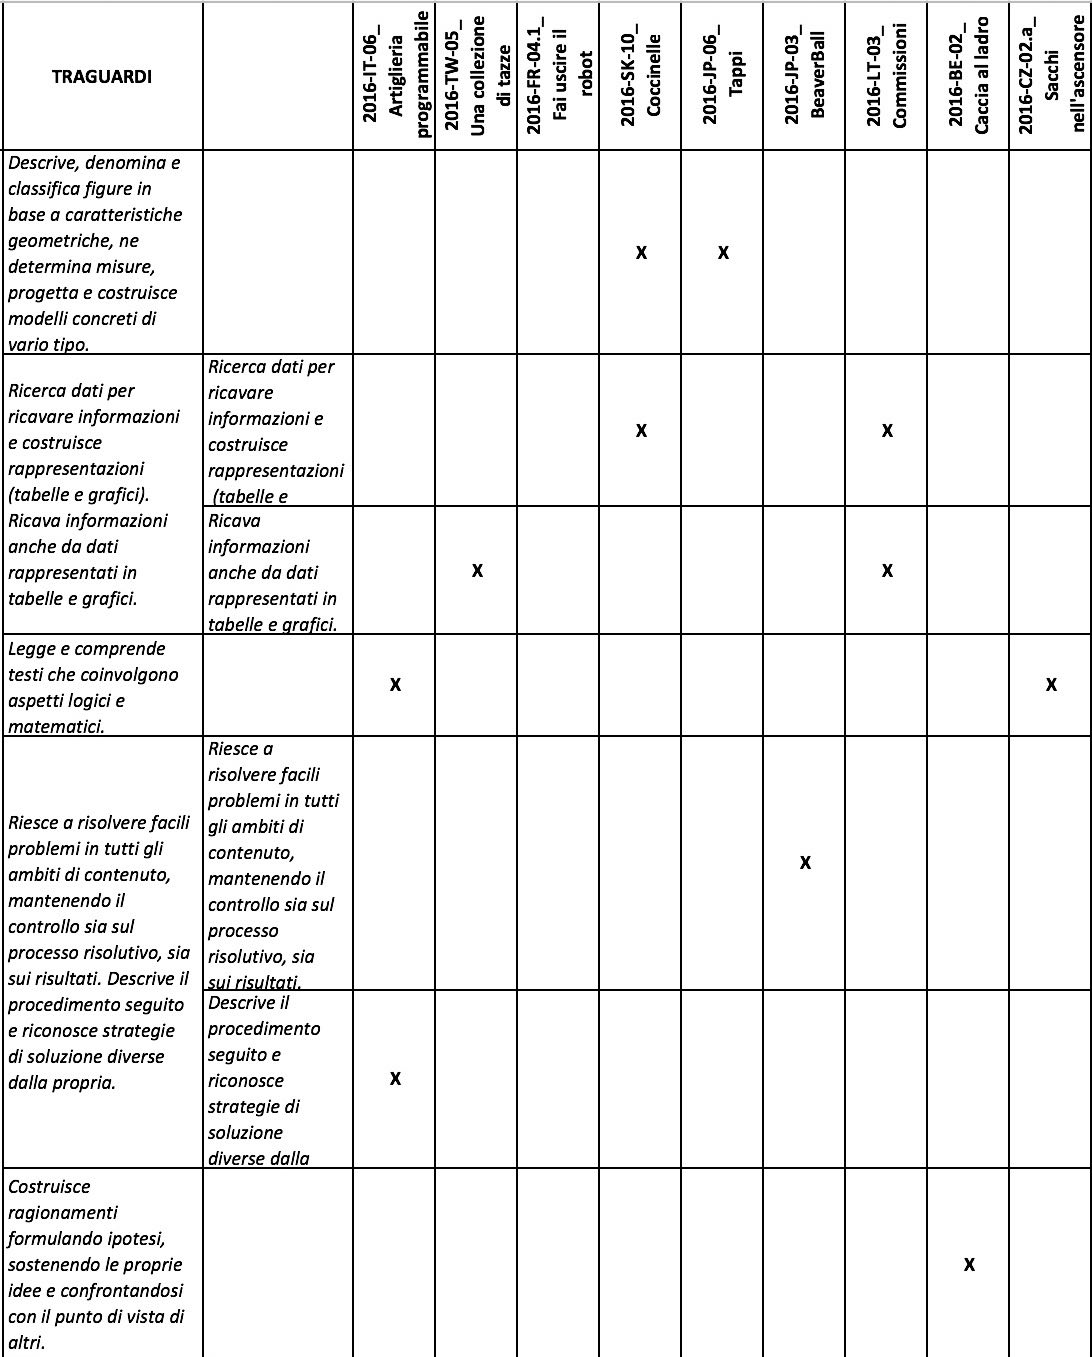
\includegraphics[width=15.0cm]{./immagini/02_Cap2/TabellaMatchIndicazioniMate} \label{indicazioniMatematica}
	\caption{Corrispondenze tra i quesiti Bebras e i traguardi di Matematica nella scuola primaria}
\end{figure}

\begin{figure}[H]
	\centering
	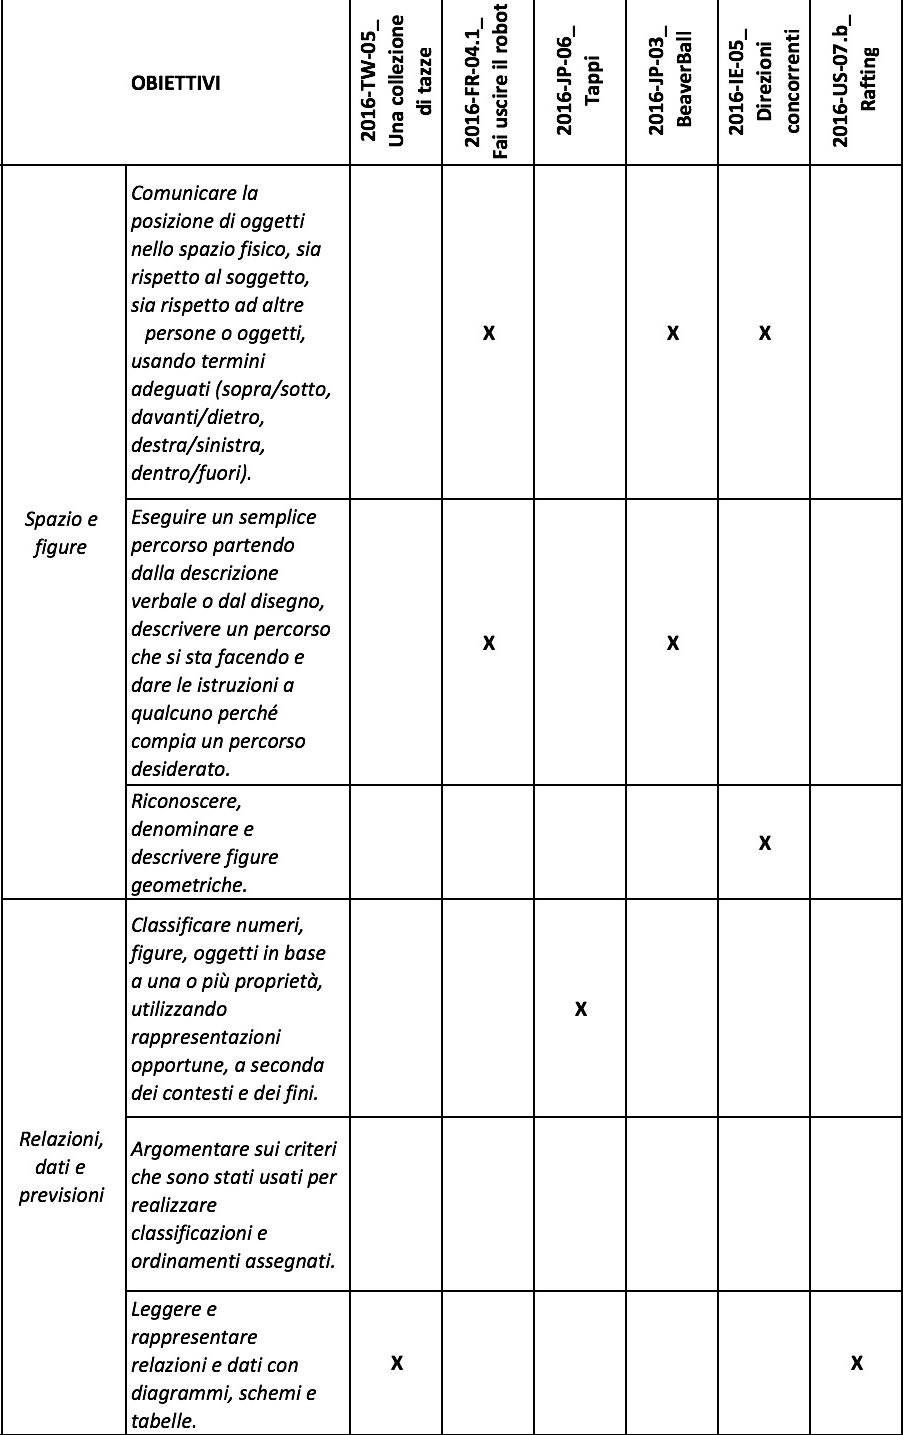
\includegraphics[width=13.0cm]{./immagini/02_Cap2/MatchObiettiviMate}
	\caption{Corrispondenze tra i quesiti Bebras e gli obiettivi di Matematica alla fine della classe terza della scuola primaria}
\end{figure}


\newpage
Il quesito ``Commissioni'' (Figura \ref{fig:corrispondenze1}), creato dal gruppo lituano nel 2016 e proposto in Italia nelle categorie KiloBebras e MegaBebras, presenta un tipico problema di pianificazione o \textit{scheduling} che consiste nel determinare l'ordine corretto o ottimale in cui eseguire un insieme di azioni. Una delle attività principali nel mondo informatico è la ricerca delle soluzioni ammissibili, caratterizzate dal fatto di soddisfare uno o più vincoli: nel nostro caso i vincoli sono legati al visitare un luogo solo dopo che se ne è visitato un altro.
Il quesito in questione si può riferire al seguente traguardo della scuola primaria nell'area disciplinare di Matematica:
``\textit{Ricerca dati per ricavare informazioni e costruisce rappresentazioni (tabelle e grafici). Ricava informazioni anche da dati rappresentati in tabelle e grafici}''.
Lo studente, per trovare l'ordine corretto delle commissioni, deve ricavare dalla tabella data le informazioni riguardanti il tempo necessario per l'esecuzione di ogni operazione da eseguire e le ore di punta da evitare. Una possibile strategia risolutiva è quella di creare a sua volta una tabella (Figura \ref{fig:corrispondenze2}) in cui indicare sulle righe le attività e la loro relativa durata mentre sulle colonne le possibili fasce orarie.


\begin{figure}[H]
	\centering
	\fbox{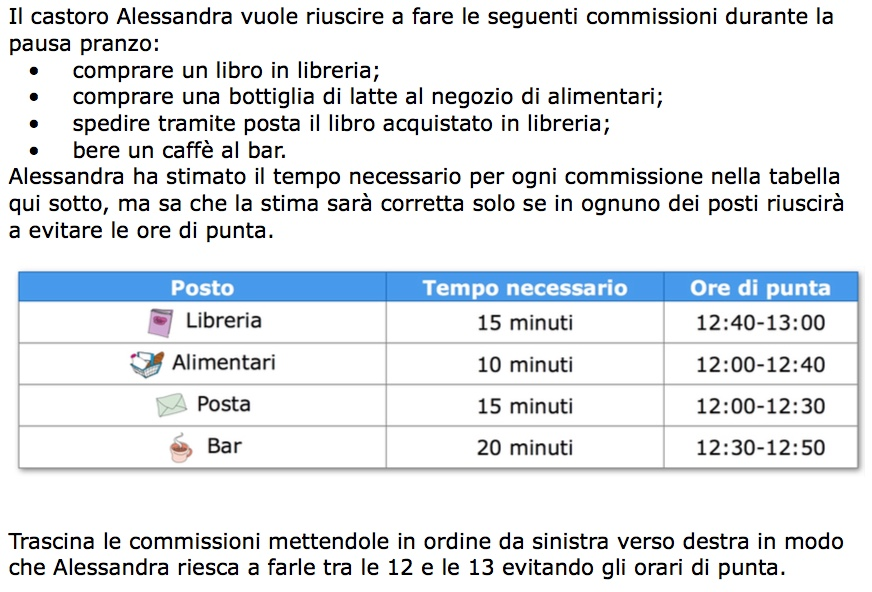
\includegraphics[width=15.0cm]{./immagini/02_Cap2/corrispondenze1}}
	\caption{``Commissioni'' quesito Bebras dell'edizione italiana 2016 per le categorie KiloBebras e MegaBebras}\label{fig:corrispondenze1}
\end{figure}

\begin{figure}[H]
	\centering
	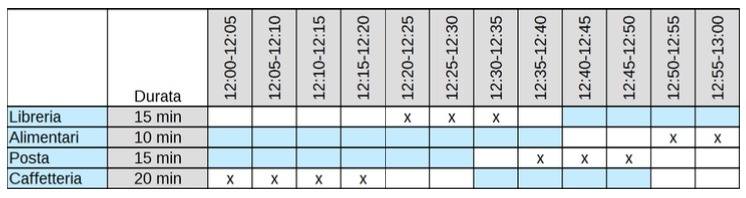
\includegraphics[width=15.0cm]{./immagini/02_Cap2/corrispondenze2}
	\caption{Esempio tabella di supporto per la risoluzione del quesito ``Commissioni''}\label{fig:corrispondenze2}
\end{figure}

Per quanto riguarda la scuola secondaria di primo grado nell'area didattica di Matematica si possono trovare altri traguardi pertinenti:
``\textit{Analizza e interpreta rappresentazioni di dati per ricavarne misure di variabilità e prendere decisioni}'', ``\textit{Riconosce e risolve problemi in contesti diversi valutando le informazioni e la loro coerenza}''.
Lo studente deve interpretare la tabella proposta nel testo e dedurne le informazioni necessarie alla richiesta, inoltre deve valutare la compatibilità tra i vari eventi indicati per poterne decidere l'ordine.
Un possibile approfondimento didattico, successivo allo svolgimento del quesito, è spiegare la costruzione della tabella da cui ricavare la soluzione e confrontare la strategia risolutiva proposta con quelle scelte dalle varie squadre partecipanti, incentivando in questo modo il confronto tra procedure e approcci diversi.

Un altro obiettivo dell'area disciplinare di Matematica è: ``\textit{Riconoscere coppie di eventi complementari, incompatibili, indipendenti}'' che è strettamente riconducibile allo scopo del quesito, infatti allo studente è richiesto di ordinare gli eventi e quindi riconoscere che tipo di relazione intercorre tra di essi.
Anche nell'area disciplinare di Scienze è possibile rintracciare dei riferimenti utili:
``\textit{Individua nei fenomeni somiglianze e differenze, fa misurazioni, registra dati significativi, identifica relazioni spazio/temporali}'', infatti il processo risolutivo del quesito chiede allo studente di riconoscere le relazioni temporali tra gli eventi proposti.



\bigskip
\begin{figure}[h]
	\centering
	\fbox{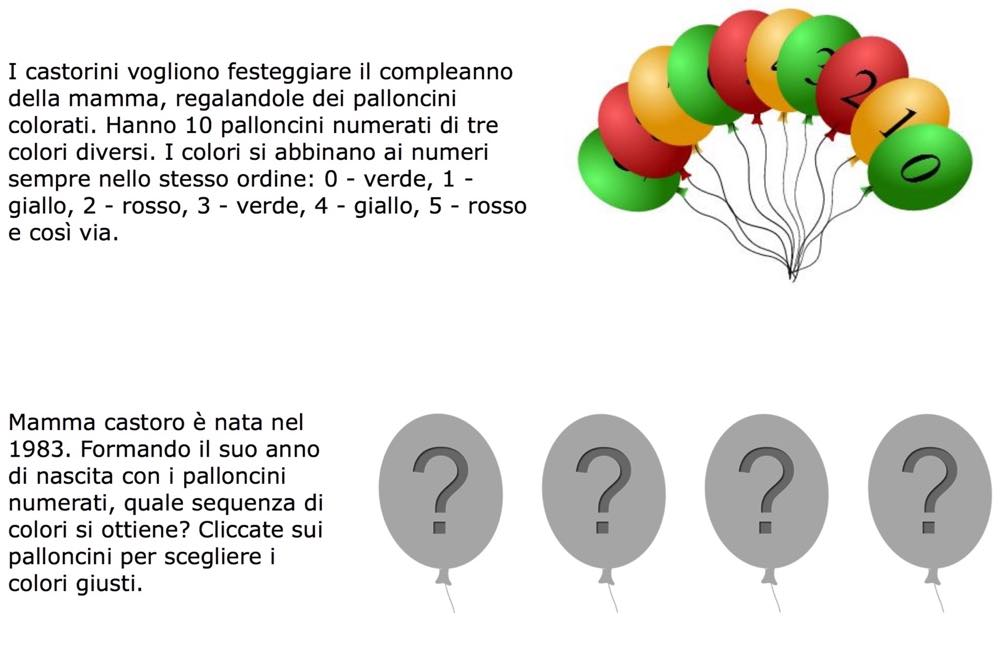
\includegraphics[width=15.0cm]{./immagini/02_Cap2/palloncini}}
	\caption{``Palloncini'' quesito Bebras dell'edizione italiana 2015 per la categoria KiloBebras}\label{fig:palloncini}
\end{figure}

Il quesito ``Palloncini'' (Figura \ref{fig:palloncini}) è stato ideato dal gruppo Bebras della Turchia e proposto in Italia nel 2015 agli studenti della scuola primaria. Il quesito richiede sia abbinamenti tra numeri e colori che l'ordinamento di oggetti per la rappresentazione dell'informazione.
Infatti si deve tradurre l'informazione dell'anno della nascita della mamma castoro in una sequenza di colori, questa attività di codifica si può ritrovare nelle Indicazioni Nazionali sia tra i traguardi di Musica: ``\textit{Decodificare e utilizzare la notazione tradizionale e altri sistemi di scrittura}'' sia in Matematica in cui è richiesta la traduzione di concetti dal linguaggio naturale in un linguaggio non ambiguo. Questo quesito può essere un pretesto per notare la differenza tra linguaggio ambiguo e non, infatti la sequenza finale dei colori dei palloncini rappresenta l'informazione di partenza non in maniera univoca.



\bigskip
\begin{figure}[h]
	\centering
	\fbox{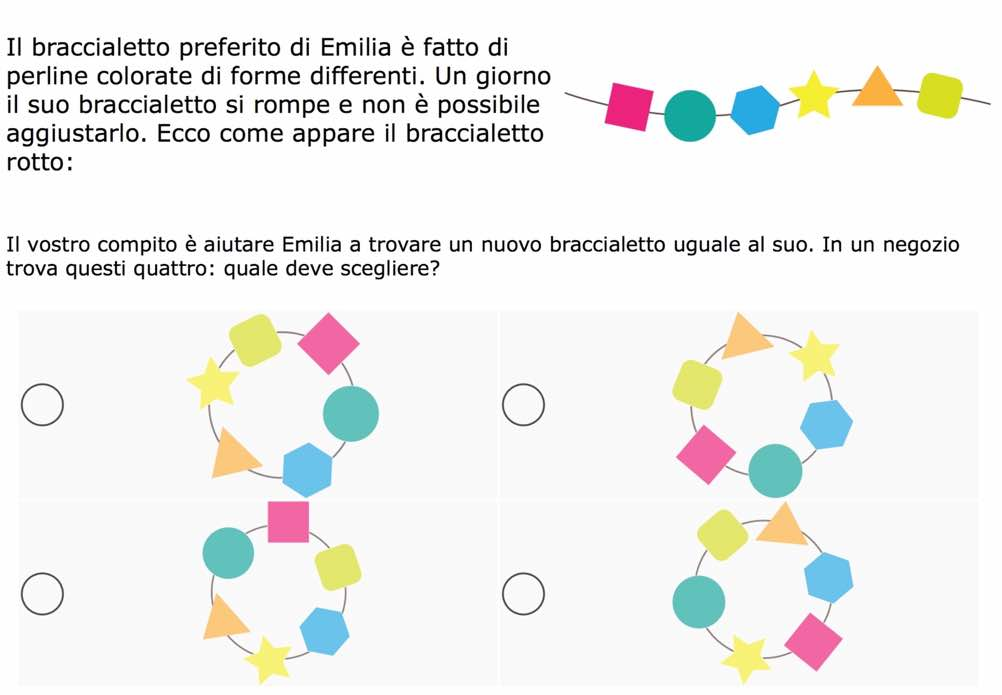
\includegraphics[width=15.0cm]{./immagini/02_Cap2/braccialetti}}
	\caption{``Braccialetti'' quesito Bebras dell'edizione italiana 2015 per la categoria KiloBebras}\label{fig:braccialetti}
\end{figure}

Il quesito ``Braccialetti'' (Figura \ref{fig:braccialetti}), proposto nel 2015 dal gruppo Bebras della Malesia, ideato per i bambini della scuola primaria, chiede di riconoscere quale delle quattro ipotesi proposte corrisponde all'ordine corretto degli oggetti. Nelle Indicazioni Nazionali, come già detto nella precedente sezione, si trovano diversi riferimenti all'acquisizione di questa abilità di riconoscimento di similitudini soprattutto nell'ambito matematico. Rispetto al quesito proposto, ad esempio, è evidente che ci sia un nesso con gli obiettivi dell'area disciplinare di Matematica ``\textit{Riconoscere figure ruotate, traslate e riflesse}'' e ``\textit{Riconoscere e descrivere regolarità in una sequenza di numeri o di figure}''. L'ordinamento delle perline, infatti, identifica uno schema che deve essere cercato in tutti i braccialetti: saper riconoscere schemi può aiutare a trovare delle similitudini tra cose che a prima vista sembrano diverse ma che invece hanno qualcosa in comune infatti, quando si realizza che un compito è simile ad un altro già affrontato precedentemente, è possibile applicare un metodo simile per svolgere il nuovo
compito.

\bigskip

\begin{figure}[h]
	\centering
	\fbox{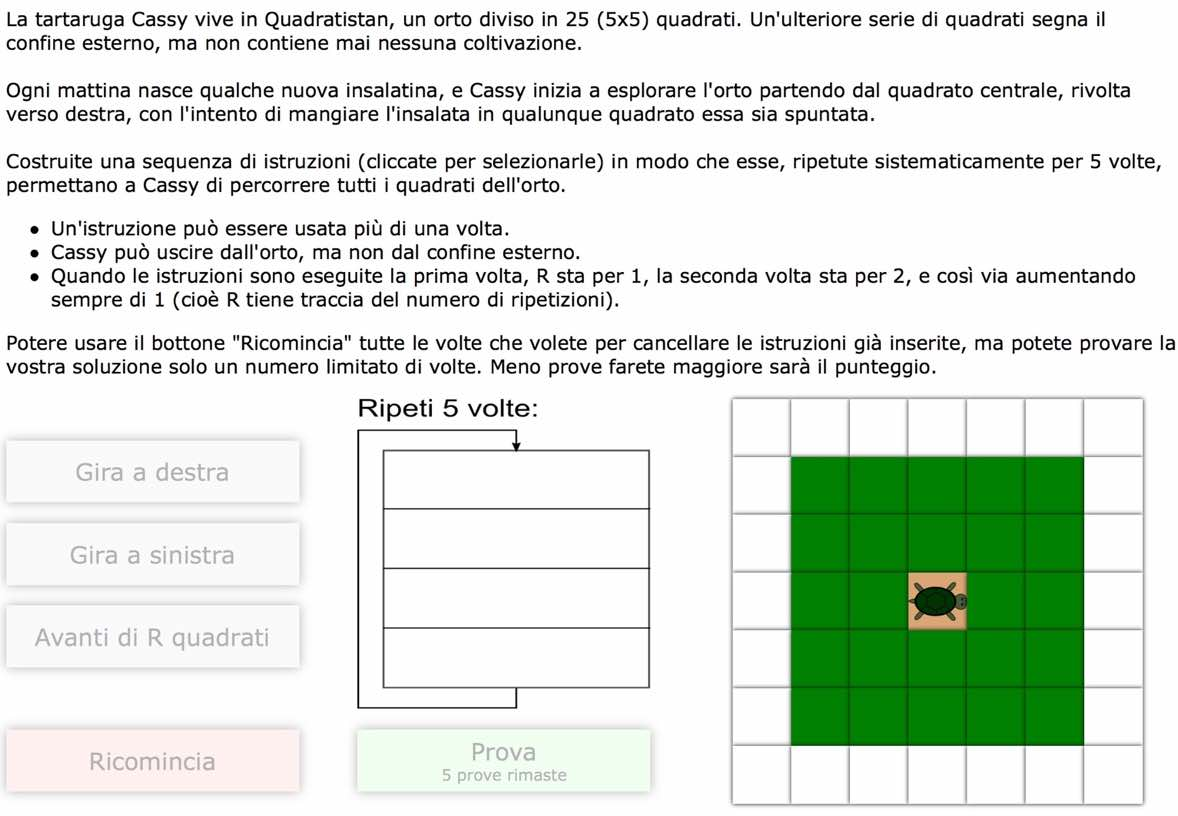
\includegraphics[width=15.0cm]{./immagini/02_Cap2/tartaruga}}
	\caption{``Una tartaruga sistematica'' quesito Bebras dell'edizione italiana 2016 per le categorie MegaBebras, GigaBebras e TeraBebras}\label{fig:tartaruga}
\end{figure}

Nel quesito ``Una tartaruga sistematica'' (Figura \ref{fig:tartaruga}) si richiede di scrivere un programma attraverso la giustapposizione delle istruzioni che vengono fornite; viene anche data la possibilità di verificare il programma creato grazie all'interattività del 	quesito e quindi, nel caso di errori, lo studente può modificare e testare nuovamente il proprio programma. Questo quesito è rivolto ai ragazzi della scuola secondaria di primo grado ed è evidentemente orientato all'introduzione della programmazione con una sintassi molto semplificata. Nella scuola secondaria i docenti sono invitati ad introdurre gli aspetti basilari della programmazione nell'area disciplinare di Tecnologia sia tra i traguardi ``\textit{Progetta e realizza rappresentazioni grafiche o infografiche, relative alla struttura e al funzionamento di sistemi materiali o immateriali, utilizzando elementi del disegno tecnico o altri linguaggi multimediali e di programmazione}'', sia tra gli obiettivi ``\textit{Programmare ambienti informatici e elaborare semplici istruzioni per controllare il comportamento di un robot}''.
Inoltre è possibile trovare in questo quesito anche l'aspetto informatico fondamentale dell'individuazione di una strategia adeguata per il raggiungimento dell'obiettivo finale: lo studente, prima di poter costruire la sequenza di istruzioni, dovrà riflettere su quale strada far percorrere alla tartaruga affinché visiti tutti i quadrati dell'orto. A tal riguardo nelle Indicazioni Nazionali, nella parte introduttiva dell'area disciplinare di Matematica, si trova: ``\textit{(...) l’alunno imparerà ad affrontare con fiducia e determinazione situazioni problematiche (...) individuando possibili strategie risolutive}''.


\bigskip
\begin{figure}[h]
	\centering
	\fbox{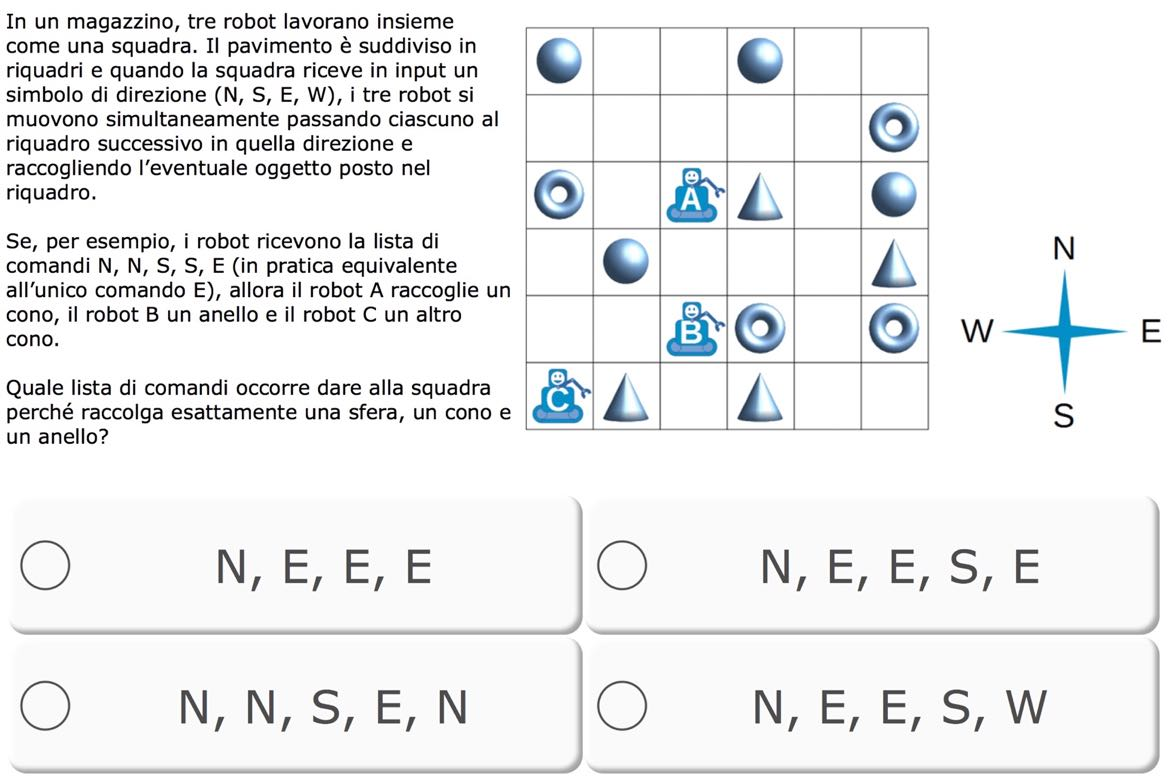
\includegraphics[width=15.0cm]{./immagini/02_Cap2/direzioni}}
	\caption{``Direzioni concorrenti'' quesito Bebras dell'edizione italiana 2016 per le categorie KiloBebras, MegaBebras e GigaBebras}\label{fig:direzioni}
\end{figure}

``Direzioni concorrenti'' (Figura \ref{fig:direzioni}) è un quesito ideato dal gruppo Bebras Irlanda e proposto nell'edizione italiana del 2016. Questo quesito presenta allo studente il concetto di esecuzione parallela di più istruzioni: in informatica è fondamentale scomporre un problema in sotto-problemi che possano essere risolti contemporaneamente in maniera indipendente. Nel caso proposto i tre robot eseguono la stessa sequenza di comandi e lo studente deve fare attenzione affinché ognuno di essi raggiunga l'oggetto richiesto senza urtare il bordo del riquadro.
Il quesito proposto ha diversi riferimenti rintracciabili nelle Indicazioni Nazionali, ad esempio un obiettivo dell'area disciplinare di Matematica per la scuola primaria è ``\textit{Comunicare la posizione di oggetti nello spazio fisico, sia rispetto al soggetto, sia rispetto ad altre persone o oggetti, usando termini adeguati (sopra/sotto, davanti/dietro, destra/sinistra, dentro/fuori)}'': lo studente infatti, nella risoluzione del quesito, deve sia confrontarsi con i simboli di direzione sia saperli utilizzare adeguatamente. 


%%%%%%%%%%%%
%			CAPITOLO 3: CT e Bebras
\chapter{Il computational thinking e i quesiti Bebras}
\label{cap3}
%%%%%%%%%
\section{Il pensiero computazionale}
% spiegazione del CT e riportare le operazioni del volantino del ciste
La locuzione \textit{computational thinking} (pensiero computazionale) è stata usata per la prima volta da Seymour Papert nel 1996 in \cite{PapertCT} parlando di educazione matematica con il suo linguaggio di programmazione didattico Logo. 
Nel 2006 il concetto di pensiero computazionale è stato riportato in primo piano da Jeannette Wing in un articolo \cite{WingCT2006} in cui afferma che lo sviluppo del pensiero computazionale è indispensabile per tutti, non solo per gli addetti al settore informatico, e che è un'abilità che può essere usata nella vita di tutti i giorni. La Wing afferma che bisognerebbe aggiungere il pensiero computazionale come abilità da insegnare ad ogni bambino: l'invenzione della stampa ha permesso la diffusione delle tre abilità di base cioè leggere, scrivere e calcolare, allo stesso modo la diffusione della tecnologia deve permettere la diffusione del pensiero computazionale.


La definizione di pensiero computazionale proposto da Nardelli in \cite{NardelliCT} è:
``\textit{Il pensiero computazionale è un processo mentale per far risolvere problemi ad un agente, sia esso persona o macchina, fornendogli una serie di istruzioni che deve eseguire in autonomia}''.
Con \textit{processo mentale} si specifica la sua indipendenza da tecnologie, strumenti concreti e sistemi fisici. Il termine \textit{agente} sta ad indicare chi esegue le istruzioni e si evidenzia il suo essere distinto rispetto al soggetto in cui avviene il processo mentale.
In altre parole il pensiero computazionale è il ``pensare come un informatico'' quando si affronta un problema.


Per permettere più facilmente la definizione di obiettivi educativi e la loro valutazione, l'ISTE (International Society for Technology in Education) e la CSTA (Computer Science Teachers Association) hanno redatto, insieme ad alcuni docenti, una definizione operazionale del pensiero computazionale \cite{flayerCT}. Il pensiero computazionale è un processo per la risoluzione di problemi che utilizza le seguenti operazioni:
\begin{enumerate}[label=(\alph*)]
	\item formulare il problema in un formato che ci permette di usare un ``sistema di calcolo'' (nel senso più ampio del termine, ovvero una macchina, un essere umano, o una rete di umani e macchine) per risolverlo;
	\item analizzare e organizzare logicamente i dati del problema;
	\item rappresentare i dati del problema tramite opportune astrazioni, modelli e simulazioni;
	\item automatizzare la risoluzione del problema definendo una soluzione algoritmica, che consista in una sequenza accuratamente descritta di passi;
	\item identificare, analizzare, implementare e testare le possibili soluzioni con un'efficace ed efficiente combinazione di passi e risorse, avendo come obiettivo la ricerca della soluzione migliore secondo tali criteri;
	\item generalizzare il processo di problem solving per poterlo trasferire ad un ampio spettro di problemi.
\end{enumerate}

Il pensiero computazionale sviluppa la capacità di progettare soluzioni di un dato problema ad esempio collezionando dati e analizzandoli, scomponendo il problema in sotto-problemi o ancora creando algoritmi.
Parte fondamentale di questo \textit{pensiero informatico} è implementare i progetti programmando e automatizzando la soluzione che successivamente deve essere testata ed eventualmente modificata. Un'altra competenza che si acquisisce attraverso lo studio dell'informatica è la discussione delle proprie ipotesi risolutive con il team di lavoro, avendo quindi la capacità di presentare e comunicare i propri risultati.



Le competenze discusse sono sostenute ancora di più dalle seguenti attitudini \cite{attitudiniCT}:
\begin{itemize}
	\item confidenza nel trattare la complessità;
	\item perseveranza nell'affrontare problemi difficili;
	\item tolleranza per l'ambiguità;
	\item saper fronteggiare problemi aperti;
	\item saper comunicare e lavorare con gli altri per raggiungere un obiettivo o una soluzione comune;
	\item conoscere i propri punti di forza e le proprie carenze quando si lavora con gli altri.
\end{itemize}

%%%%%%%%%%%%%%
\section{I quesiti Bebras descritti attraverso il pensiero computazionale} \label{ClassCT}
% articolo prof
I quesiti Bebras, come visto nel Capitolo 2, possono essere un ricco strumento per l'insegnamento curricolare dell'informatica e quindi, più in generale, per l'acquisizione del pensiero computazionale.
Per rendere esplicito il potenziale educativo dei quesiti Bebras anche a docenti privi di una formazione informatica, abbiamo descritto le abilità del pensiero computazionale, menzionate nella definizione operazionale, facendo riferimento a quesiti Bebras che possono promuovere tali abilità \cite{LonatiISSEP2017}.

\begin{itemize}
	\item \textbf{Organizzazione logica dei dati}: 
	\\
	I quesiti che tipicamente promuovono questa abilità riguardano l'organizzazione dei dati secondo certi criteri fissati con riferimenti, generalmente nascosti, ai database e alla teoria degli insiemi: possono chiedere di eseguire una query su una tabella che rappresenta un insieme di oggetti, di suddividere un insieme di elementi in categorie in base alle loro caratteristiche, o individuare un oggetto fuori luogo in una figura.
	Altri quesiti si concentrano sull'organizzazione dei dati in modo che godano di alcune proprietà: ad esempio la crittografia, in cui si vuole che un messaggio non sia comprensibile anche se intercettato, la compressione dei dati, dove si organizzano i dati in modo da trasmetterli e memorizzarli meglio, o la correzione di codici attraverso l'aggiunta di bit per rilevare o recuperare eventuali errori nella rappresentazione dei dati memorizzati o trasmessi.
	Rientrano in questa categoria anche quesiti in cui le strutture dati sono utilizzate per organizzare i dati per l'elaborazione. Ad esempio, un quesito può trattare l'uso di alberi di ricerca binari per trovare velocemente un elemento senza dover considerare l'intero insieme in cui è contenuto; altri possono trattare gli heap, le code, gli stack e così via. 
	Un esempio a tal riguardo è il quesito Bebras ``Sacchi nell'ascensore'' (Figura \ref{sacchi_ascensore}) in cui è necessario riuscire ad eseguire l'algoritmo descritto usando uno stack in modo che l'ultimo oggetto aggiunto sia sempre il primo a essere estratto.
	Se una struttura di dati viene utilizzata per rappresentare una proprietà intrinseca dei dati (ad esempio grafi per relazioni binarie, alberi per reazioni gerarchiche), il quesito viene classificato più adeguatamente all'interno della ``Rappresentazione digitale dell'informazione''.
	
		\begin{figure}[h]
		\centering
		\fbox{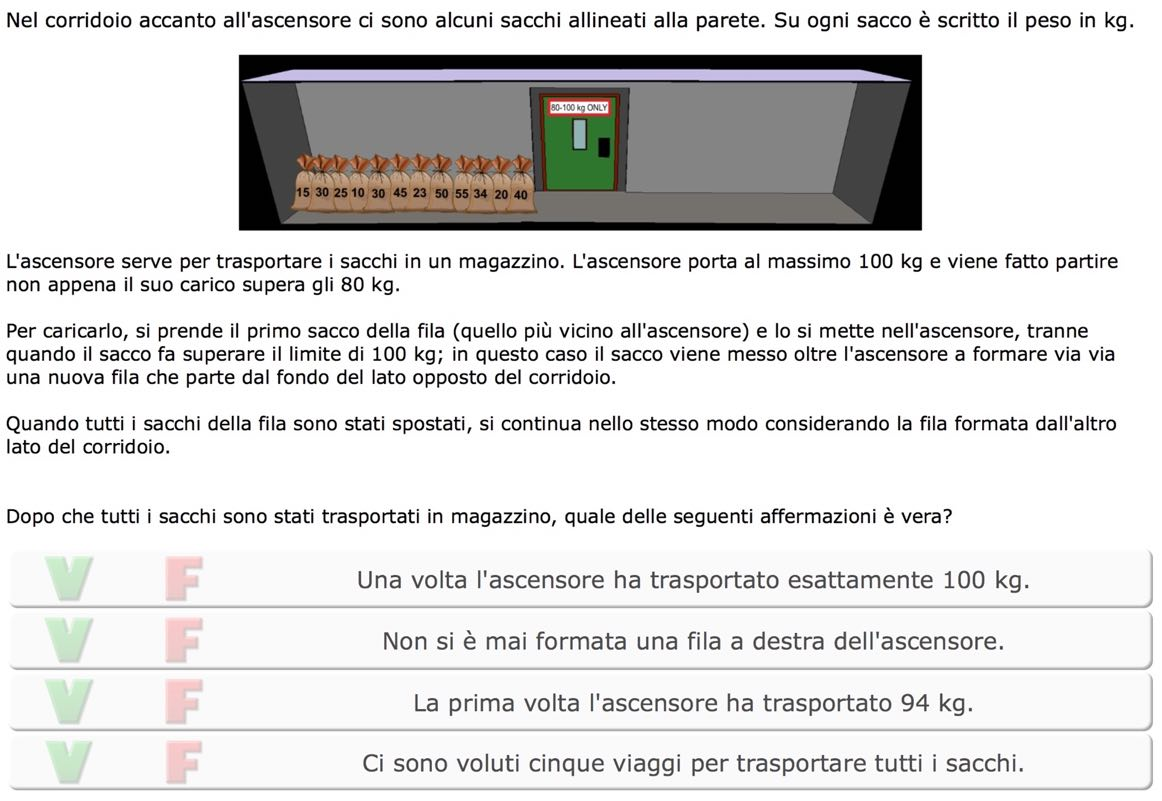
\includegraphics[width=15.0cm]{./immagini/03_Cap3/sacchi_ascensore}}
		\caption{``Sacchi nell'ascensore'' quesito Bebras dell'edizione italiana 2016 per le categorie KiloBebras, MegaBebras e GigaBebras}\label{sacchi_ascensore}
	\end{figure}

\bigskip	
	\item \textbf{Analisi logica dei dati}: 
	\\
	Molti quesiti in questa categoria sono percepiti come ``problemi logici'' perché richiedono inferenza logica, ragionamento deduttivo e di trarre conclusioni dai dati forniti.
	Altri quesiti chiedono di verificare se i dati del problema soddisfano certe proprietà che spesso non sono evidenti e per individuarle sono necessari alcuni ragionamenti ed osservazioni come il riconoscimento di pattern, o è necessario un approccio sistematico per raggiungere la giusta conclusione.
	Un esempio di questa tipologia di quesiti Bebras è quello proposto dalla delegazione della Repubblica Ceca nel 2015 (Figura \ref{2015-CZ-01}). Per risolvere questo quesito, lo studente deve astrarre le caratteristiche specifiche degli animali e considerare solo la loro struttura, quindi si possono mettere in corrispondenza le coppie di animali analizzando le loro proprietà come il numero di noci o il numero di connessioni da ciascuna noce.
	
	\begin{figure}[h]
		\centering
		\fbox{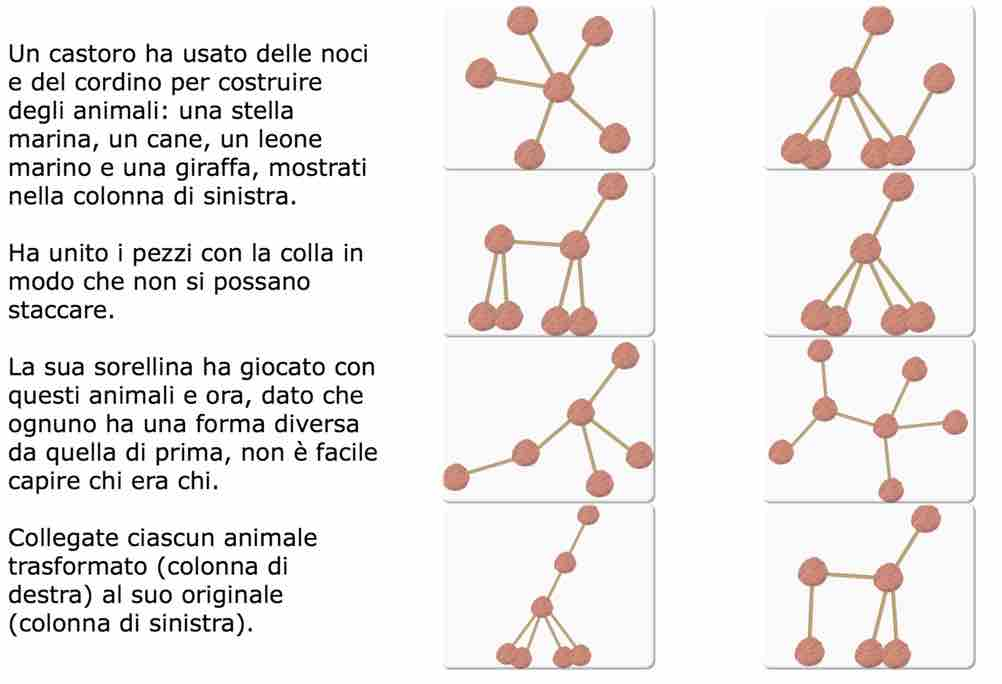
\includegraphics[width=15.0cm]{./immagini/03_Cap3/2015-CZ-01Testo}}
		\caption{``Noci e animali'' quesito Bebras dell'edizione italiana 2015 per le categorie KiloBebras, MegaBebras e GigaBebras}\label{2015-CZ-01}
	\end{figure}

\bigskip
	\item \textbf{Rappresentazione digitale dell'informazione}: 
	\\
	I quesiti di questa categoria riguardano la rappresentazione digitale dei numeri, delle immagini, più in generale di insiemi di oggetti, oppure la rappresentazione visiva di dati attraverso diagrammi come istogrammi o grafici.
	Altri quesiti introducono le strutture dati per rappresentare le proprietà rilevanti dei dati, come grafi per relazioni binarie o alberi per relazioni gerarchiche. Un esempio di quesito appartenente a questa categoria è quello proposto dalla delegazione Canadese nel 2015 (Figura \ref{2015-CA-01}), in cui viene utilizzato un grafo per rappresentare e visualizzare le relazioni d'amicizia tra le persone in un social network.
	
	\begin{figure}[h]
	\centering
	\fbox{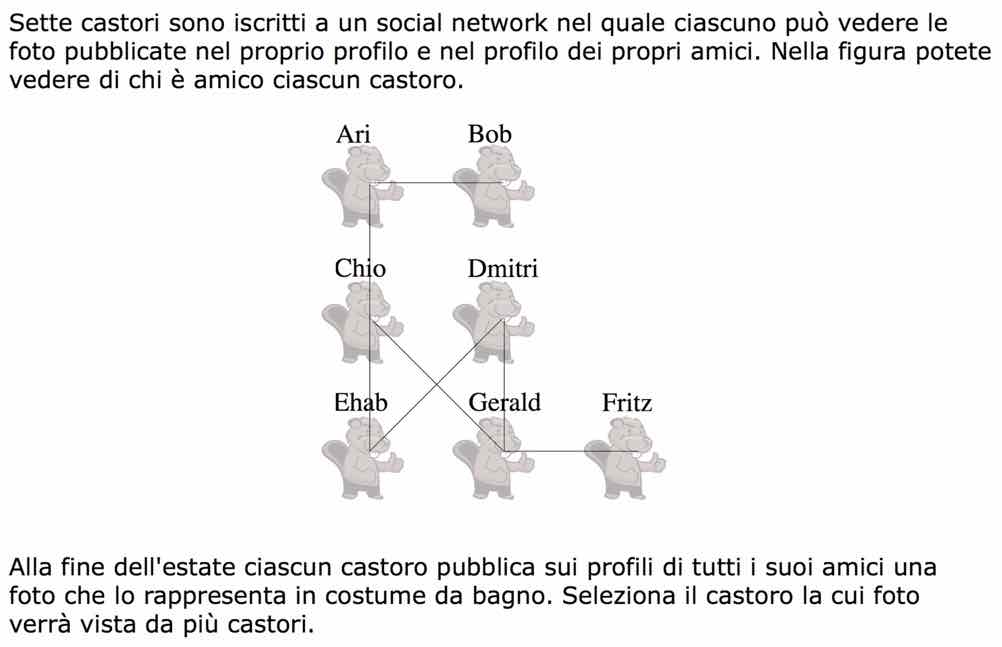
\includegraphics[width=15.0cm]{./immagini/03_Cap3/2015-CA-01Testo}}
	\caption{``Popolarità'' quesito Bebras dell'edizione italiana 2015 per le categorie GigaBebras, TeraBebras e PetaBebras}\label{2015-CA-01}
	\end{figure}
	
\bigskip
	\item \textbf{Pensiero algoritmico}: 
	\\
	Il pensiero algoritmico si occupa di trasformare un'intuizione in una forma adatta ad essere elaborata automaticamente. Quindi permette, ad esempio: di progettare un metodo sistematico per affrontare un problema a partire da un approccio intuitivo; di trasformare un'idea su come svolgere un compito in una procedura descritta passo per passo che raggiunge l'obiettivo; di dare una descrizione sintetica di una situazione o di un processo individuando e utilizzando i suoi pattern; di partire da una serie di esempi o da una descrizione informale e formalizzare una regola che può essere applicata in generale; e così via.
	Quindi, i quesiti appartenenti a tale categoria richiedono di manipolare i dati seguendo una procedura formale (ad esempio una sequenza di passi o mosse) o un insieme di regole o primitive come avviene nel quesito Bebras ``Labirinti intricati'' (Figura \ref{labirinti})
	Questi quesiti possono richiedere di eseguire alcune procedure o di calcolare o riconoscere l'output; di applicare alcune regole di transizione su un sistema in una data configurazione; di predire lo stato finale di un processo descritto tramite un diagramma (ad esempio un diagramma di transizione di un automa a stati finiti); di scomporre un problema in più parti; di combinare delle operazioni primitive per calcolare un risultato o di concludere un compito; di enumerare sistematicamente o esaminare tutti i possibili casi che possono presentarsi in un dato contesto; e così via.
	Si può notare che quando lo scopo del quesito riguarda l'implementazione (analisi o ideazione rispettivamente) di una soluzione algoritmica, allora il quesito si può posizionare più adeguatamente nella categoria ``Implementare soluzioni algoritmiche'' (``Analizzare soluzioni algoritmiche'' o ``Identificare strategie risolutive rispettivamente'').
	
	\begin{figure}[h]
		\centering
		\fbox{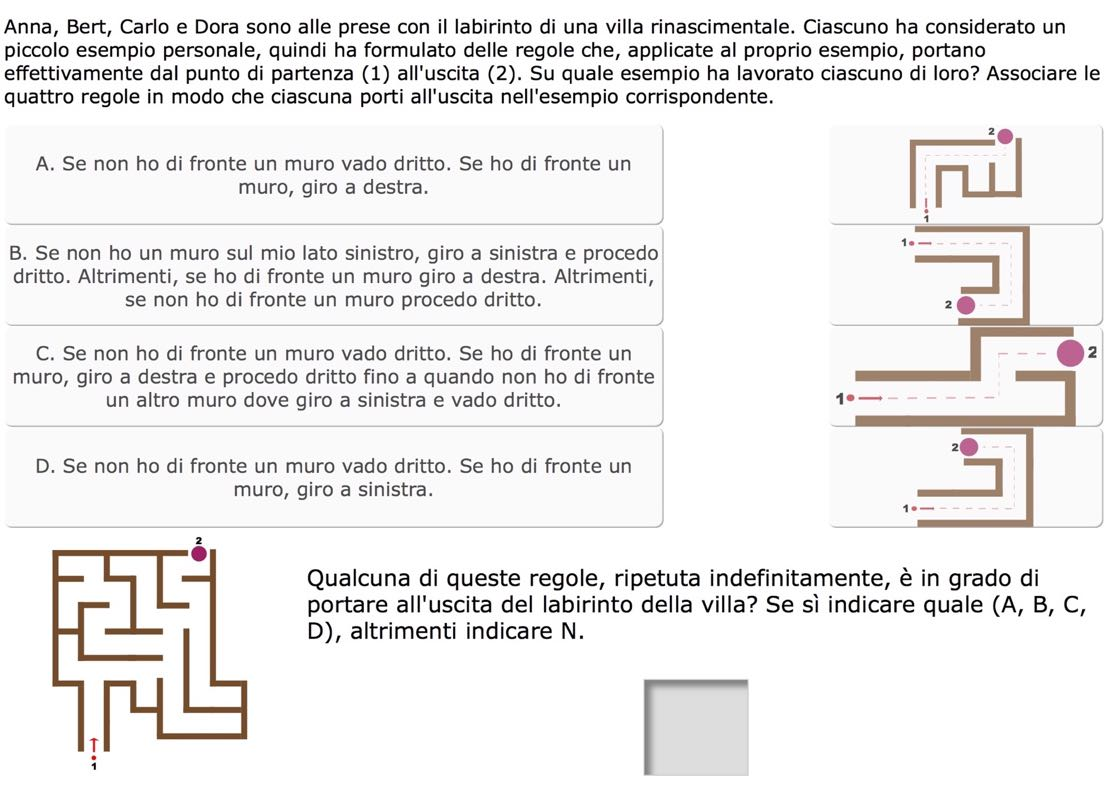
\includegraphics[width=15.0cm]{./immagini/03_Cap3/labirinti}}
		\caption{``Labirinti intricati'' quesito Bebras dell'edizione italiana 2015 per le categorie GigaBebras, TeraBebras e PetaBebras}\label{labirinti}
	\end{figure}


\bigskip
	\item \textbf{Identificare strategie risolutive}:
	\\
	Questa categoria riguarda la risoluzione dei problemi e in particolare la ricerca di una strategia algoritmica adeguata per affrontare un problema. In genere la formulazione di una soluzione algoritmica (in modo che possa essere automatizzata) non è sufficiente, i quesiti di questo insieme solitamente richiedono di avere un'idea non banale per affrontare il problema presentato.
	Un esempio è il quesito proposto dalla delegazione Belga nel 2016 (Figura \ref{2016-BE-02}), in cui viene chiesto di stimare il numero di interrogatori necessari per individuare il ladro, gli studenti devono intuire che un'analisi sequenziale di tutti i visitatori del museo richiede troppo tempo, è quindi necessario un approccio originale (in questo caso la ricerca binaria). 
	
	\begin{figure}[h]
		\centering
		\fbox{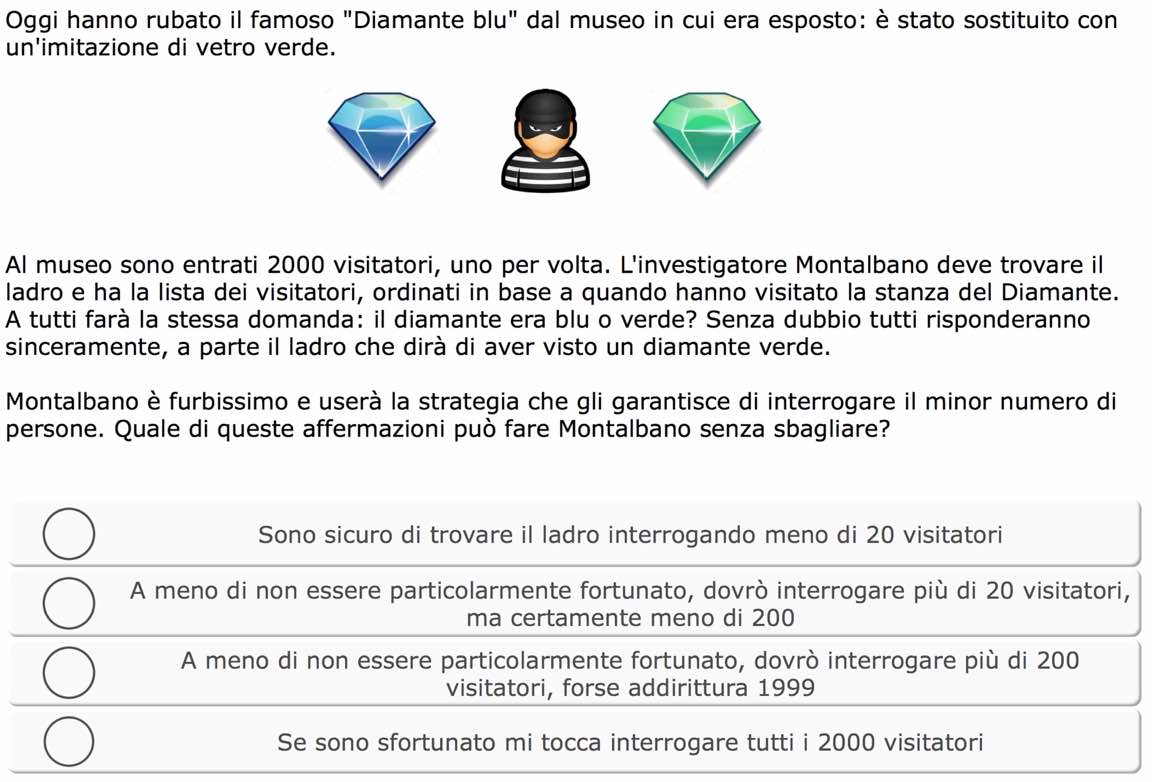
\includegraphics[width=15.0cm]{./immagini/03_Cap3/2016-BE-02Testo}}
		\caption{``Caccia al ladro'' quesito Bebras dell'edizione italiana 2016 per le categorie MegaBebras, GigaBebras e TeraBebras}\label{2016-BE-02}
	\end{figure}
	
\bigskip
	\item \textbf{Analizzare soluzioni algoritmiche}: 
	\\
	In questa categoria rientrano tutti i quesiti in cui si devono considerare le caratteristiche di un algoritmo come la correttezza o la complessità. Quindi si può richiedere di esaminare un algoritmo (o più in generale un metodo di calcolo) per capire la sua semantica, determinare le sue proprietà invarianti, stimare quante risorse consumerà. 
	Il quesito ``Artiglieria programmabile'' (Figura \ref{artiglieria_programmabile}) chiede di analizzare i risultati proposti e trovare il programma esatto al raggiungimento dell'obiettivo. 
	Inoltre sono compresi in questo insieme anche i quesiti ispirati a problemi di ottimizzazione in cui si richiede di confrontare e valutare diversi approcci per trovare il migliore.
	
	\begin{figure}[h]
		\centering
		\fbox{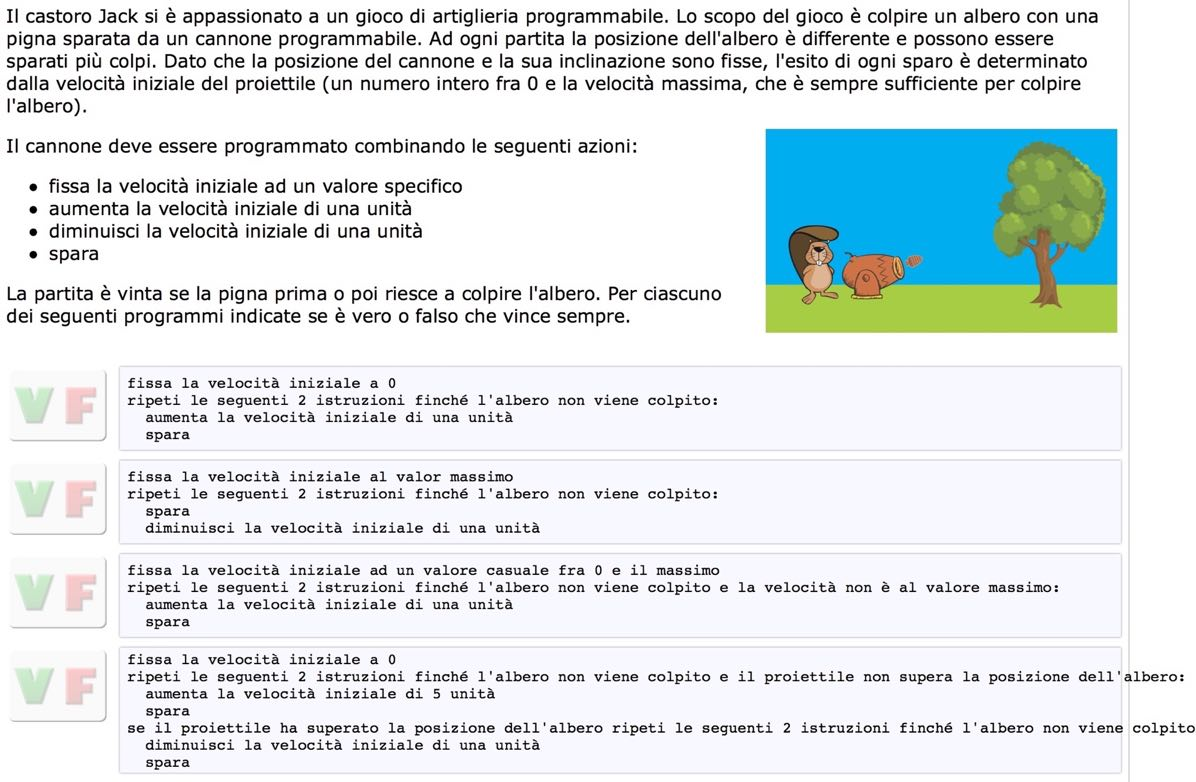
\includegraphics[width=15.0cm]{./immagini/03_Cap3/artiglieria_programmabile}}
		\caption{``Artiglieria programmabile'' quesito Bebras dell'edizione italiana 2016 per le categorie MegaBebras, GigaBebras e TeraBebras}\label{artiglieria_programmabile}
	\end{figure}
	
	
\bigskip
	\item \textbf{Implementare soluzioni algoritmiche}: 
	\\
	I quesiti appartenenti a questa categoria promuovono le attività di programmazione o codifica, l'attenzione è focalizzata sull'implementazione di algoritmi attraverso una sintassi formale definita nel quesito stesso. 
	Un esempio a tal riguardo è il quesito ``Fai uscire il robot'' (Figura \ref{robot}) in cui viene si richiede l'utilizzo di una struttura fondamentale per la programmazione, cioè il ciclo inteso come sequenza di istruzioni che viene ripetutamente eseguita fino al verificarsi di una data condizione.
	Nel caso in cui l'algoritmo da implementare non è semplice ma è necessario ideare una strategia di soluzione, allora il quesito farà parte anche delle categorie: ``Pensiero algoritmico'' e ``Identificare strategie risolutive''.
	
	\begin{figure}[h]
		\centering
		\fbox{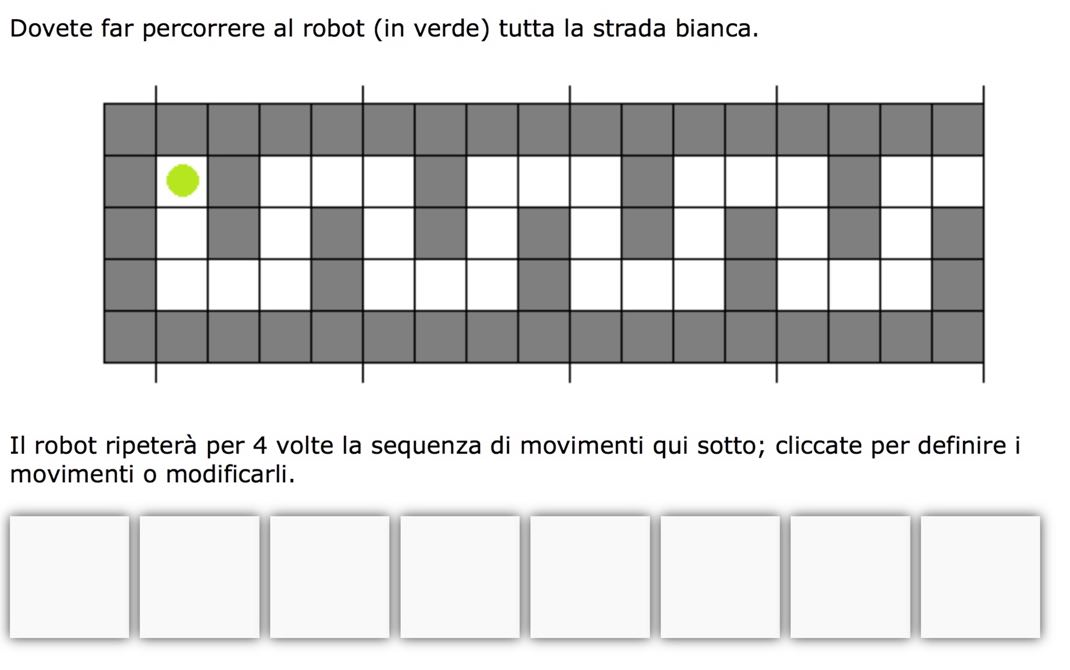
\includegraphics[width=15.0cm]{./immagini/03_Cap3/robot}}
		\caption{``Fai uscire il robot'' quesito Bebras dell'edizione italiana 2016 per le categorie KiloBebras, MegaBebras e GigaBebras}\label{robot}
	\end{figure}
	
\end{itemize}

%%%%%%%%%%
\section{Riscontri degli insegnanti} \label{interviste}
Descrivere i quesiti Bebras con riferimento alle abilità del pensiero computazionale (Sezione 2) ha lo scopo di evidenziare le potenzialità formative dei quesiti Bebras.
Abbiamo intervistato alcuni docenti con la tecnica dei \textit{key informant} per verificare se le descrizioni proposte sono prima di tutto comprensibili anche a chi non ha una formazione specifica in informatica e in secondo luogo se aiutano a comprendere come e in quali contesti utilizzare i quesiti Bebras nel curricolo scolastico.


La tecnica \textit{key informant} è una tecnica qualitativa che consiste nell'intervistare persone selezionate per la loro conoscenza approfondita dell'argomento di interesse. Le interviste si focalizzano su alcune tematiche specifiche che si vogliono affrontare, queste sono poco strutturate in modo da favorire un flusso libero di idee e informazioni, che successivamente vengono analizzate e rielaborate dagli intervistatori.
Nel nostro caso gli intervistati sono stati otto insegnanti in scuole di vari gradi, selezionati per la loro competenza e pratica riflessiva sulla didattica. Quattro di loro conoscevano già le gare Bebras o perché avevano avuto a che fare con i quesiti tramite le gare annuali oppure per il loro contributo alla preparazione dei quesiti stessi; l'altra metà degli intervistati sono insegnanti senza formazione o esperienza specifica in informatica ma interessati alle questioni curricolari e metodologiche riguardanti l'insegnamento.
A questi docenti abbiamo fornito una scheda, riportata di seguito, in cui si riporta una descrizione sintetica delle abilità del pensiero computazionale presentate nella Sezione 3.2; si chiede agli insegnanti di leggere attentamente le descrizioni e annotare eventuali dubbi o difficoltà di comprensione, in seguito si chiede di leggere alcuni quesiti Bebras, a loro scelta, disponibili sulla piattaforma di gara ed infine associare ognuno di essi ad una o più abilità descritte rispondendo alla domanda ``\textit{Usereste questo quesito per promuovere o insegnare questa capacità nell'ambito del pensiero computazionale?}''.


Nella stesura delle descrizioni riportate nella scheda abbiamo fatto particolare attenzione ad utilizzare un linguaggio meno tecnico possibile così da renderle comprensibili a tutti i docenti, indipendentemente dalla loro formazione.

\bigskip
\begin{comment}
\begin{framed}
\begin{center}
	\textbf{{\large Classificazione dei quesiti Bebras: una proposta basata sulla definizione di pensiero computazionale}}
\end{center}

\medskip
Ciascun quesito Bebras può essere esaminato considerando il suo valore didattico. Qui presentiamo sette tipi di quesiti, a partire da una definizione di Pensiero Computazionale.
Ti chiediamo gentilmente di:
\begin{itemize}
	\item leggere attentamente la descrizione dei tipi di quesito (che trovi di seguito) e annotare eventuali dubbi o difficoltà di comprensione
	\item leggere alcuni quesiti Bebras (ad esempio quelli dell'ultima edizione della gara, disponibili su \url{http://bebras.it/students})
	\item per ciascuno di questi quesiti, provare a rispondere alla domanda “Useresti questo quesito per promuovere o insegnare questa capacità nell'ambito del pensiero computazionale?”. Puoi rispondere compilando una tabella a doppia voce (quesito Bebras/categoria) assegnando ad ogni casella uno dei seguenti punteggi: 0=``assolutamente no''; 1=``più no che sì''; 2=``più sì che no''; 3=``assolutamente sì'' .
\end{itemize}

\bigskip
\begin{enumerate}
	\item \textbf{Organizzazione logica dei dati}
	\\
	I quesiti che rientrano tipicamente in questa classe trattano di: organizzazione dei dati secondo certi criteri fissati (come ad esempio in una tabella), uso di strutture per rendere i dati più facili da elaborare, organizzare i dati in modo che godano di proprietà interessanti come nel caso della crittografia (dove si vuole che un messaggio non sia comprensibile anche se intercettato) o della compressione dei dati (dove si organizzano i dati in modo che siano più facili da trasmettere o memorizzare).
	
	\item \textbf{Analisi logica dei dati}
	Qui si trovano quei ``problemi logici'' che si basano sul ragionamento logico-deduttivo e che chiedono di trarre conclusioni relative ai dati presentati nel quesito. Inoltre, in questa classe si trovano anche quesiti che richiedono di osservare attentamente gli oggetti coinvolti (es: per riconoscere elementi simili o ricorrenti) o di procedere in maniera sistematica per stabilire se i dati del problema soddisfano o meno certe proprietà.
	
	\item \textbf{Rappresentazione digitale delle informazioni}
	I quesiti tipici di questa classe hanno a che fare con la rappresentazione digitale/simbolica dei dati, o con la loro rappresentazione visuale tramite diagrammi come istogrammi o grafici. Altri quesiti fanno riferimento a strutture di dati che consentono di rappresentare proprietà interessanti (ad esempio: relazioni binarie o gerarchiche tra oggetti).

	\item \textbf{Pensiero algoritmico}
	I quesiti di questa classe chiedono di affrontare un problema attraverso l’uso di metodi sistematici o procedure passo-passo, andando oltre la pura idea intuitiva su come risolvere il problema. Ad esempio tramite la scomposizione del problema in sotto-problemi; la combinazione di operazioni elementari per svolgere un compito più complesso; l’uso di procedure formali (da eseguire o di cui calcolare/prevedere il risultato); l’applicazione di regole di transizione ad un sistema che si trova in un certo stato di partenza, ecc.
	
	\item \textbf{Identificare strategie risolutive}
	Il tema di questa classe è il problem solving e in particolare la ricerca di strategie algoritmiche non scontate per risolvere un problema.
	
	\item \textbf{Analizzare soluzioni algoritmiche}
	Questa classe contiene quesiti che riguardano le caratteristiche generali di un algoritmo o di un metodo risolutivo presentato nel quesito, quali la correttezza del metodo o la sua praticabilità. Altri quesiti tipici di questa classe sono quelli che si ispirano a problemi di ottimizzazione, in cui si cerca la soluzione “migliore” (es: più grande, meno costosa, più veloce, più breve, ecc) tra tutte le soluzioni accettabili.
	
	\item \textbf{Implementare soluzioni algoritmiche}
	I quesiti in questa classe possono essere pensati come problemi di programmazione o ``coding'', poiché si concentrano sull'implementazione di algoritmi attraverso l’uso di una sintassi formale definita nel quesito.
	
\end{enumerate}
\end{framed}
\end{comment}

\bigskip
Molti insegnanti intervistati hanno riposto alla scheda proposta compilando delle tabelle contenenti le corrispondenze tra i quesiti Bebras da loro scelti e le abilità del pensiero computazionale. A tal riguardo si riporta, come esempio, la tabella di risposta (Figura \ref{classificazione_insegnanti}) proposta da una docente di Matematica e Scienze di una scuola secondaria di primo grado. La docente intervistata inoltre ha ritenuto utile schematizzare a suo modo le descrizioni proposte (Figura \ref{rielaborazioneCT}).


In un secondo momento sono state analizzate le tabelle con le corrispondenze e abbiamo intervistato i docenti chiedendo loro di discutere le loro risposte per capire le loro motivazioni. Le interviste non erano strutturate con domande prestabilite, pur avendo l'obiettivo di approfondire questi temi:

\begin{enumerate}[label=(\arabic*)]
	\item Le descrizioni delle categorie sono comprensibili? Sono stati utilizzati termini o espressioni che non ha capito o che le sembrano ambigui? 
	
	\item Quali difficoltà ha riscontrato nell'associare i quesiti scelti con le descrizioni proposte?
	
	\item Perché ha associato un determinato quesito a tale categoria?
	
	\item Pensa che presentando i quesiti Bebras attraverso queste categorie presentate il valore formativo e didattico sia più evidente? Ovvero se i quesiti fossero presentati in questo modo sarebbe più facile per voi docenti utilizzarli come risorsa curricolare?
\end{enumerate}


\begin{figure}[htb]
	\centering
	\fbox{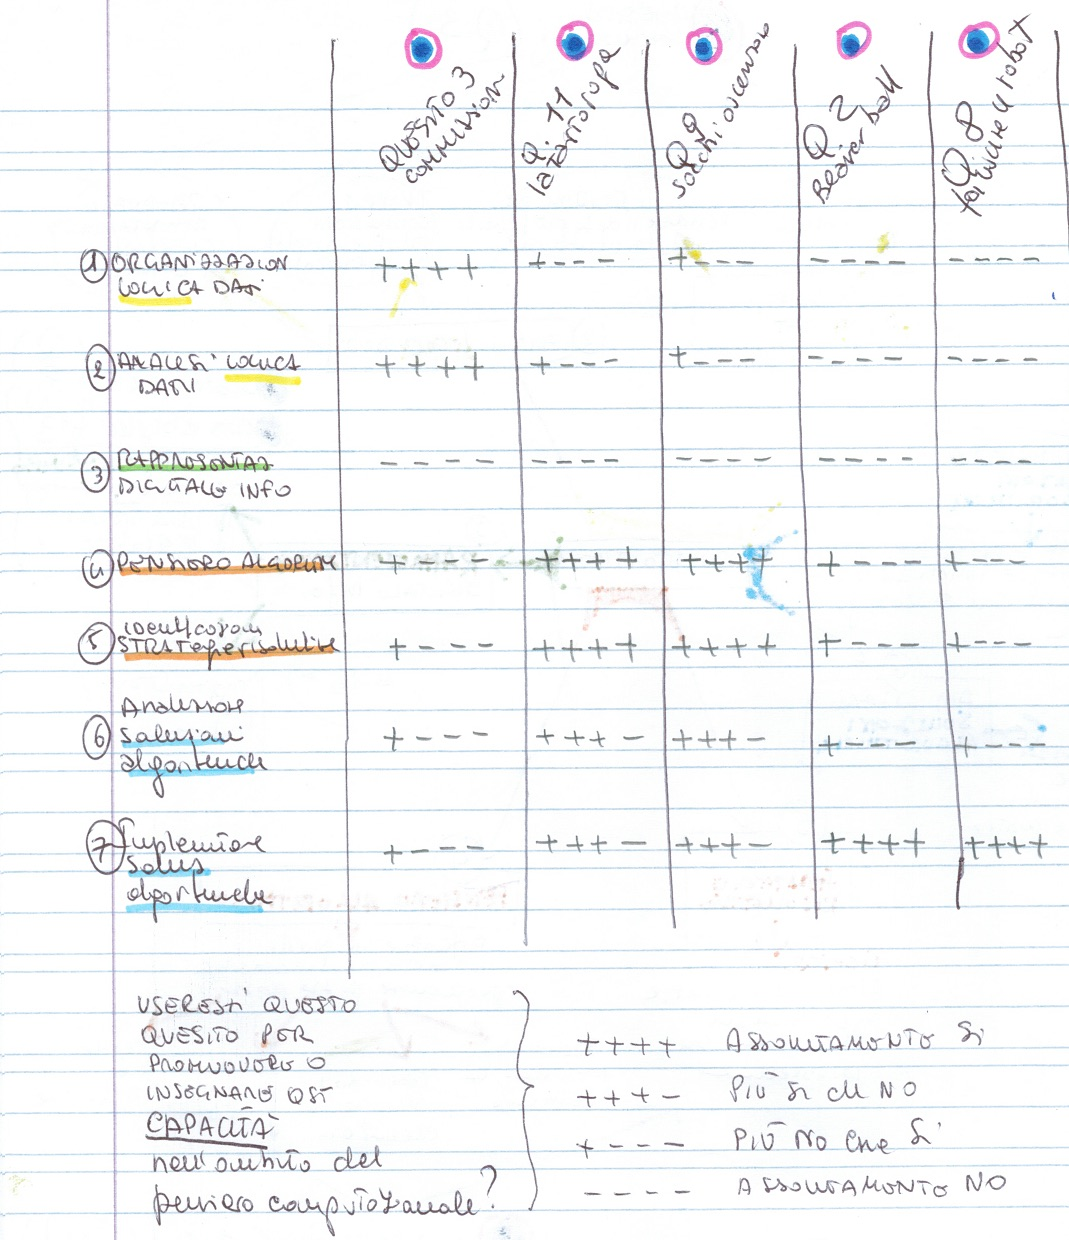
\includegraphics[width=15.0cm]{./immagini/03_Cap3/classificazione_insegnanti}}
	\caption{Esempio di risposta di una docente alla scheda proposta per l'intervista}\label{classificazione_insegnanti}
\end{figure}

\begin{figure}[htb]
	\centering
	\fbox{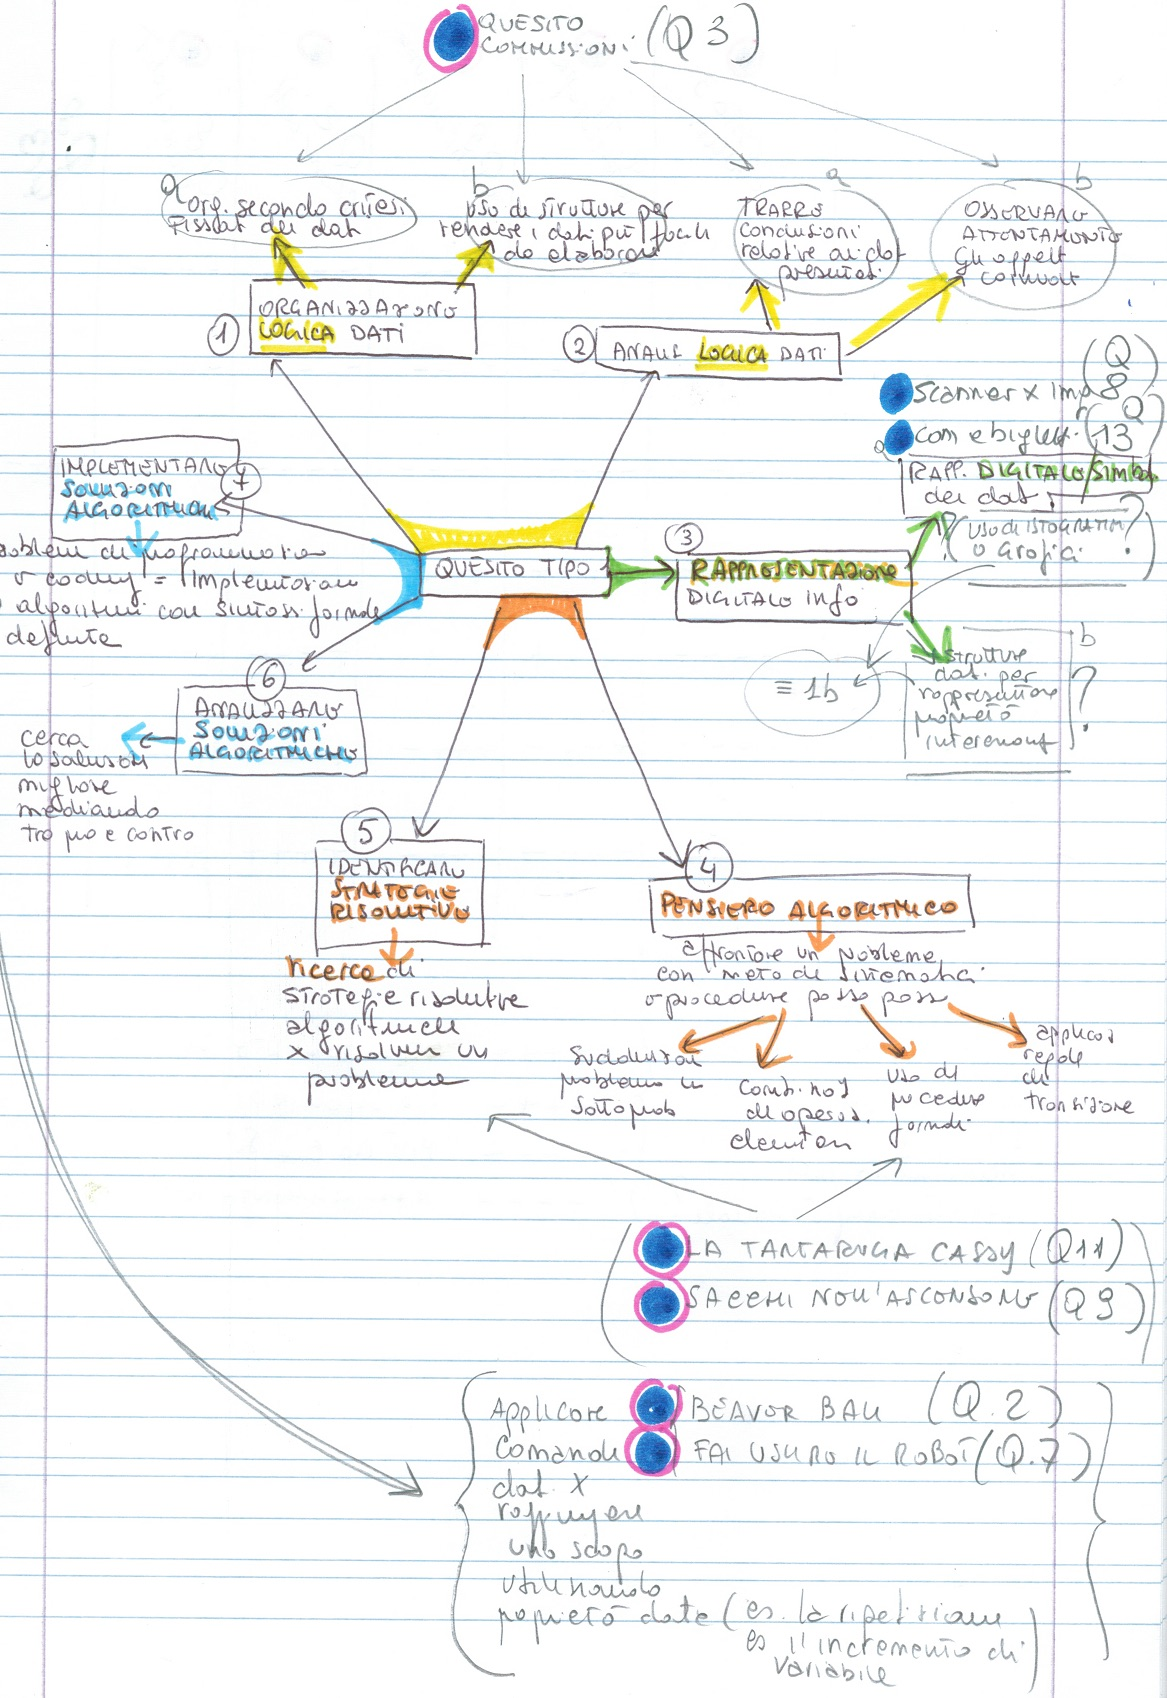
\includegraphics[width=15.0cm]{./immagini/03_Cap3/rielaborazioneCT}}
	\caption{Schema prodotto da una docente (scuola secondaria di primo grado, Matematica e Scienze) come rielaborazione della scheda proposta per l'intervista}\label{rielaborazioneCT}
\end{figure}


%Le interviste condotte sono state spunto di riflessioni e osservazioni molto interessanti che presenteremo di seguito ripercorrendo le domande guida esposte:
	
Durante le interviste abbiamo notato che, nonostante lo sforzo di rimuovere o ridurre al minimo i tecnicismi informatici, la descrizione delle abilità del pensiero computazionale contiene ancora alcuni termini i cui significati andrebbero chiariti ulteriormente. 
In particolar modo i docenti della scuola primaria hanno trovato molto difficile la comprensione dei termini \textit{problem solving} e \textit{algoritmo} che risultano essere parole con le quali questi insegnanti hanno poca familiarità. 
Anche i termini \textit{implementare} e \textit{codificare} non sono noti a tutti i docenti: in alcuni casi durante l'intervista è stato necessario aggiungere ulteriori spiegazioni a riguardo.


Un'altra osservazione che ci è stata fatta, durante le interviste, è che la ripetizione della locuzione \textit{proprietà interessanti} sia in ``Organizzazione logica dei dati'' sia in ``Rappresentazione digitale delle informazioni'' confonde nella distinzione tra le due abilità. Nella prima abilità si intende l'evidenziare di alcune caratteristiche utili all'organizzazione dei dati, mentre nel secondo caso l'intenzione principale è non perdere nessuna informazione nella rappresentazione. Potrebbe in effetti essere chiarita più esplicitamente nelle descrizioni precisando meglio cosa si intende per \textit{interessante} nei due diversi casi.


Nella richiesta di motivare alcune associazioni discordanti con le nostre, sono emerse ambiguità sul significato di alcuni termini: nella nostra accezione informatica \textit{problema} e \textit{soluzione} sono usati per riferirsi a problemi e soluzioni computazionali, mentre nella scuola elementare per \textit{problema} si intende quello che in informatica si chiamerebbe \textit{istanza di un problema}. Allo stesso modo per i docenti della scuola primaria, senza una formazione informatica, una \textit{soluzione} è semplicemente una risposta ad un problema, mentre per gli informatici questa parola è intesa come \textit{soluzione computazionale per un problema (computazionale)}, ovvero un metodo automatico per trovare la risposta corretta a qualsiasi istanza del problema. 

Altre espressioni che sono state oggetto di incomprensioni sono quelle riguardanti la rappresentazione dei dati e la loro organizzazione. In informatica la rappresentazione digitale è la traduzione delle informazioni in forma adatta alla memorizzazione e alla manipolazione da parte di un calcolatore automatico. Invece gli insegnanti hanno associato i quesiti in cui viene richiesta la codifica di un oggetto all'organizzazione logica dei dati, motivando questa scelta con l'operazione di riorganizzazione mentale degli oggetti a disposizione. Infatti per i docenti della primaria \textit{rappresentare} significa \textit{fare un quadro, dare una descrizione} e questo porta ad una incomprensione sui termini utilizzati. 




Abbiamo osservato che spesso venivano associati al pensiero algoritmico tutti i quesiti in cui è richiesto un pensiero genericamente analitico. Il processo di organizzare mentalmente la risoluzione di un problema per passi successivi uno conseguente all'altro veniva inteso come pensiero algoritmico nonostante non fossero coinvolti algoritmi o procedure da eseguire o regole formali. Ad esempio il quesito ``Braccialetti'', riportato nella Sezione 2.2 in Figura \ref{fig:braccialetti}, è stato collegato dagli insegnanti della scuola primaria al pensiero algoritmico: nel quesito vengono proposte quattro possibili soluzioni e il processo di analisi e confronto per il raggiungimento della soluzione è stato riferito all'uso di procedure passo-passo e la scomposizione del problema in sotto-problemi. Nella scuola primaria questo tipo di confusione potrebbe essere considerato accettabile, tuttavia per i ragazzi della secondaria deve essere ben distinto il pensiero analitico da quello algoritmico per poter apprezzare il vero valore del pensiero computazionale.


Per i docenti della primaria è stato piuttosto difficoltosa l'associazione dei quesiti con ``Identificare strategie risolutive'' e ``Analizzare soluzioni algoritmiche''. In effetti ai bambini si propongono di solito istanze specifiche di problemi e non classi di problemi nella loro generalità. Si chiede loro di trovare quindi la risposta a un'istanza specifica e non stabilire un metodo risolutivo generale. In altri termini, a quest'età si ragiona ad un livello di astrazione inferiore, e anche gli insegnanti, abituati a quei contesti, hanno poca familiarità con questo tipo di approccio. A conferma di questa interpretazione abbiamo verificato che i quesiti Bebras proposti nella categoria KiloBebras noi assoceremmo a queste abilità sono decisamente rari.



Nonostante queste criticità, una volta chiariti i termini e il loro uso, in generale abbiamo trovato corrispondenza per quanto riguarda la maggior parte delle associazioni tra i quesiti e le abilità. Questo conferma l'ipotesi che tali definizioni delle abilità del pensiero computazionale sono comprensibili anche a coloro che non hanno una formazione specifica in informatica. Gli insegnanti inoltre hanno apprezzato questo approccio nella discussione dei quesiti Bebras; come osservato da una docente stessa durante l'intervista: ``Questo tipo di presentazione rende i quesiti maggiormente utilizzabili nella didattica perché esprimendo le abilità sottese in maniera più esplicita si può scegliere con maggior cognizione di causa su cosa si vuole lavorare e come''.
La lettura attraverso la lente delle abilità del pensiero computazionale sembra quindi favorire l'identificazione del potenziale formativo dei quesiti Bebras e dunque rende più facile l'utilizzo in classe.


%%%%%%%%%%
% CONCLUSIONI
\chapter*{Conclusioni}
\addcontentsline{toc}{chapter}{Conclusioni}
In questa tesi è stato descritto il lavoro di analisi svolto sui quesiti Bebras mettendoli in corrispondenza con le Indicazioni Nazionali e con la classificazione basata sulla definizione operazionale di pensiero computazionale. \`{E} stato affrontato uno studio approfondito dei riferimenti ministeriali per le scuole del primo ciclo in cui si sono rilevati diversi punti relativi alla didattica dell'informatica come disciplina scientifica. Per ogni traguardo e obiettivo ministeriale con un ``sentore informatico'' si è cercato il relativo quesito Bebras che potesse essere utilizzato come strumento didattico per sviluppare l'abilità espressa. Dopo aver notato un'ottima percentuale di corrispondenze, è nata l'esigenza di rendere ancora più fruibili i quesiti Bebras come strumento didattico al di fuori delle gare annuali. Si è quindi sviluppata una classificazione basata sulla definizione operazionale di pensiero computazionale per evidenziare il potenziale valore educativo di ogni quesito.
Sono quindi state svolte delle interviste ad alcuni docenti di varie scuole per verificare se la classificazione proposta fosse comprensibile anche a coloro che non hanno una formazione informatica, ed anche utile per una eventuale progettazione all'interno del curricolo scolastico.
I docenti hanno mostrato interesse nell'uso dei quesiti all'interno della pratica scolastica, per questo motivo successivamente è stata creata un'applicazione web in cui poter ricercare i quesiti Bebras sia con la lente di lettura delle Indicazioni Nazionali che del pensiero computazionale. Inoltre per ogni quesito si può facilmente reperire la relativa soluzione e spiegazione.

\`{E} stato ipotizzato un possibile ampliamento dell'applicazione web: la possibilità per i docenti di commentare i quesiti Bebras riportando le proprie esperienze didattiche 
o anche annotare delle osservazioni che permettano agli organizzatori della gara Bebras di avere dei feedbacks puntuali sui quesiti specifici.


%%%%%%%%%%%%%%
\appendix

\chapter{Indicazioni nazionali affini all'informatica} \label{ElencoIndicazioni}
Di seguito vengono riportati i traguardi e gli obiettivi delle indicazioni nazionali \cite{indicazioniNazionali} che sono risultati attinenti all'insegnamento dell'informatica.

\bigskip
\noindent \textbf{MATEMATICA}
\\
Gradualmente, stimolato dalla guida dell'insegnante e dalla discussione con i pari, l’alunno imparerà ad affrontare con fiducia e determinazione situazioni problematiche, rappresentandole in diversi modi, conducendo le esplorazioni opportune, dedicando il tempo necessario alla precisa individuazione di ciò che è noto e di ciò che s'intende trovare, congetturando soluzioni e risultati, individuando possibili strategie risolutive. Nella scuola secondaria di primo grado si svilupperà un'attività più propriamente di matematizzazione, formalizzazione, generalizzazione.
L'alunno analizza le situazioni per tradurle in termini matematici, riconosce schemi ricorrenti, stabilisce analogie con modelli noti, sceglie le azioni da compiere (operazioni, costruzioni geometriche, grafici, formalizzazioni, scrittura e risoluzione di equazioni, ...) e le concatena in modo efficace al fine di produrre una risoluzione del problema. Un’attenzione particolare andrà dedicata allo sviluppo della capacità di esporre e di discutere con i compagni le soluzioni e i procedimenti seguiti.


\bigskip
\textbf{Traguardi per lo sviluppo delle competenze al termine della scuola primaria}
\begin{itemize}
	\item Descrive, denomina e classifica figure in base a caratteristiche geometriche, ne determina misure, progetta e costruisce modelli concreti di vario tipo.
	\item Ricerca dati per ricavare informazioni e costruisce rappresentazioni (tabelle e grafici). Ricava informazioni anche da dati rappresentati in tabelle e grafici.
	\item Legge e comprende testi che coinvolgono aspetti logici e matematici.
	\item Riesce a risolvere facili problemi in tutti gli ambiti di contenuto, mantenendo il controllo sia sul processo risolutivo, sia sui risultati. Descrive il procedimento seguito e riconosce strategie di soluzione diverse dalla propria.
	\item Costruisce ragionamenti formulando ipotesi, sostenendo le proprie idee e confrontandosi con il punto di vista di altri.
	\item Sviluppa un atteggiamento positivo rispetto alla matematica, attraverso esperienze significative, che gli hanno fatto intuire come gli strumenti matematici che ha imparato ad utilizzare siano utili per operare nella realtà.
\end{itemize}

\medskip
\noindent \textbf{Obiettivi di apprendimento al termine della classe terza della scuola primaria}
\begin{description}
	\item \textit{Spazio e figure}
		\begin{itemize}
			\item Comunicare la posizione di oggetti nello spazio fisico, sia rispetto al soggetto, sia rispetto ad altre persone o oggetti, usando termini adeguati (sopra/sotto, davanti/dietro, destra/sinistra, dentro/fuori).
			\item Eseguire un semplice percorso partendo dalla descrizione verbale o dal disegno, descrivere un percorso che si sta facendo e dare le istruzioni a qualcuno perché compia un percorso desiderato.
			\item Riconoscere, denominare e descrivere figure geometriche.
		\end{itemize}
\medskip
	\item \textit{Relazioni, dati e previsioni}
		\begin{itemize}
			\item Classificare numeri, figure, oggetti in base a una o più proprietà, utilizzando rappresentazioni opportune, a seconda dei contesti e dei fini.
			\item Argomentare sui criteri che sono stati usati per realizzare classificazioni e ordinamenti assegnati.
			\item Leggere e rappresentare relazioni e dati con diagrammi, schemi e tabelle.
		\end{itemize}
\end{description}

\medskip
\noindent \textbf{Obiettivi di apprendimento al termine della classe quinta della scuola primaria}
\begin{description}
	\item \textit{Spazio e figure}
	\begin{itemize}
		\item Descrivere, denominare e classificare figure geometriche, identificando elementi significativi e simmetrie, anche al fine di farle riprodurre da altri.
		\item Riconoscere figure ruotate, traslate e riflesse.
	\end{itemize}
	\medskip
	\item \textit{Relazioni, dati e previsioni}
	\begin{itemize}
		\item Rappresentare relazioni e dati e, in situazioni significative, utilizzare le rappresentazioni per ricavare informazioni, formulare giudizi e prendere decisioni.
		\item Rappresentare problemi con tabelle e grafici che ne esprimono la struttura.
		\item In situazioni concrete, di una coppia di eventi intuire e cominciare ad argomentare qual è il più probabile, dando una prima quantificazione nei casi più semplici, oppure riconoscere se si tratta di eventi ugualmente probabili.
		\item Riconoscere e descrivere regolarità in una sequenza di numeri o di figure.
	\end{itemize}
\end{description}

\bigskip
\noindent \textbf{Traguardi per lo sviluppo delle competenze al termine della scuola secondaria di primo grado}
\begin{itemize}
	\item Analizza e interpreta rappresentazioni di dati per ricavarne misure di variabilità e prendere decisioni.
	\item Riconosce e risolve problemi in contesti diversi valutando le informazioni e la loro coerenza.
	\item Spiega il procedimento seguito, anche in forma scritta, mantenendo il controllo sia sul processo risolutivo, sia sui risultati.
	\item Confronta procedimenti diversi e produce formalizzazioni che gli consentono di passare da un problema specifico a una classe di problemi.
	\item Produce argomentazioni in base alle conoscenze teoriche acquisite (ad esempio sa utilizzare i concetti di proprietà caratterizzante e di definizione).
	\item Sostiene le proprie convinzioni, portando esempi e controesempi adeguati e utilizzando concatenazioni di affermazioni; accetta di cambiare opinione riconoscendo le conseguenze logiche di una argomentazione corretta.
	\item Utilizza e interpreta il linguaggio matematico (piano cartesiano, formule, equazioni, ...) e ne coglie il rapporto col linguaggio naturale.
\end{itemize}

\medskip
\noindent \textbf{Obiettivi di apprendimento al termine della classe terza della scuola secondaria di primo grado}
\begin{description}
	\item \textit{Numeri}
	\begin{itemize}
		\item Eseguire addizioni, sottrazioni, moltiplicazioni, divisioni, ordinamenti e confronti tra i numeri conosciuti (numeri naturali, numeri interi, frazioni e numeri decimali), quando possibile a mente oppure utilizzando gli usuali algoritmi scritti, le calcolatrici e i fogli di calcolo e valutando quale strumento può essere più opportuno.
	\end{itemize}
	\medskip
	\item \textit{Dati e previsioni}
	\begin{itemize}
		\item Rappresentare insiemi di dati, anche facendo uso di un foglio elettro- nico. In situazioni significative, confrontare dati al fine di prendere decisioni, utilizzando le distribuzioni delle frequenze e delle frequenze relative. Scegliere ed utilizzare valori medi (moda, mediana, me- dia aritmetica) adeguati alla tipologia ed alle caratteristiche dei dati a disposizione. Saper valutare la variabilità di un insieme di dati determinandone, ad esempio, il campo di variazione.
		\item Riconoscere coppie di eventi complementari, incompatibili, indipendenti.
	\end{itemize}
\end{description}

\bigskip
\noindent \textbf{SCIENZE}
\\
\textbf{Traguardi per lo sviluppo delle competenze al termine della scuola primaria}
\begin{itemize}
	\item Individua nei fenomeni somiglianze e differenze, fa misurazioni, registra dati significativi, identifica relazioni spazio/temporali.
	\item Individua aspetti quantitativi e qualitativi nei fenomeni, produce rappresentazioni grafiche e schemi di li vello adeguato, elabora semplici modelli.
\end{itemize}

\medskip
\noindent \textbf{Obiettivi di apprendimento al termine della classe terza di scuola primaria}
\begin{description}
	\item \textit{Esplorare e descrivere oggetti e materiali}
	\begin{itemize}
		\item Seriare e classificare oggetti in base alle loro proprietà.
	\end{itemize}
\end{description}

\bigskip
\noindent \textbf{TECNOLOGIA}
\\
Quando possibile, gli alunni potranno essere introdotti ad alcuni linguaggi di programmazione particolarmente semplici e versatili che si prestano a sviluppare il gusto per l'ideazione e la realizzazione di progetti (siti web interattivi, esercizi, giochi, programmi di utilità) e per la comprensione del rapporto che c'è tra codice sorgente e risultato visibile.


\medskip
\noindent \textbf{Obiettivi di apprendimento al termine della classe quinta della scuola primaria}
\begin{description}
	\item \textit{Vedere e osservare}
	\begin{itemize}
		\item Rappresentare i dati dell'osservazione attraverso tabelle, mappe, diagrammi, disegni, testi.
	\end{itemize}
\end{description}


\bigskip 
\noindent \textbf{Traguardi per lo sviluppo delle competenze al termine della scuola secondaria di primo grado}
\begin{itemize}
	\item Sa utilizzare comunicazioni procedurali e istruzioni tecniche per eseguire, in maniera metodica e razionale, compiti operativi complessi, anche collaborando e cooperando con i compagni.
	\item Progetta e realizza rappresentazioni grafiche o iconografiche, relative alla struttura e al funzionamento di sistemi materiali o immateriali, utilizzando elementi del disegno tecnico o altri linguaggi multimediali e di programmazione.
\end{itemize}

\medskip
\noindent \textbf{Obiettivi di apprendimento al termine della classe terza della scuola secondaria di primo grado}
\begin{description}
	\item \textit{Prevedere, immaginare e progettare}
	\begin{itemize}
		\item Valutare le conseguenze di scelte e decisioni relative a situazioni problematiche.
	\end{itemize}
	\item \textit{Intervenire, trasformare e produrre}
	\begin{itemize}
		\item Utilizzare semplici procedure per eseguire prove sperimentali nei vari settori della tecnologia (ad esempio: preparazione e cottura degli alimenti).
		\item Programmare ambienti informatici e elaborare semplici istruzioni per controllare il comportamento di un robot.
	\end{itemize}
\end{description}
%%%%%%%%%%%%%%

\chapter{Applicazione web per i quesiti Bebras} \label{Applicazione} 
% per la consultazione dei quesiti Bebras
I quesiti Bebras, come visto nel Capitolo 3, possono essere un interessante strumento per l'insegnamento curricolare dell'informatica e per l'acquisizione del pensiero computazionale. Per rendere questa risorsa disponibile a tutti i docenti interessati, abbiamo creato una piattaforma web che raccoglie tutti i quesiti disponibili.
Attualmente i quesiti delle edizioni italiane sono già a disposizione, sotto forma di esercitazione, sulla piattaforma di gara \cite{PiattaformaBebras} ma essa risulta difficile da consultare per la ricerca di un singolo quesito o di uno specifico argomento.
Abbiamo quindi ritenuto opportuno offrire la possibilità di ricercare un dato quesito sia attraverso la lente di lettura delle Indicazioni Nazionali presentate nel Capitolo 2, sia tramite le abilità del pensiero computazionale esposte nel Capitolo 3.
\section{Tecnologie utilizzate}

\subsection{MongoDB}
MongoDB \cite{mongoDB}è un DBMS open-source orientato ai documenti. Rientra nella categoria dei DBMS NoSQL infatti, anzichè utilizzare una struttura basata su tabelle come i database relazionali, MongoDB memorizza i dati in documenti JSON-like con schema dinamico (formato che prende il nome di BSON). Questa strategia mira ad avere migliori prestazioni rispetto ai RDBMS tradizionali, una disponibilità dei dati più elevata e una scalabilità orizzontale su cluster che viene automatizzata grazie a un sistema chiamato sharding. I dati vengono organizzati in record chiamati documenti, ovvero strutture dati composte da coppie campo-valore. I valori associati ai campi possono contenere a loro volta altri documenti, array o array di documenti.
Questo annidamento di documenti e array consente di diminuire il numero di oggetti archiviati e di ovviare all'impossibilità di effettuare operazioni di join su documenti memorizzati in modo distribuito. Anziché usare tabelle, infatti, i documenti vengono organizzati in collezioni, tra le quali non è possibile effettuare operazioni di join in modo diretto. La robustezza del sistema viene incrementata da un sistema di ridondanza automatizzato. MongoDB presenta comunque degli svantaggi, infatti il suo sistema di indicizzazione dei dati determina un uso massiccio della memoria, e in quanto a spazio su disco, mediamente comporta un'occupazione maggiore rispetto ai DBMS relazionali.

In particolare per lo sviluppo di questa applicazione web viene utilizzata la piattaforma mLab \cite{mLab}: un servizio di database cloud che ospita database MongoDB.


\subsection{Flask}
Flask è un framework web scritto in Python e basato sullo strumento WSGI e con il motore template Jinja2.

WSGI (Web Server Gateway Interface) è un protocollo di trasmissione che stabilisce e descrive comunicazioni ed interazioni tra server ed applicazioni web scritte nel linguaggio Python. \`{E} quindi l'interfaccia standard del web service per la programmazione in Python.
In altre parole, il protocollo specifica come i server si facciano carico delle richieste provenienti dai browser/client ed inoltrino le informazioni richieste alle relative applicazioni, oltre a come utilizzare le informazioni di cui si sono fatti carico e a come rispondere.

Jinja2 è un motore di template per il linguaggio Python.


L’aggettivo che descrive meglio Flask, a detta degli stessi sviluppatori, è “micro”, con il quale non si intende tracciare i limiti del framework bensì il suo essere essenziale. Nonostante sia decisamente snello, offre una vasta serie di estensioni che consentono di personalizzarne le funzionalità secondo le proprie esigenze.

\section{Descrizione delle funzionalità}
In questa sezione saranno presentate le funzionalità dell'applicazione sviluppata attraverso i casi d'uso più significativi.


Nella homepage (Figura \ref{App_homepage}) l'utente può scegliere se visionare l'intero elenco dei quesiti Bebras disponibili oppure cercare uno o più quesiti in relazione alle Indicazioni Nazionali o in base alle abilità del pensiero computazionale.


Nella sezione ``Elenco quesiti'' vengono visualizzati tutti i quesiti italiani Bebras in un elenco (Figura  \ref{App_elencoQuesiti}) su cui si possono applicare i filtri di ricerca per \textit{Anno} e/o \textit{Categoria}, oppure cercare un dato quesito attraverso il suo titolo.
Selezionando il quesito d'interesse si ottiene il suo dettaglio (Figura \ref{App_dettaglioQuesito}):

\begin{itemize}
	\item Testo quesito 
	\item Soluzione e spiegazione
	\item Argomento informatico: si indica la tematica informatica trattata nel quesito in questione
	\item Traguardi e obiettivi ministeriali: vengono indicati i traguardi e gli obiettivi delle Indicazioni Nazionali collegati al quesito in questione
	\item Esporta in PDF: è possibile scegliere quali dei dettagli elencati precedentemente inserire nel documento pdf che si vuole creare
\end{itemize}

Nella sezione ``Indicazioni nazionali'' (Figura \ref{indicazioniNazionali}) vengono proposti i traguardi e gli obiettivi affini all'informatica (Appendice \ref{ElencoIndicazioni}) estratti dal documento del Ministero \cite{indicazioniNazionali}. In questa sezione il docente può scegliere la materia, il grado scolastico e il traguardo o obiettivo di interesse ed ottenere i relativi quesiti Bebras.

Nella sezione ``Pensiero computazionale'' (Figura \ref{App_CT}) sono riportate le descrizioni delle abilità del pensiero computazionale che sono state esposte nella Sezione \ref{interviste}. Per ogni abilità presentata il docente può reperire l'elenco dei quesiti Bebras che la promuovono.

\begin{figure}[H]
	\centering
	\fbox{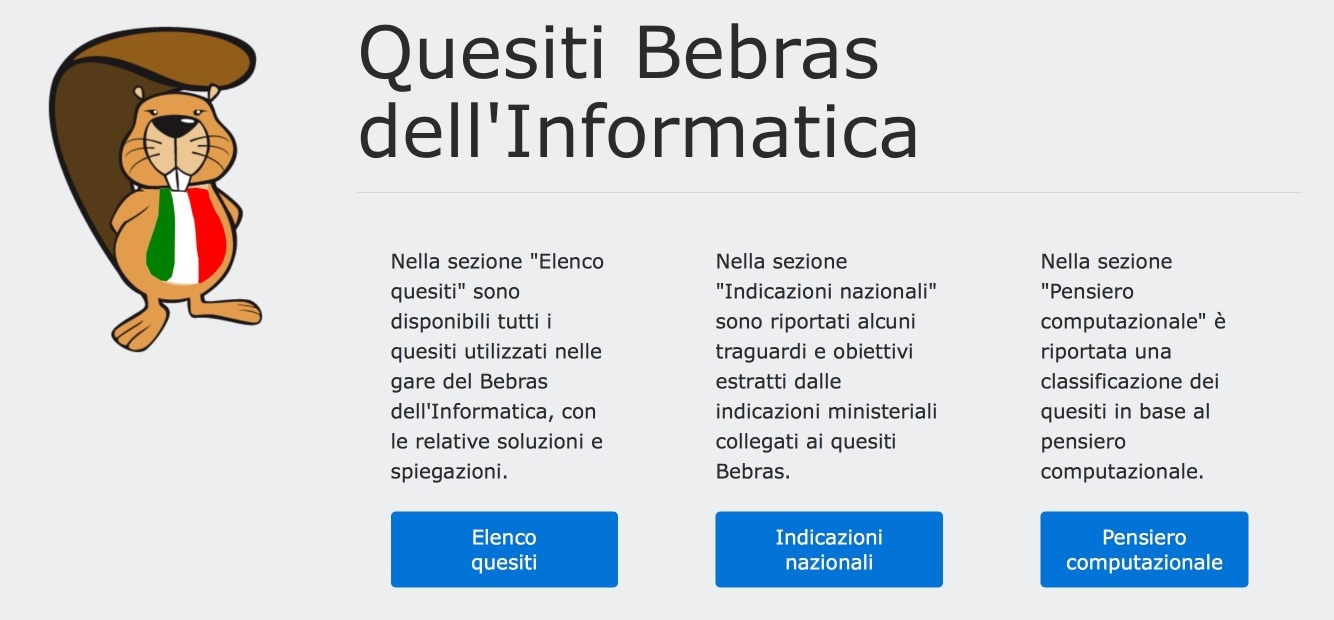
\includegraphics[width=14.8cm]{./immagini/Appendice/App_homepage}}
	\caption{Homepage dell'applicazione web}
	\label{App_homepage}
\end{figure}

\begin{figure}[H]
	\centering
	\fbox{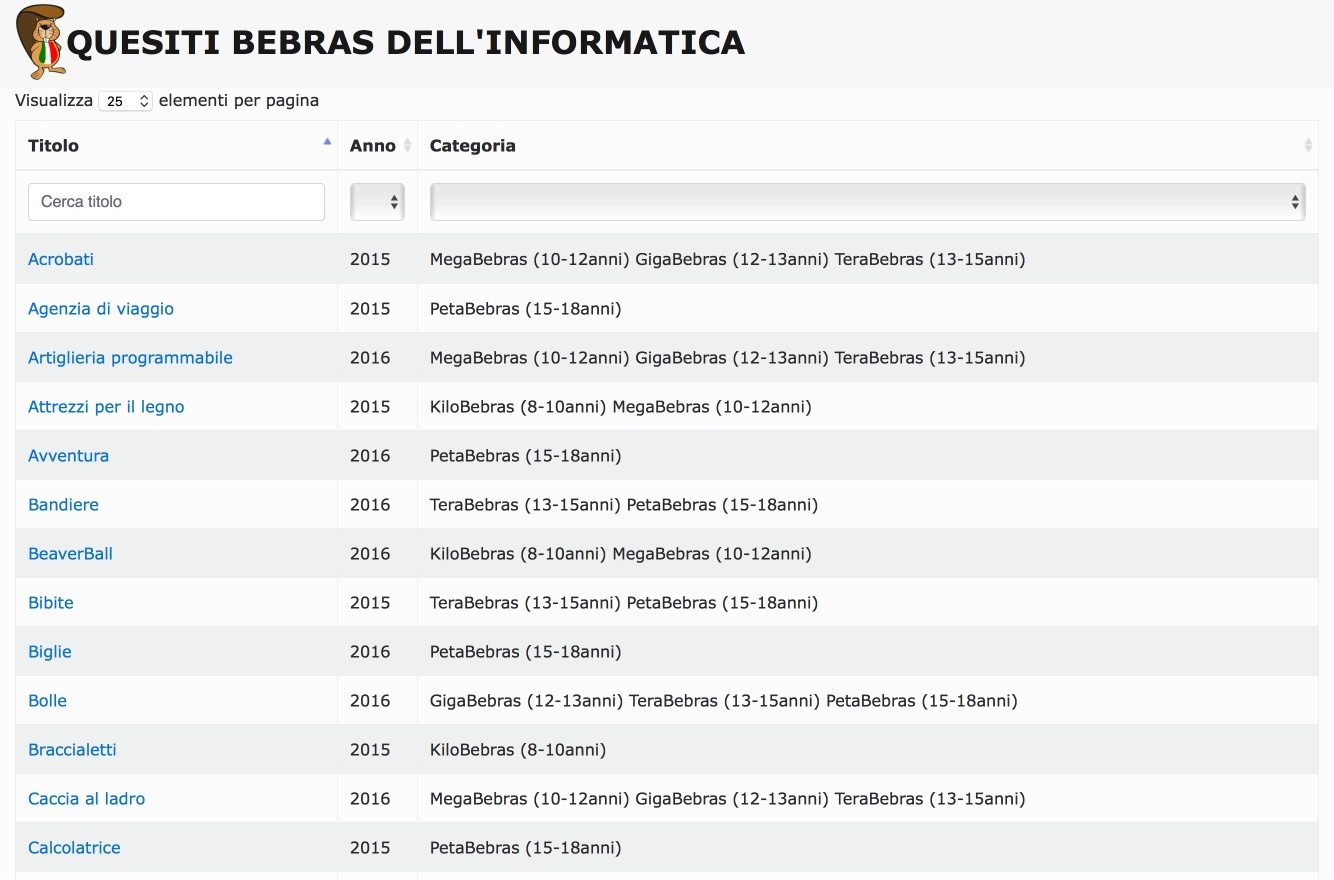
\includegraphics[width=14.8cm]{./immagini/Appendice/App_elencoQuesiti}}
	\caption{Elenco quesiti Bebras}
	\label{App_elencoQuesiti}
\end{figure}

\begin{figure}[H]
	\centering
	\fbox{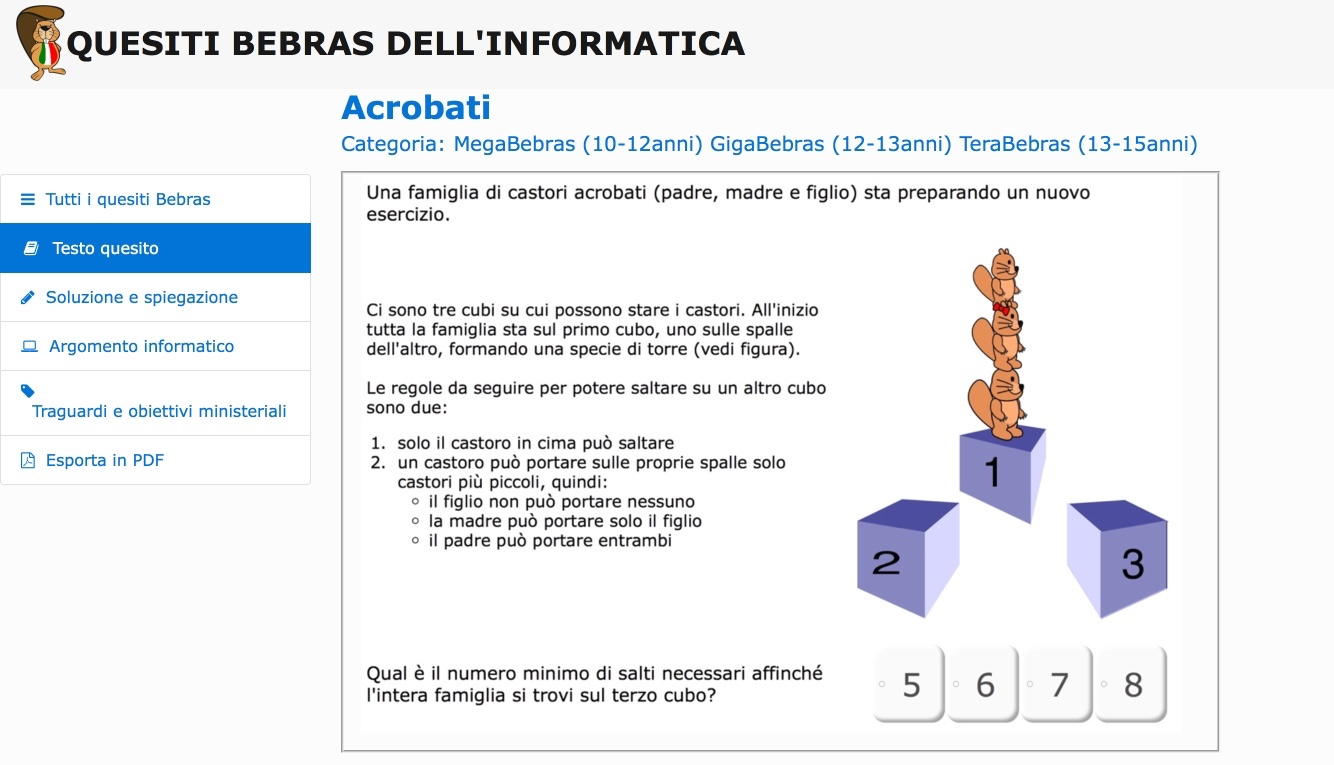
\includegraphics[width=14cm]{./immagini/Appendice/App_dettaglioQuesito}}
	\caption{Dettaglio di un quesito Bebras}
	\label{App_dettaglioQuesito}
\end{figure}


\begin{figure}[H]
	\centering
	\fbox{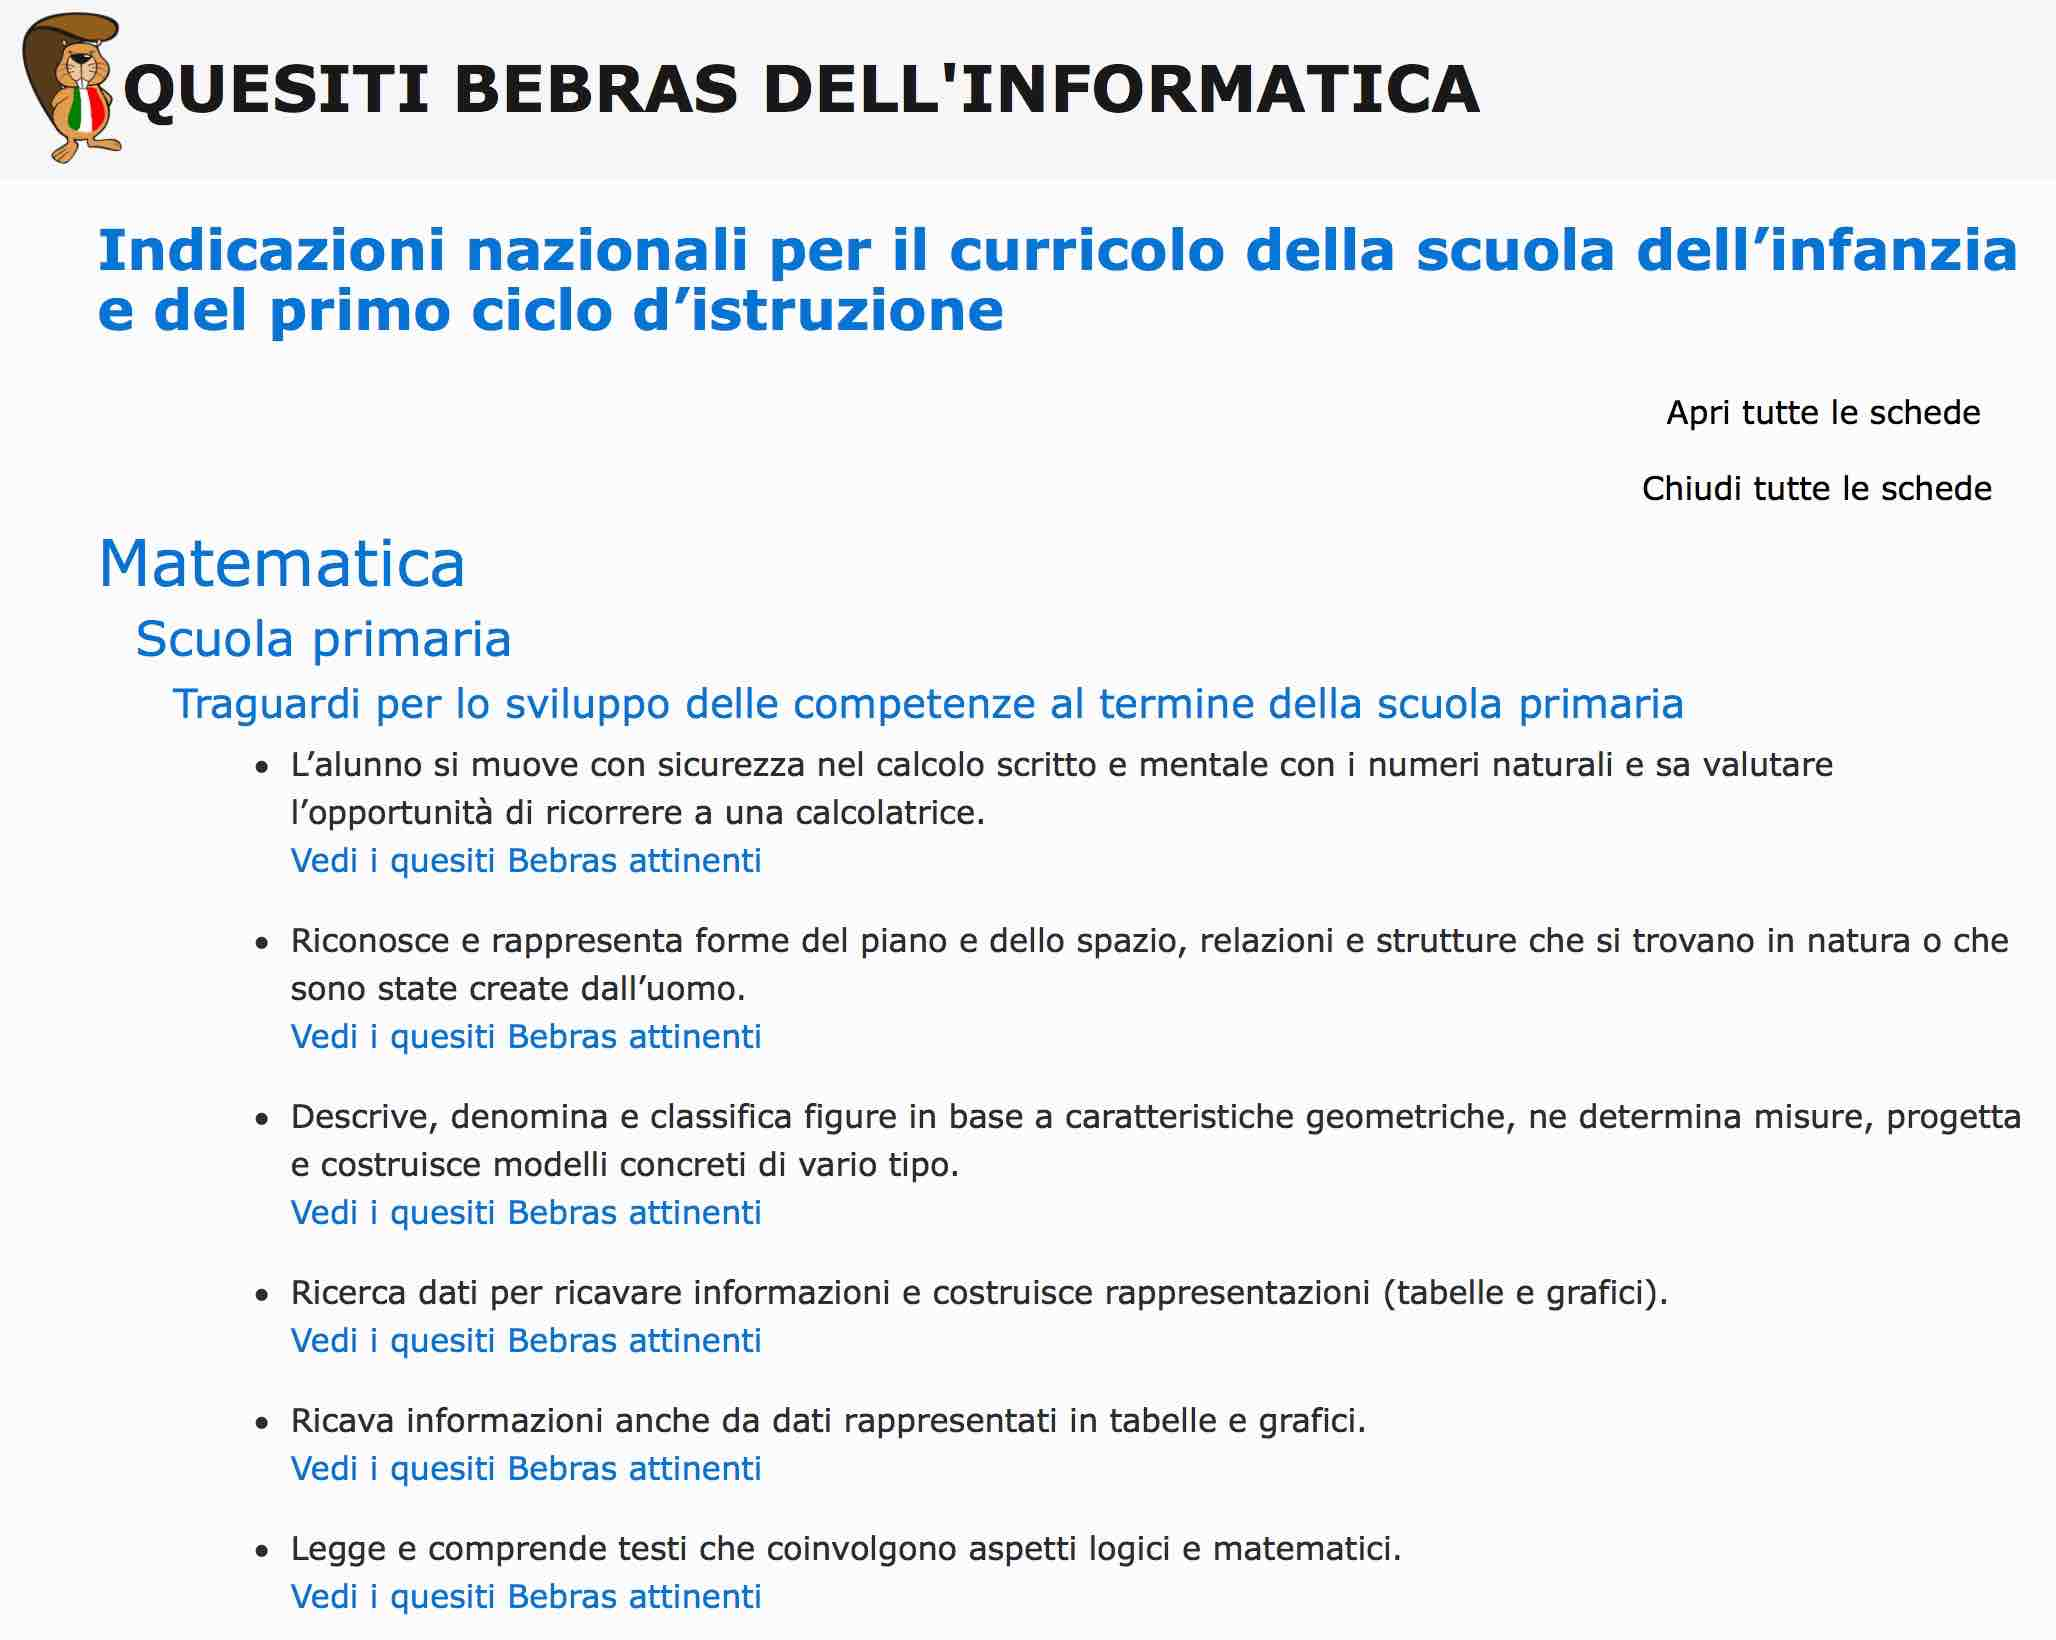
\includegraphics[width=12cm]{./immagini/Appendice/02_SitoIndicazioni}} \label{indicazioniNazionali}
	\caption{Elenco delle Indicazioni Nazionali affini all'informatica}
\end{figure}


\begin{figure}[H]
	\centering
	\fbox{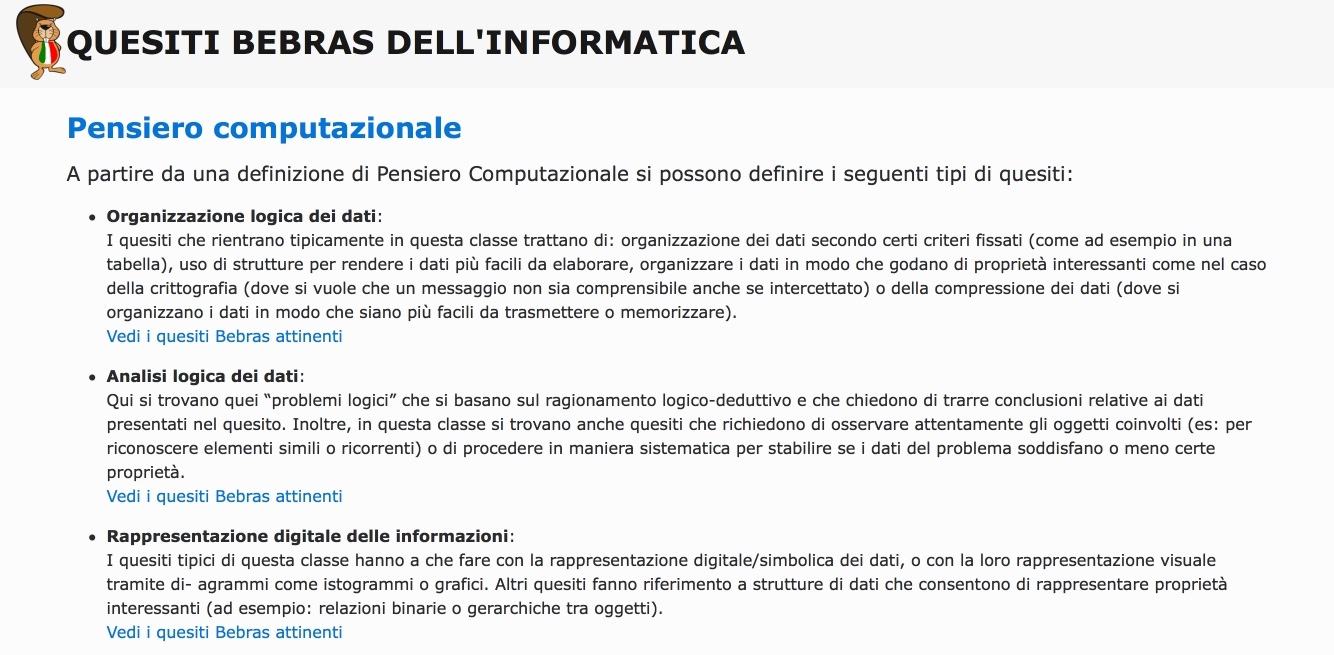
\includegraphics[width=15.0cm]{./immagini/Appendice/App_CT}}
	\caption{Elenco delle abilità del pensiero computazionale}
	\label{App_CT}
\end{figure}

%%%%%%%%%%
%			BIBLIOGRAFIA
%
\begin{thebibliography}{00}
%
\bibitem{BellettiniITICSE2015}
C. Bellettini, V. Lonati, D. Malchiodi, M. Monga, A. Morpurgo, M. Torelli, 
``How challenging are Bebras tasks? An IRT analysis based on the performance of Italian students'', 
Proceedings of the 2015 ACM Conference on Innovation and Technology in Computer Science Education (ITiCSE 2015), 
pp. 27-32, 
Lithuania, 
July, 6-8, 
2015.
%
\bibitem{DagieneIFIP2010}
V. Dagiene, G. Futschek, 
``Introducing Informatics Concepts through a Contest'', 
IFIP working conference: New developments in ICT and education, 
Amiens: Universite de Picardie Jules Verne, 
2010.
%
\bibitem{LonatiITICSE2017}
V. Lonati, D. Malchiodi, M. Monga, A. Morpurgo, 
``Bebras as a teaching resource: classifying the tasks corpus using computational thinking skills'', 
Proceedings of the 22nd annual conference on innovation and technology in computer science education (ITiCSE 2017) 
Bologna, Italy, 
2017.
%
\bibitem{DagieneISEEP2008}
V. Dagiene, G. Futschek, 
``Bebras international contest on informatics and computer literacy: Criteria for good tasks'', 
ISSEP 2008, 
LNCS, vol. 5090, 
pp. 19–30, 
2008.
%
\bibitem{PohlQuality}
W. Pohl, H.W. Hein,
``Aspects of quality in the presentation of informatics challenge tasks'', 
LNCS, vol. 9378, 
pp. 21–32,
2015.
%
\bibitem{WilemDifficulty}
W. Van der Vegt, 
``Predicting the difficulty level of a Bebras task'',
Olympiads in Informatics,
vol. 7, 
pp. 132-139,
2013.
%
\bibitem{DagieneINFORMATICA2017}
V. Dagiene, S. Sentence, G. Stupuriene, 
``Developing a Two-Dimensional Categorization System for Educational Tasks in Informatics'', 
Informatica, vol. 28, no.1, 
pp.23-44, 
2017.
%
\bibitem{flayerCT}
International Society for Technology in Education \& Computer Science Teachers Association, 
``Operational definition of computational thinking for K-12 education.''
\url{https://csta.acm.org/Curriculum/sub/ CurrFiles/CompThinkingFlyer.pdf}, 
2011.
%
\bibitem{DagieneISSEP2016}
V. Dagiene, S. Sentance, 
``It’s computational thinking! bebras tasks in the curriculum'', 
ISSEP 2016, 
LNCS, vol. 9973, 
pp. 28–39, 
2016.
%
\bibitem{indicazioniNazionali}
Indicazioni nazionali riguardanti gli obiettivi specifici di apprendimento concernenti le attività e gli insegnamenti compresi nei piani degli studi previsti per i percorsi liceali di cui all'art. 10, comma 3, del DPR 15/3/2010, n. 89, in relazione all'art. 2, commi 1 e 3, del medesimo regolamento, 2010.
%
\bibitem{DagieneKEYCIT2015}
V. Dagiene, G. Stupuriene, 
``Informatics education based on solving attractive tasks through a contest'', 
KEYCIT 2014 - Key Competencies in Informatics and ICT, 
pp. 97 – 115, 
2015.
%
\bibitem{HabermanACM2011}
B. Haberman, A. Cohen, V. Dagiene, 
``The beaver contest: attracting youngsters to study computing'', 
Proceedings of the 16th annual joint conference on Innovation and technology in computer science education, ACM, 
p. 378, 
2011.
%
\bibitem{LonatiISSEP2017}
A. Calcagni, V. Lonati, D. Malchiodi, M. Monga, A. Morpurgo, 
``Promoting computational thinking skills: would you use this Bebras task?'', 
Proceedings of the international conference on informatics in schools: situation, evolution and perspectives (ISSEP2017) (in stampa) 
Helsinki, Finland, 
2017.
%
\bibitem{KalasIFIP2009}
I. Kalaš, M. Tomcsányiová, 
``Students’ Attitude to Programming in Modern Informatics'', 
IFIP World Conference on Computers in Education, 
Bento Goncalves, Brazil, 
2009.
%
\bibitem{PohlLNCS2015}
W. Pohl, J. Westmeyer, 
``Content categories for informatics tasks'', 
LNCS, vol.9378, 
pp. 61-62,
2015. 
%
\bibitem{SchwillEATCS1994}
A. Schwill, 
``Fundamental ideas of computer science'', 
EATCS-Bulletin, vol. 53, 
pp. 274– 295, 
1994.
%
\bibitem{Bloom}
B. S. Bloom,  
``Taxonomy of Educational Objectives. Handbook I: The Cognitive Domain.'', 
New York: David McKay Co Inc.,
1956.
%
\bibitem{Anderson}
L. W. Anderson, D. R. Krathwohl, P.W. Airasian, K.A. Cruikshank, ... M.C. Wittrock,
``A Taxonomy for Learning, Teaching, and Assessing: A revision of Bloom’s Taxonomy of Educational Objectives.'', 
New York: Pearson, Allyn \& Bacon,
2000.
%
\bibitem{LonatiKoli2017}
V. Lonati, D. Malchiodi, M. Monga, A. Morpurgo, 
``How presentation affects the difficulty of computational thinking tasks: an IRT analysis'', 
Proceedings of the 17th koli calling international conference on computing education research (in stampa),
Koli, Finland, 
2017.
%
\bibitem{BellettiniISSEP2014}
C. Bellettini, V. Lonati, D. Malchiodi, M. Monga, A. Morpurgo, M. Torelli, L. Zecca,
``Extracurricular activities for improving the perception of Informatics in Secondary schools'',
Proceedings of ISSEP 2014 - 7th International conference on informatics in Schools: Situation, Evolution, and Perspective, 
Lecture Notes in Computer Science, 
vol. 8730, pp. 161-172,
Istanbul,
22-25 September 
2014.
%
\bibitem{BellettiniTOCE2014}
C. Bellettini, V. Lonati, D. Malchiodi, M. Monga, A. Morpurgo, M. Torelli, L. Zecca,
``Informatics Education in Italian Secondary Schools'',
ACM Transactions on Computing Education (TOCE), 
vol. 14, issue 2,
June 
2014.
%
\bibitem{Mirolo2003}
Claudio Mirolo, ``Quale informatica nella scuola?'', \url{http://nid.dimi.uniud.it/pages/materials/discussion/ educazione.pdf} ,2003. 
%
\bibitem{RoyalSociety2012}
The Royal Society, ``Shut down or restart? The way forward for computing in UK schools'', \url{http: //royalsociety.org/education/policy/computing-in-schools/report/}, 2012.
%
\bibitem{InformaticaScuola}
Programma il futuro, ``Perché l'informatica nelle scuole'',
\url{https://www.programmailfuturo.it/progetto/perche-partecipare/informatica-e-scuola}
%
\bibitem{IndicazioniLicei}
Indicazioni nazionali riguardanti gli obiettivi specifici di apprendimento concernenti le attività e gli insegnamenti compresi nei piani degli studi previsti per i percorsi liceali di cui all'art. 10, comma 3, del DPR 15/3/2010, n. 89, in relazione all'art. 2, commi 1 e 3, del medesimo regolamento, \url{http://nuovilicei.indire.it/content/index.php?action=lettura_paginata&id_m=7782&id_cnt=10497}, 2010.
%
\bibitem{IndicazioniIstituti}
Istituti professionali, linee guida per il passaggio al nuovo ordinamento, \url{http://www.indire.it/lucabas/lkmw_file/nuovi_tecnici///INDIC/_LINEE_ GUIDA_TECNICI_.pdf}, \url{http://www.indire.it/lucabas/lkmw_file/nuovi_professionali///linee_guid a/_LINEE GUIDA ISTITUTI PROFESSIONALI_.pdf}, 2010.
%
\bibitem{BellettiniTFA2015}
C. Bellettini, V. Lonati, D. Malchiodi, M. Monga, A. Morpurgo, F. Pedersini, ``La formazione degli insegnanti della classe 42/A --- Informatica: l'esperienza dell'Università degli Studi di Milano'', 
E questo tutti chiamano informatica, L'esperienza dei TFA nelle discipline informatiche, 
Collana Manuali 14 Sapienza Università Editrice Roma, Italia,
2015.
%
\bibitem{BebrasInternazionale}
Bebras International Challenge on Informatics and Computational Thinking, \url{http://bebras.org} .
%
\bibitem{PiattaformaBebras}
Piattaforma delle gare Bebras in Italia, \url{https://bebras.it/students}
%
\bibitem{WingCT2006}
J. M. Wing, ``Computational Thinking”, Communications of the ACM, 
Vol. 49, No. 3, pp. 33–35,
March 
2006.
%
\bibitem{mLab}
Piattaforma mLab, \url{https://mlab.com}
%
\bibitem{mongoDB}
MongoDB, \url{https://www.mongodb.com}
%
\bibitem{INVALSI}
Invalsi, guida alla lettura prova di matematica Scuola Secondaria di primo grado \url{http://www.invalsi.it/areaprove/documenti/strumenti/PN/2014_PN_GUIDA_MATEMATICA.pdf}
%
\bibitem{PapertCT}
S. Papert, ``An exploration in the space of mathematics educations'',
International Journal of Computers for Mathematical Learning, 
pp. 95–123, 
1996.
%
\bibitem{NardelliCT}
E. Nardelli, ``Informatica nella scuola: disciplina fondamentale e trasversale, ovvero di cosa parliamo quando parliamo di pensiero computazionale'',
Scienze e ricerche Magazine,
Aprile 2017.
%
\bibitem{attitudiniCT}
V. Barr, C. Stephenson, ``Bringing computational thinking to K-12: what is Involved and what is the role of the computer science education community?'', 
ACM Inroads, 
pp. 48–54,
2011.
%
\end{thebibliography}


%%%%%%%%%%%%%%%%
% 
%			RINGRAZIAMENTI
%

%\prefacesection{Ringraziamenti}

\end{document}


 
